\documentclass[12pt, a4paper]{book}
\begin{document}\label{chap:Best_ML_MI}
\chapter{Model independent approach}
\graphicspath{{../../Plots/}}
\section{Dark Higgs Heavy Dark Sector}
\clearpage

\begin{table}[!ht]\centering\caption[Inputs for the $Z'h_D\rightarrow l^+l^-\chi\overline{\chi}$ HDS $\sigma B$ calculations in SR1]{Inputs for the $Z'h_D\rightarrow l^+l^-\chi\overline{\chi}$ HDS $\sigma B$ calculations in SR1. The first three columns are the $Z'$ mass, the theoretical cross section times branching ratio $\sigma B$, and what $Z'$ decay channel we are looking at. 
   The next two are $\varepsilon_{\text{sig}}$, which is the signal selection efficiency, and $N_{\text{sig}}$, which is the theoretical number of signal events after the cuts. The last two columns are the number of background events, $N_{\text{bkg}}$, 
   and the events observed in the data, $N_{\text{obs}}$. The uncertainties of $\varepsilon_{\text{sig}}$, $N_{\text{sig}}$ and $N_{\text{bkg}}$ are statistical with an assumed 20\% systematic uncertainty. The MET threshold is $E_{\text{T,min}}^{\text{miss}}=50$GeV and the invariant mass threshold is $m_{ll}^{min}=110$GeV 
   and is the same for all inputs.}
   \small\begin{tabular}{@{}ccc|ccc@{}}
      \midrule\midrule 
      $m_{Z'}$ [GeV] & $\sigma B$ [fb] & Channel & $\varepsilon_{\text{sig}}$ $[\times10]$& $N_{\text{sig}}$ & $N_{\text{bkg}}$ \\\midrule\midrule
      \multirow{2}{*}[-2\baselineskip]{130}& \multirow{2}{*}[-2\baselineskip]{$1.11e+00$}& $ee$ & $0.04\pm0.01$ & $1.21e+00\pm5.72e+01$ & $283.9\pm1.2$\\ 
      & & $\mu\mu$ & $0.03\pm0.01$ & $1.06e+00\pm2.61e-01$ & $282.7\pm58.7$\\ \midrule
      \multirow{2}{*}[-2\baselineskip]{200}& \multirow{2}{*}[-2\baselineskip]{$2.46e-01$}& $ee$ & $0.09\pm0.02$ & $5.84e-01\pm5.93e+01$ & $273.9\pm0.6$\\ 
      & & $\mu\mu$ & $0.05\pm0.01$ & $3.45e-01\pm1.22e-01$ & $275.4\pm55.9$\\ \midrule
      \multirow{2}{*}[-2\baselineskip]{400}& \multirow{2}{*}[-2\baselineskip]{$1.49e-02$}& $ee$ & $0.09\pm0.02$ & $3.90e-02\pm5.97e+01$ & $281.9\pm0.0$\\ 
      & & $\mu\mu$ & $0.05\pm0.01$ & $2.09e-02\pm8.12e-03$ & $294.8\pm57.4$\\ \midrule
      \multirow{2}{*}[-2\baselineskip]{600}& \multirow{2}{*}[-2\baselineskip]{$2.35e-03$}& $ee$ & $0.07\pm0.01$ & $4.59e-03\pm6.12e+01$ & $267.8\pm0.0$\\ 
      & & $\mu\mu$ & $0.03\pm0.01$ & $2.07e-03\pm9.69e-04$ & $302.5\pm54.5$\\ \midrule
      \multirow{2}{*}[-2\baselineskip]{800}& \multirow{2}{*}[-2\baselineskip]{$5.43e-04$}& $ee$ & $0.05\pm0.01$ & $7.29e-04\pm6.41e+01$ & $296.4\pm0.0$\\ 
      & & $\mu\mu$ & $0.03\pm0.01$ & $4.96e-04\pm1.58e-04$ & $317.0\pm60.4$\\ \midrule
      \multirow{2}{*}[-2\baselineskip]{900}& \multirow{2}{*}[-2\baselineskip]{$2.82e-04$}& $ee$ & $0.04\pm0.01$ & $3.40e-04\pm6.01e+01$ & $270.4\pm0.0$\\ 
      & & $\mu\mu$ & $0.02\pm0.00$ & $1.78e-04\pm7.42e-05$ & $297.2\pm55.1$\\ \midrule
      \multirow{2}{*}[-2\baselineskip]{1100}& \multirow{2}{*}[-2\baselineskip]{$8.40e-05$}& $ee$ & $0.03\pm0.01$ & $7.13e-05\pm5.77e+01$ & $276.8\pm0.0$\\ 
      & & $\mu\mu$ & $0.02\pm0.00$ & $4.47e-05\pm1.62e-05$ & $284.8\pm57.1$\\ \midrule
      \multirow{2}{*}[-2\baselineskip]{1200}& \multirow{2}{*}[-2\baselineskip]{$4.75e-05$}& $ee$ & $0.02\pm0.00$ & $2.85e-05\pm5.94e+01$ & $276.0\pm0.0$\\ 
      & & $\mu\mu$ & $0.02\pm0.00$ & $2.57e-05\pm6.70e-06$ & $293.6\pm57.2$\\ \midrule
      \multirow{2}{*}[-2\baselineskip]{1300}& \multirow{2}{*}[-2\baselineskip]{$2.73e-05$}& $ee$ & $0.03\pm0.01$ & $2.23e-05\pm5.76e+01$ & $286.0\pm0.0$\\ 
      & & $\mu\mu$ & $0.02\pm0.00$ & $1.32e-05\pm5.08e-06$ & $265.9\pm58.2$\\ \midrule
      \multirow{2}{*}[-2\baselineskip]{1400}& \multirow{2}{*}[-2\baselineskip]{$1.60e-05$}& $ee$ & $0.02\pm0.00$ & $1.10e-05\pm6.24e+01$ & $279.5\pm0.0$\\ 
      & & $\mu\mu$ & $0.02\pm0.00$ & $7.78e-06\pm2.54e-06$ & $308.7\pm57.0$\\ \midrule
      \multirow{2}{*}[-2\baselineskip]{1500}& \multirow{2}{*}[-2\baselineskip]{$9.42e-06$}& $ee$ & $0.02\pm0.00$ & $5.83e-06\pm6.13e+01$ & $268.5\pm0.0$\\ 
      & & $\mu\mu$ & $0.01\pm0.00$ & $3.13e-06\pm1.36e-06$ & $303.1\pm55.5$\\ 
      \midrule\midrule
   \end{tabular}
   \label{tab:stat_vals_DH_HDS_SR1}
\end{table} 

\begin{table}[!ht]\centering\caption[Inputs for the $Z'h_D\rightarrow l^+l^-\chi\overline{\chi}$ HDS $\sigma B$ calculations in SR2]{Inputs for the $Z'h_D\rightarrow l^+l^-\chi\overline{\chi}$ HDS $\sigma B$ calculations in SR2. The first three columns are the $Z'$ mass, the theoretical cross section times branching ratio $\sigma B$, and what $Z'$ decay channel we are looking at. 
   The next two are $\varepsilon_{\text{sig}}$, which is the signal selection efficiency, and $N_{\text{sig}}$, which is the theoretical number of signal events after the cuts. The last two columns are the number of background events, $N_{\text{bkg}}$, 
   and the events observed in the data, $N_{\text{obs}}$. The uncertainties of $\varepsilon_{\text{sig}}$, $N_{\text{sig}}$ and $N_{\text{bkg}}$ are statistical with an assumed 20\% systematic uncertainty. The MET threshold is $E_{\text{T,min}}^{\text{miss}}=50$GeV and the invariant mass threshold is $m_{ll}^{min}=110$GeV 
   and is the same for all inputs.}
   \small\begin{tabular}{@{}ccc|ccc@{}}
      \midrule\midrule 
      $m_{Z'}$ [GeV] & $\sigma B$ [fb] & Channel & $\varepsilon_{\text{sig}}$ $[\times10]$& $N_{\text{sig}}$ & $N_{\text{bkg}}$ \\\midrule\midrule
      \multirow{2}{*}[-2\baselineskip]{130}& \multirow{2}{*}[-2\baselineskip]{$1.11e+00$}& $ee$ & $0.10\pm0.02$ & $3.17e+00\pm1.69e+01$ & $59.6\pm3.2$\\ 
      & & $\mu\mu$ & $0.08\pm0.02$ & $2.41e+00\pm6.54e-01$ & $80.8\pm15.2$\\ \midrule
      \multirow{2}{*}[-2\baselineskip]{200}& \multirow{2}{*}[-2\baselineskip]{$2.46e-01$}& $ee$ & $0.16\pm0.03$ & $1.07e+00\pm1.67e+01$ & $66.5\pm1.1$\\ 
      & & $\mu\mu$ & $0.12\pm0.02$ & $7.89e-01\pm2.20e-01$ & $78.9\pm16.4$\\ \midrule
      \multirow{2}{*}[-2\baselineskip]{400}& \multirow{2}{*}[-2\baselineskip]{$1.49e-02$}& $ee$ & $0.16\pm0.03$ & $6.43e-02\pm1.76e+01$ & $55.5\pm0.1$\\ 
      & & $\mu\mu$ & $0.10\pm0.02$ & $4.34e-02\pm1.32e-02$ & $83.4\pm13.4$\\ \midrule
      \multirow{2}{*}[-2\baselineskip]{600}& \multirow{2}{*}[-2\baselineskip]{$2.35e-03$}& $ee$ & $0.13\pm0.03$ & $8.19e-03\pm1.63e+01$ & $55.5\pm0.0$\\ 
      & & $\mu\mu$ & $0.08\pm0.02$ & $5.44e-03\pm1.69e-03$ & $77.9\pm13.6$\\ \midrule
      \multirow{2}{*}[-2\baselineskip]{800}& \multirow{2}{*}[-2\baselineskip]{$5.43e-04$}& $ee$ & $0.08\pm0.02$ & $1.27e-03\pm1.67e+01$ & $63.6\pm0.0$\\ 
      & & $\mu\mu$ & $0.07\pm0.01$ & $9.86e-04\pm2.67e-04$ & $78.5\pm13.9$\\ \midrule
      \multirow{2}{*}[-2\baselineskip]{900}& \multirow{2}{*}[-2\baselineskip]{$2.82e-04$}& $ee$ & $0.08\pm0.02$ & $6.43e-04\pm1.71e+01$ & $64.9\pm0.0$\\ 
      & & $\mu\mu$ & $0.06\pm0.01$ & $4.35e-04\pm1.35e-04$ & $80.8\pm14.6$\\ \midrule
      \multirow{2}{*}[-2\baselineskip]{1100}& \multirow{2}{*}[-2\baselineskip]{$8.40e-05$}& $ee$ & $0.06\pm0.01$ & $1.43e-04\pm1.73e+01$ & $59.8\pm0.0$\\ 
      & & $\mu\mu$ & $0.05\pm0.01$ & $1.17e-04\pm3.06e-05$ & $83.0\pm13.3$\\ \midrule
      \multirow{2}{*}[-2\baselineskip]{1200}& \multirow{2}{*}[-2\baselineskip]{$4.75e-05$}& $ee$ & $0.06\pm0.01$ & $7.42e-05\pm1.70e+01$ & $53.8\pm0.0$\\ 
      & & $\mu\mu$ & $0.04\pm0.01$ & $4.67e-05\pm1.59e-05$ & $80.8\pm14.3$\\ \midrule
      \multirow{2}{*}[-2\baselineskip]{1300}& \multirow{2}{*}[-2\baselineskip]{$2.73e-05$}& $ee$ & $0.05\pm0.01$ & $3.81e-05\pm1.64e+01$ & $64.3\pm0.0$\\ 
      & & $\mu\mu$ & $0.04\pm0.01$ & $2.81e-05\pm8.25e-06$ & $78.0\pm14.3$\\ \midrule
      \multirow{2}{*}[-2\baselineskip]{1400}& \multirow{2}{*}[-2\baselineskip]{$1.60e-05$}& $ee$ & $0.04\pm0.01$ & $1.88e-05\pm1.74e+01$ & $54.7\pm0.0$\\ 
      & & $\mu\mu$ & $0.03\pm0.01$ & $1.32e-05\pm4.13e-06$ & $82.7\pm13.5$\\ \midrule
      \multirow{2}{*}[-2\baselineskip]{1500}& \multirow{2}{*}[-2\baselineskip]{$9.42e-06$}& $ee$ & $0.04\pm0.01$ & $1.17e-05\pm1.83e+01$ & $48.9\pm0.0$\\ 
      & & $\mu\mu$ & $0.03\pm0.01$ & $7.75e-06\pm2.55e-06$ & $87.6\pm13.6$\\ 
      \midrule\midrule
   \end{tabular}
   \label{tab:stat_vals_DH_HDS_SR2}
\end{table} 
\begin{table}[!ht]\centering\caption[Inputs for the $Z'h_D\rightarrow l^+l^-\chi\overline{\chi}$ HDS $\sigma B$ calculations in SR3]{Inputs for the $Z'h_D\rightarrow l^+l^-\chi\overline{\chi}$ HDS $\sigma B$ calculations in SR3. The first three columns are the $Z'$ mass, the theoretical cross section times branching ratio $\sigma B$, and what $Z'$ decay channel we are looking at. 
   The next two are $\varepsilon_{\text{sig}}$, which is the signal selection efficiency, and $N_{\text{sig}}$, which is the theoretical number of signal events after the cuts. The last two columns are the number of background events, $N_{\text{bkg}}$, 
   and the events observed in the data, $N_{\text{obs}}$. The uncertainties of $\varepsilon_{\text{sig}}$, $N_{\text{sig}}$ and $N_{\text{bkg}}$ are statistical with an assumed 20\% systematic uncertainty. The MET threshold is $E_{\text{T,min}}^{\text{miss}}=50$GeV and the invariant mass threshold is $m_{ll}^{min}=110$GeV 
   and is the same for all inputs.}
   \small\begin{tabular}{@{}ccc|ccc@{}}
      \midrule\midrule 
      $m_{Z'}$ [GeV] & $\sigma B$ [fb] & Channel & $\varepsilon_{\text{sig}}$ $[\times10]$& $N_{\text{sig}}$ & $N_{\text{bkg}}$ \\\midrule\midrule
      \multirow{2}{*}[-2\baselineskip]{130}& \multirow{2}{*}[-2\baselineskip]{$1.11e+00$}& $ee$ & $0.08\pm0.02$ & $2.62e+00\pm5.77e+00$ & $17.9\pm2.6$\\ 
      & & $\mu\mu$ & $0.05\pm0.01$ & $1.54e+00\pm5.42e-01$ & $23.6\pm4.7$\\ \midrule
      \multirow{2}{*}[-2\baselineskip]{200}& \multirow{2}{*}[-2\baselineskip]{$2.46e-01$}& $ee$ & $0.28\pm0.06$ & $1.91e+00\pm5.99e+00$ & $15.7\pm1.9$\\ 
      & & $\mu\mu$ & $0.19\pm0.04$ & $1.27e+00\pm3.87e-01$ & $24.5\pm6.7$\\ \midrule
      \multirow{2}{*}[-2\baselineskip]{400}& \multirow{2}{*}[-2\baselineskip]{$1.49e-02$}& $ee$ & $0.82\pm0.16$ & $3.38e-01\pm5.15e+00$ & $15.3\pm0.3$\\ 
      & & $\mu\mu$ & $0.57\pm0.11$ & $2.34e-01\pm6.79e-02$ & $21.9\pm4.6$\\ \midrule
      \multirow{2}{*}[-2\baselineskip]{600}& \multirow{2}{*}[-2\baselineskip]{$2.35e-03$}& $ee$ & $1.19\pm0.24$ & $7.74e-02\pm4.86e+00$ & $12.7\pm0.1$\\ 
      & & $\mu\mu$ & $0.84\pm0.17$ & $5.47e-02\pm1.55e-02$ & $20.8\pm6.4$\\ \midrule
      \multirow{2}{*}[-2\baselineskip]{800}& \multirow{2}{*}[-2\baselineskip]{$5.43e-04$}& $ee$ & $1.37\pm0.27$ & $2.06e-02\pm5.20e+00$ & $14.0\pm0.0$\\ 
      & & $\mu\mu$ & $0.97\pm0.19$ & $1.46e-02\pm4.14e-03$ & $20.1\pm6.4$\\ \midrule
      \multirow{2}{*}[-2\baselineskip]{900}& \multirow{2}{*}[-2\baselineskip]{$2.82e-04$}& $ee$ & $1.44\pm0.29$ & $1.13e-02\pm5.16e+00$ & $15.2\pm0.0$\\ 
      & & $\mu\mu$ & $1.04\pm0.21$ & $8.14e-03\pm2.27e-03$ & $21.9\pm4.7$\\ \midrule
      \multirow{2}{*}[-2\baselineskip]{1100}& \multirow{2}{*}[-2\baselineskip]{$8.40e-05$}& $ee$ & $1.55\pm0.31$ & $3.62e-03\pm5.77e+00$ & $18.0\pm0.0$\\ 
      & & $\mu\mu$ & $1.08\pm0.22$ & $2.52e-03\pm7.25e-04$ & $23.7\pm6.7$\\ \midrule
      \multirow{2}{*}[-2\baselineskip]{1200}& \multirow{2}{*}[-2\baselineskip]{$4.75e-05$}& $ee$ & $1.60\pm0.32$ & $2.11e-03\pm5.05e+00$ & $14.2\pm0.0$\\ 
      & & $\mu\mu$ & $1.10\pm0.22$ & $1.46e-03\pm4.23e-04$ & $20.9\pm4.5$\\ \midrule
      \multirow{2}{*}[-2\baselineskip]{1300}& \multirow{2}{*}[-2\baselineskip]{$2.73e-05$}& $ee$ & $1.61\pm0.32$ & $1.22e-03\pm5.13e+00$ & $18.0\pm0.0$\\ 
      & & $\mu\mu$ & $1.11\pm0.22$ & $8.42e-04\pm2.45e-04$ & $19.3\pm6.7$\\ \midrule
      \multirow{2}{*}[-2\baselineskip]{1400}& \multirow{2}{*}[-2\baselineskip]{$1.60e-05$}& $ee$ & $1.62\pm0.32$ & $7.20e-04\pm5.24e+00$ & $19.2\pm0.0$\\ 
      & & $\mu\mu$ & $1.10\pm0.22$ & $4.88e-04\pm1.44e-04$ & $21.5\pm5.3$\\ \midrule
      \multirow{2}{*}[-2\baselineskip]{1500}& \multirow{2}{*}[-2\baselineskip]{$9.42e-06$}& $ee$ & $1.64\pm0.33$ & $4.30e-04\pm4.63e+00$ & $14.4\pm0.0$\\ 
      & & $\mu\mu$ & $1.08\pm0.22$ & $2.84e-04\pm8.62e-05$ & $19.4\pm5.0$\\ 
      \midrule\midrule
   \end{tabular}
   \label{tab:stat_vals_DH_HDS_SR3}
\end{table} 
\clearpage
\section{Dark Higgs Light Dark Sector}
\begin{figure}[!ht]
	\centering
	\begin{subfigure}[b]{0.49\textwidth}
      \centering
      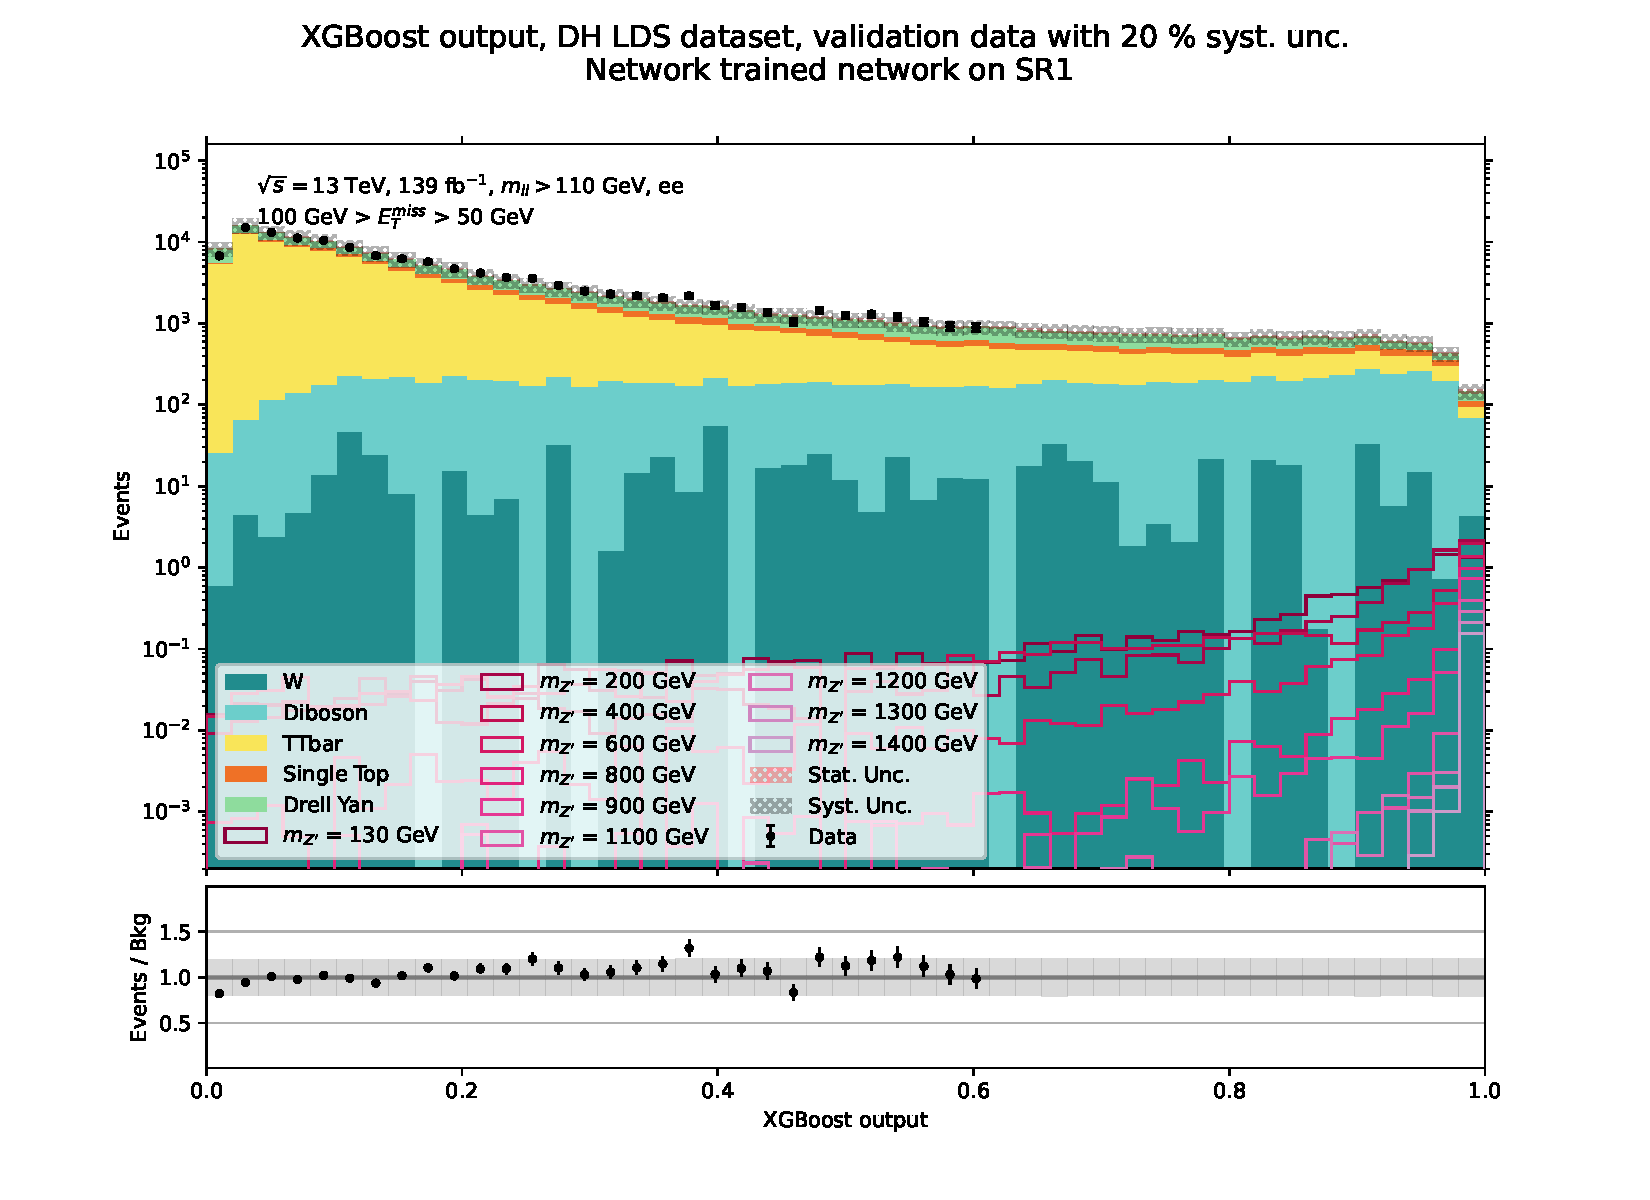
\includegraphics[width=1\textwidth]{XGBoost/Model_independent/50-100/DH_LDS/VAL_ee.pdf}
   \end{subfigure}
   \hfill
   \begin{subfigure}[b]{0.49\textwidth}
      \centering
      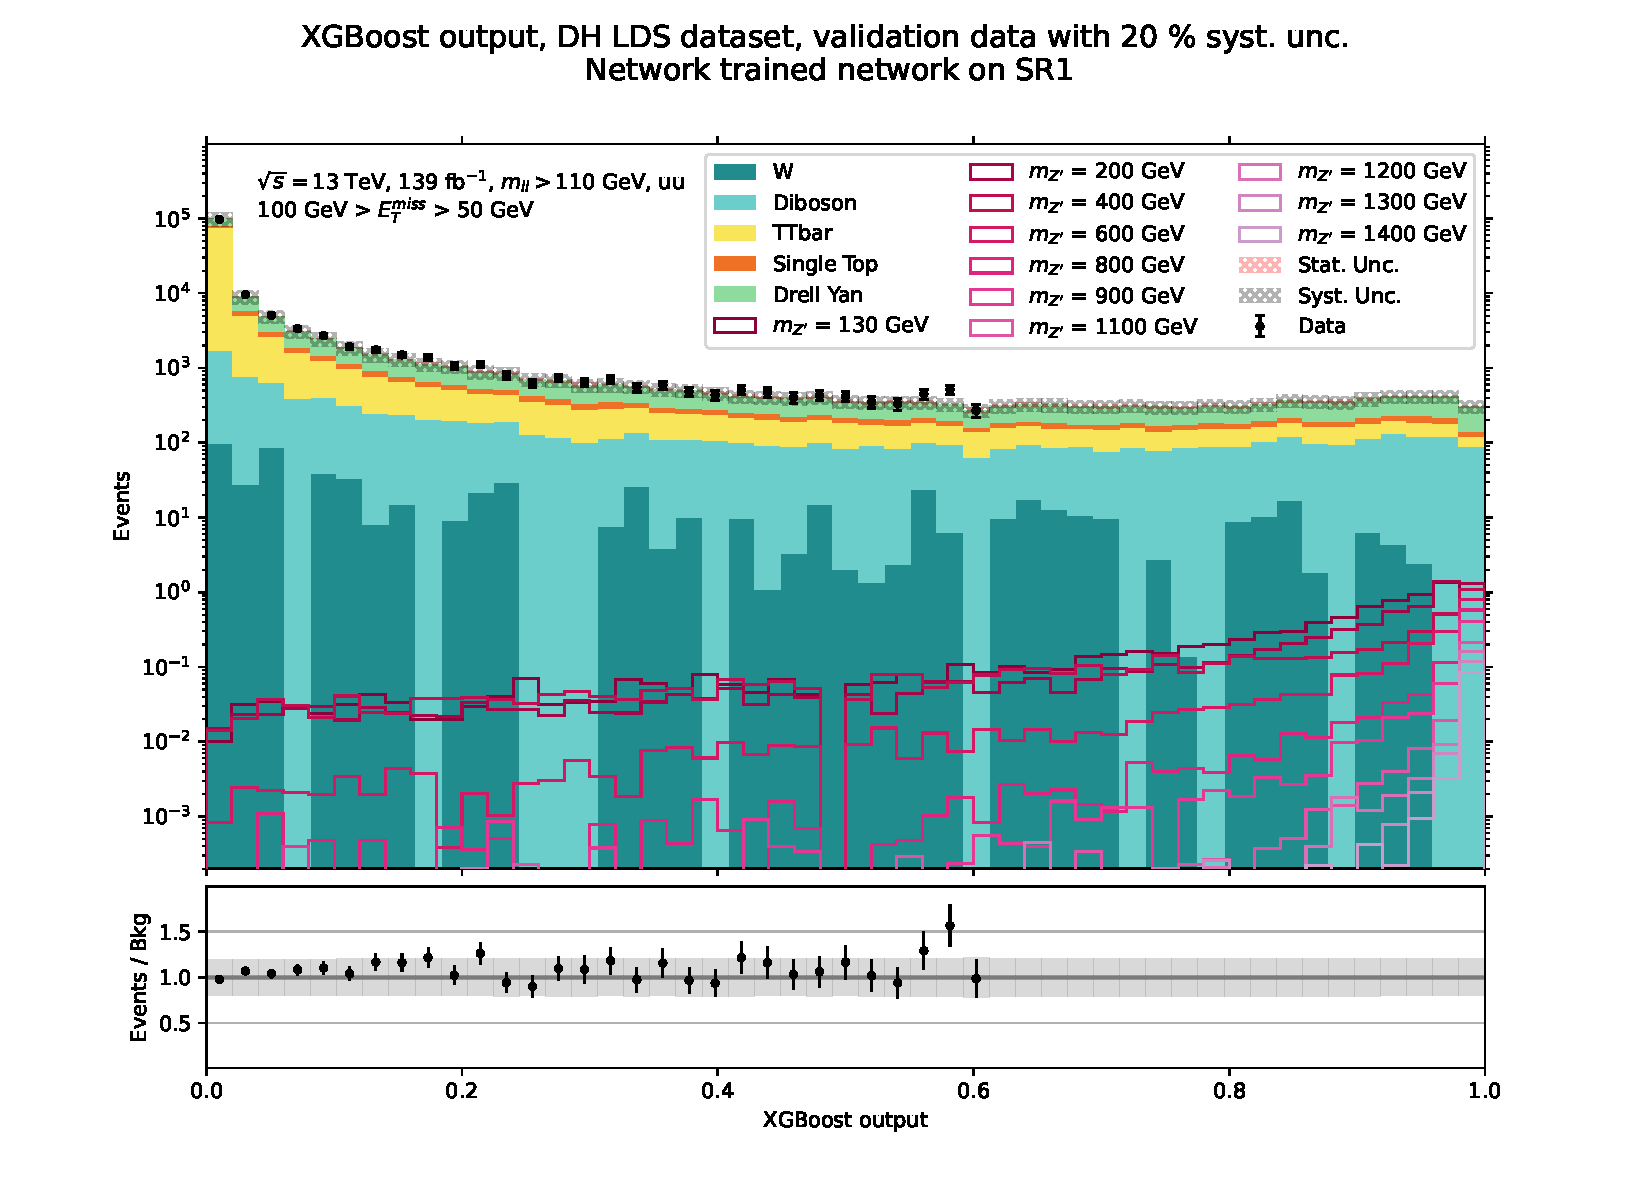
\includegraphics[width=1\textwidth]{XGBoost/Model_independent/50-100/DH_LDS/VAL_uu.pdf}
   \end{subfigure}
   \hfill
   \begin{subfigure}[b]{0.49\textwidth}
      \centering
      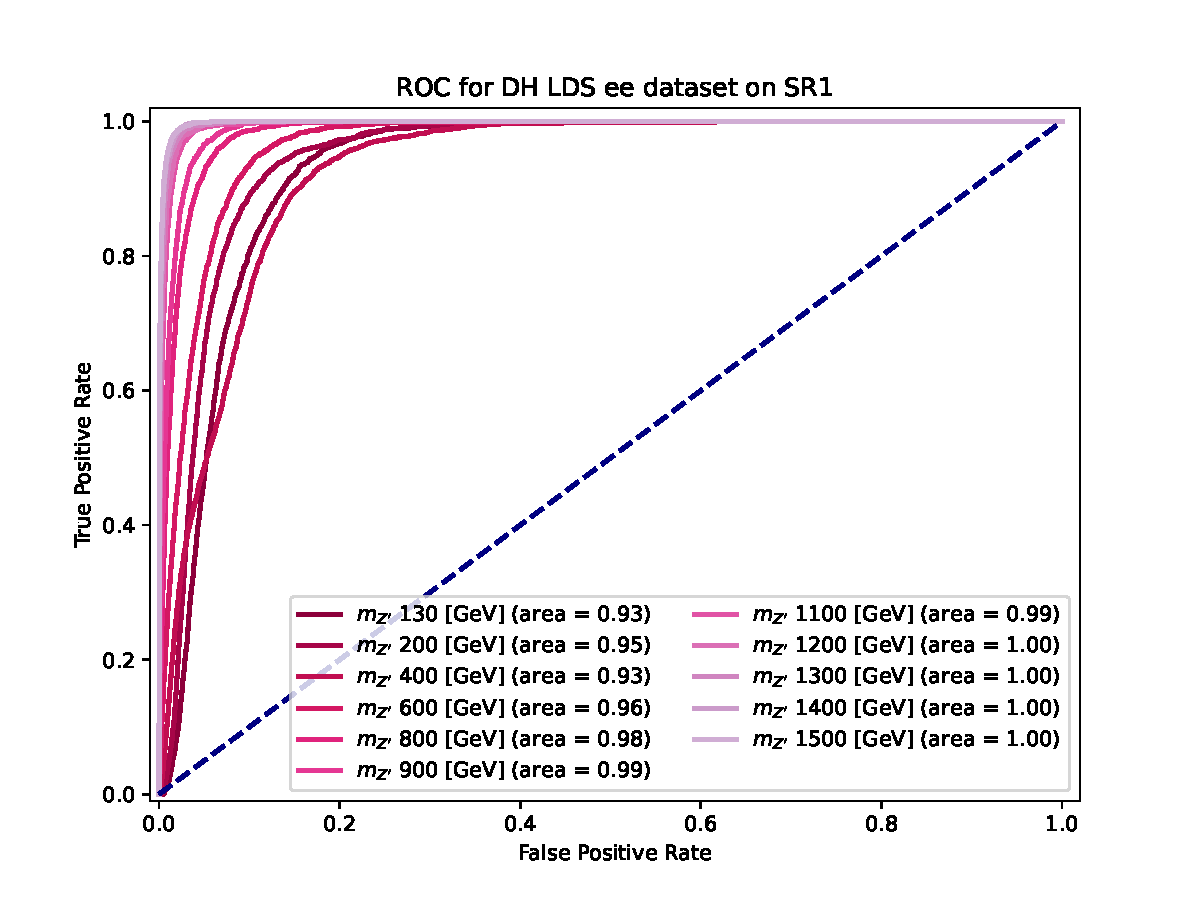
\includegraphics[width=1\textwidth]{XGBoost/Model_independent/50-100/DH_LDS/ROC_ee.pdf}
   \end{subfigure}
   \hfill
   \begin{subfigure}[b]{0.49\textwidth}
      \centering
      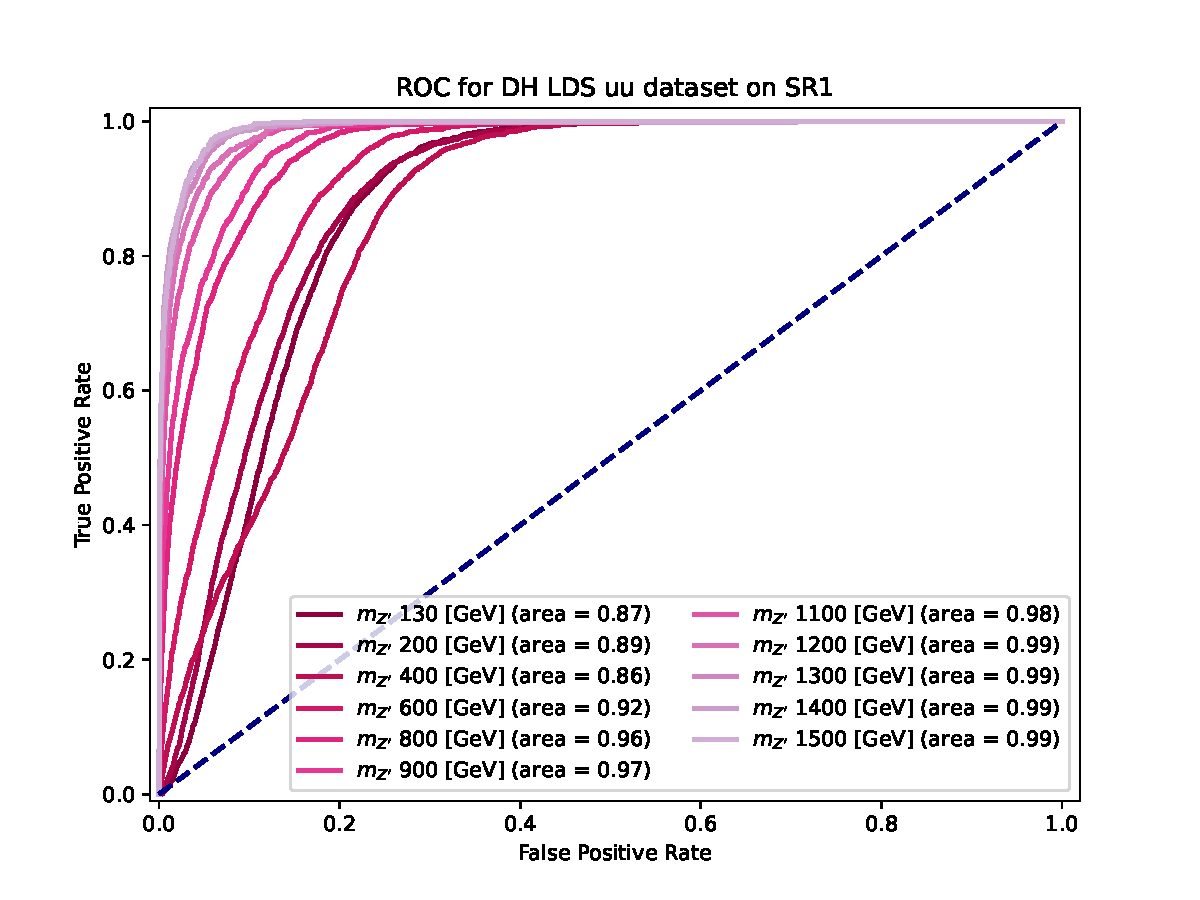
\includegraphics[width=1\textwidth]{XGBoost/Model_independent/50-100/DH_LDS/ROC_uu.pdf}
   \end{subfigure}
   \hfill
	\begin{subfigure}[b]{0.49\textwidth}
      \centering
      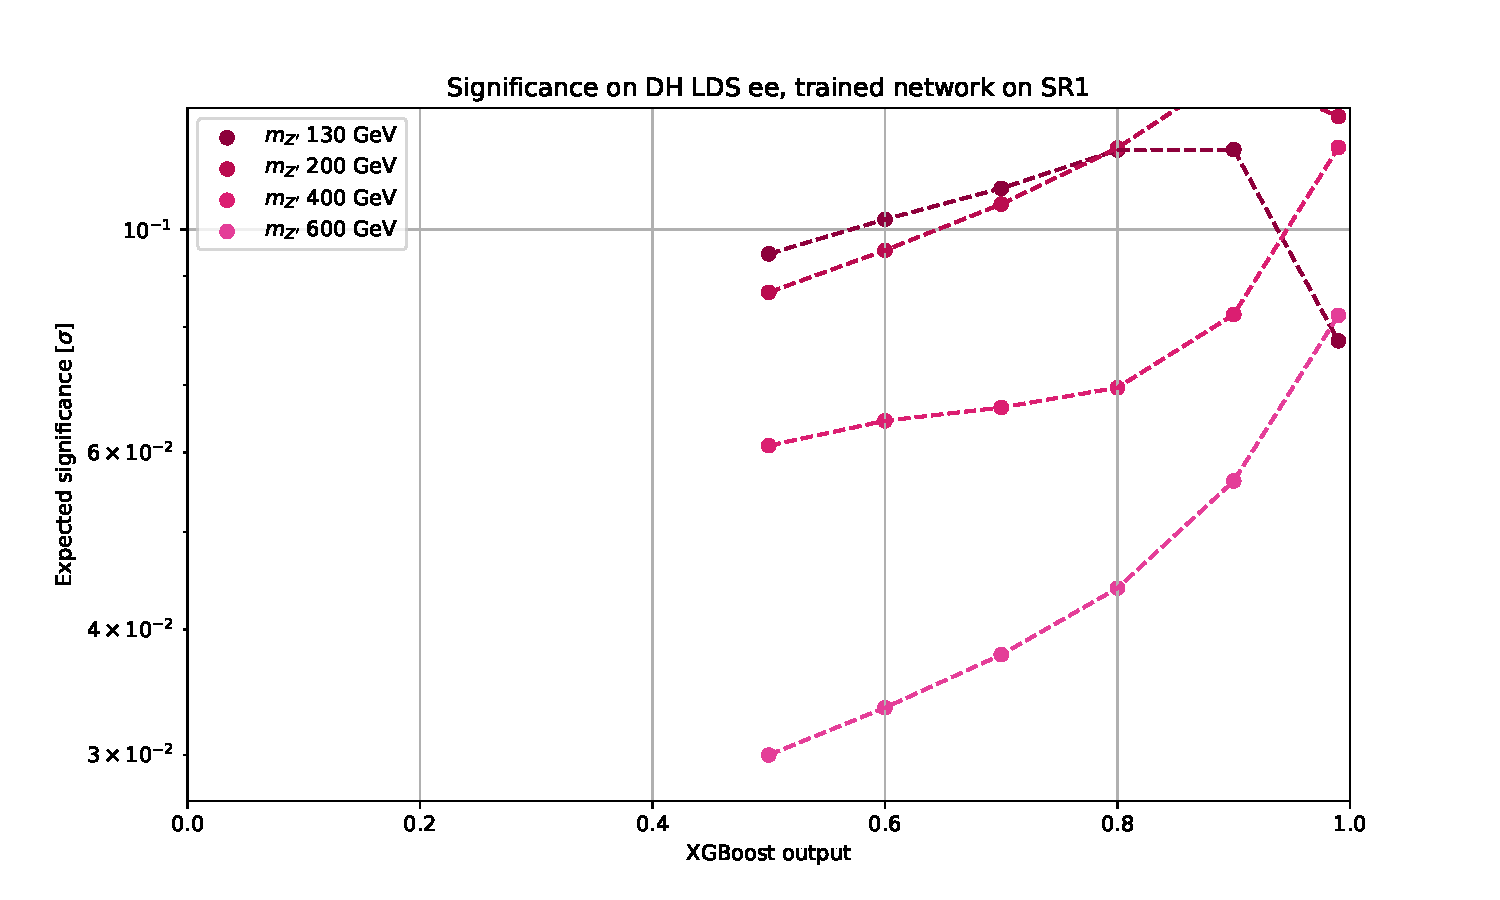
\includegraphics[width=1\textwidth]{XGBoost/Model_independent/50-100/DH_LDS/EXP_SIG_ee.pdf}
   \end{subfigure}
   \hfill
   \begin{subfigure}[b]{0.49\textwidth}
      \centering
      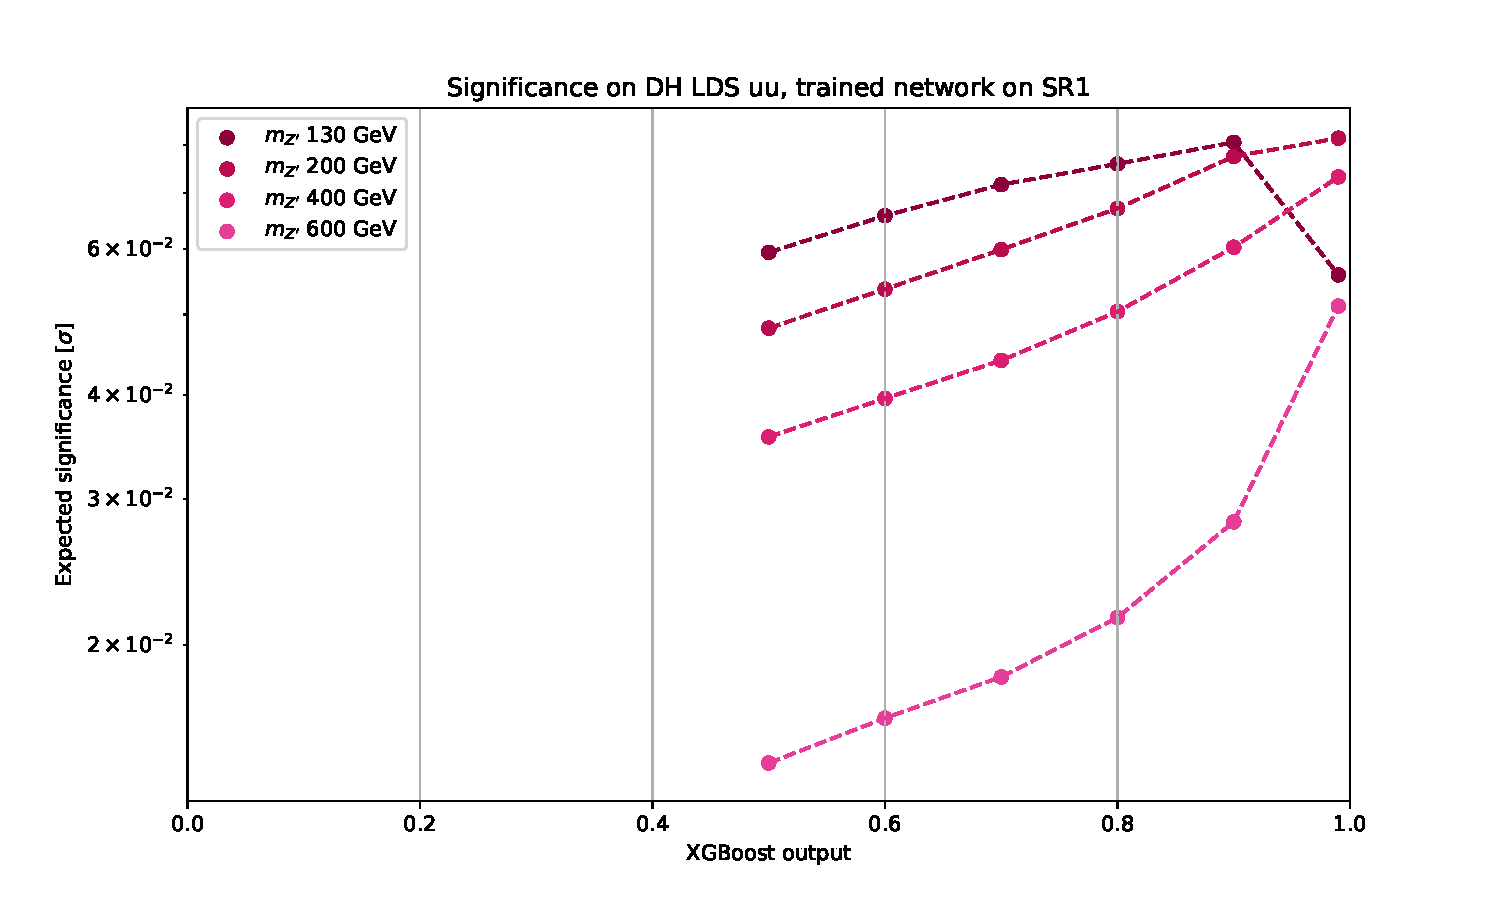
\includegraphics[width=1\textwidth]{XGBoost/Model_independent/50-100/DH_LDS/EXP_SIG_uu.pdf}
   \end{subfigure}
   \caption{XGBoost results for DH LDS model on $ee$ and $\mu\mu$ channel in SR1}\label{fig:DH_LDS_SR1}
\end{figure}

\begin{figure}[!ht]
	\centering
	\begin{subfigure}[b]{0.49\textwidth}
      \centering
      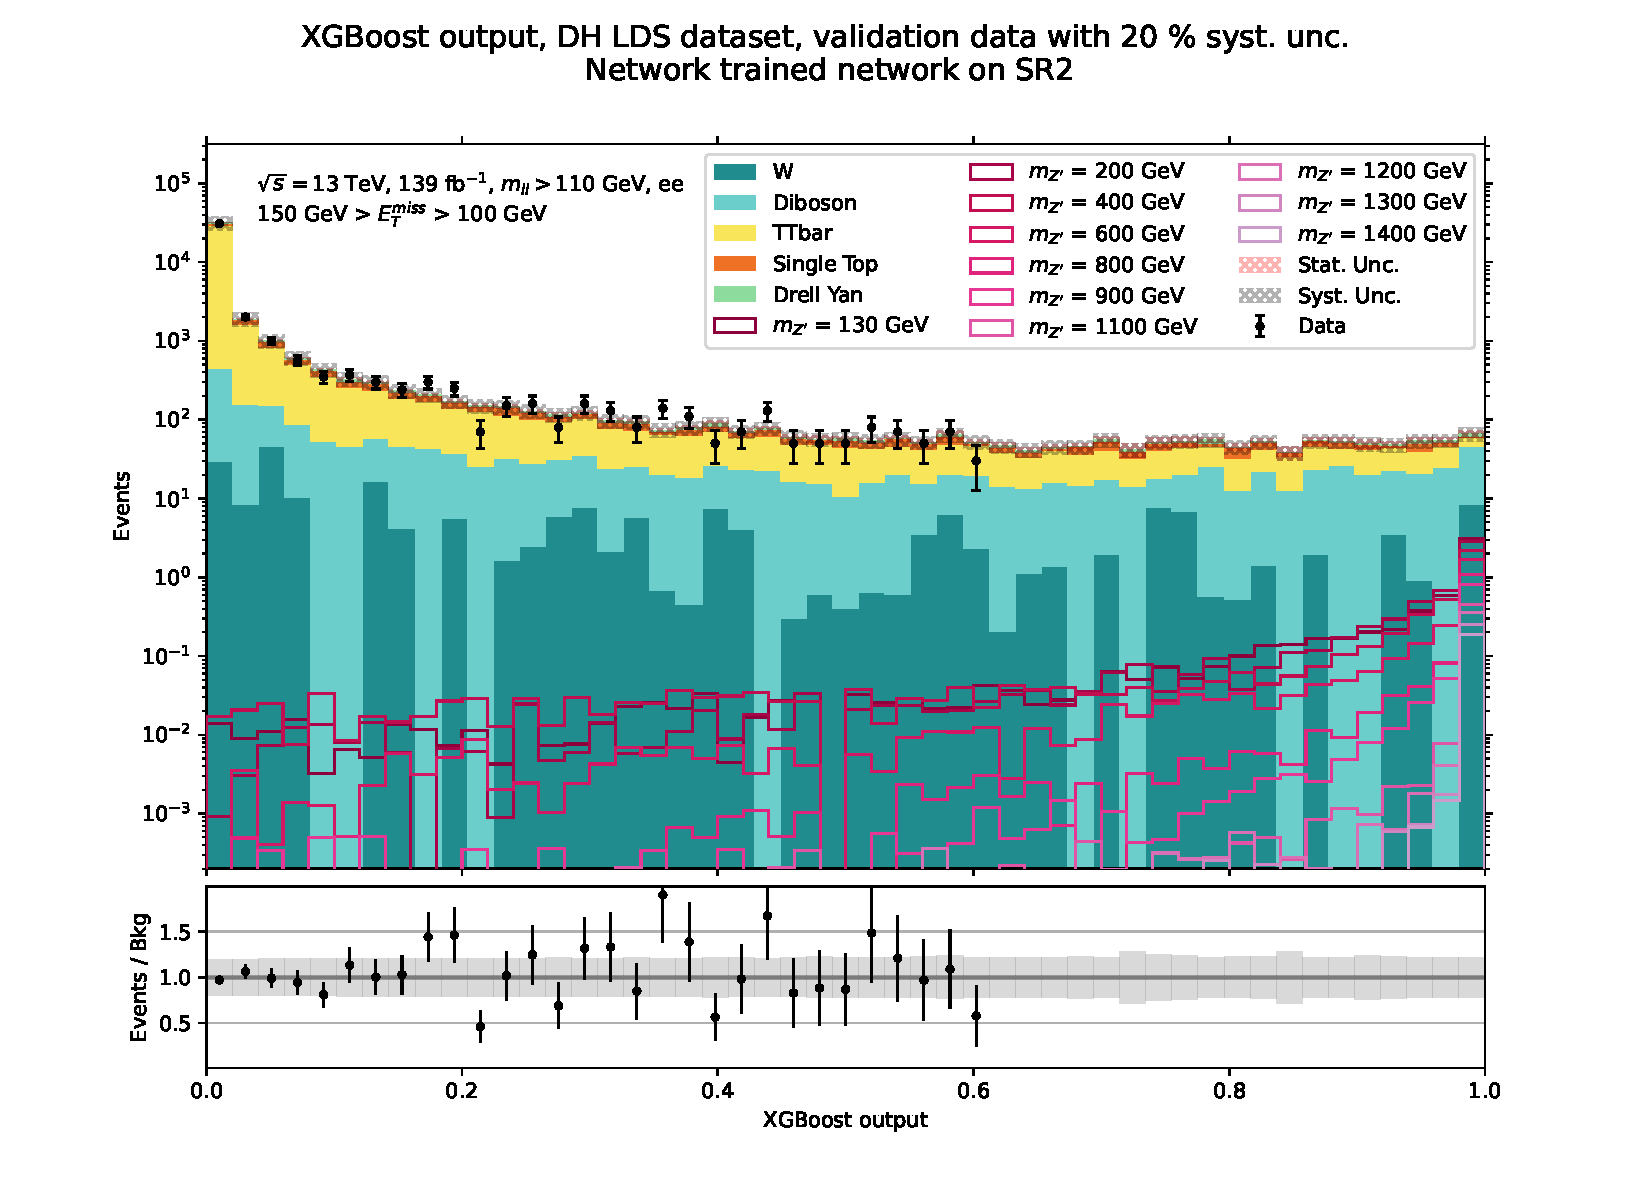
\includegraphics[width=1\textwidth]{XGBoost/Model_independent/100-150/DH_LDS/VAL_ee.pdf}
   \end{subfigure}
   \hfill
   \begin{subfigure}[b]{0.49\textwidth}
      \centering
      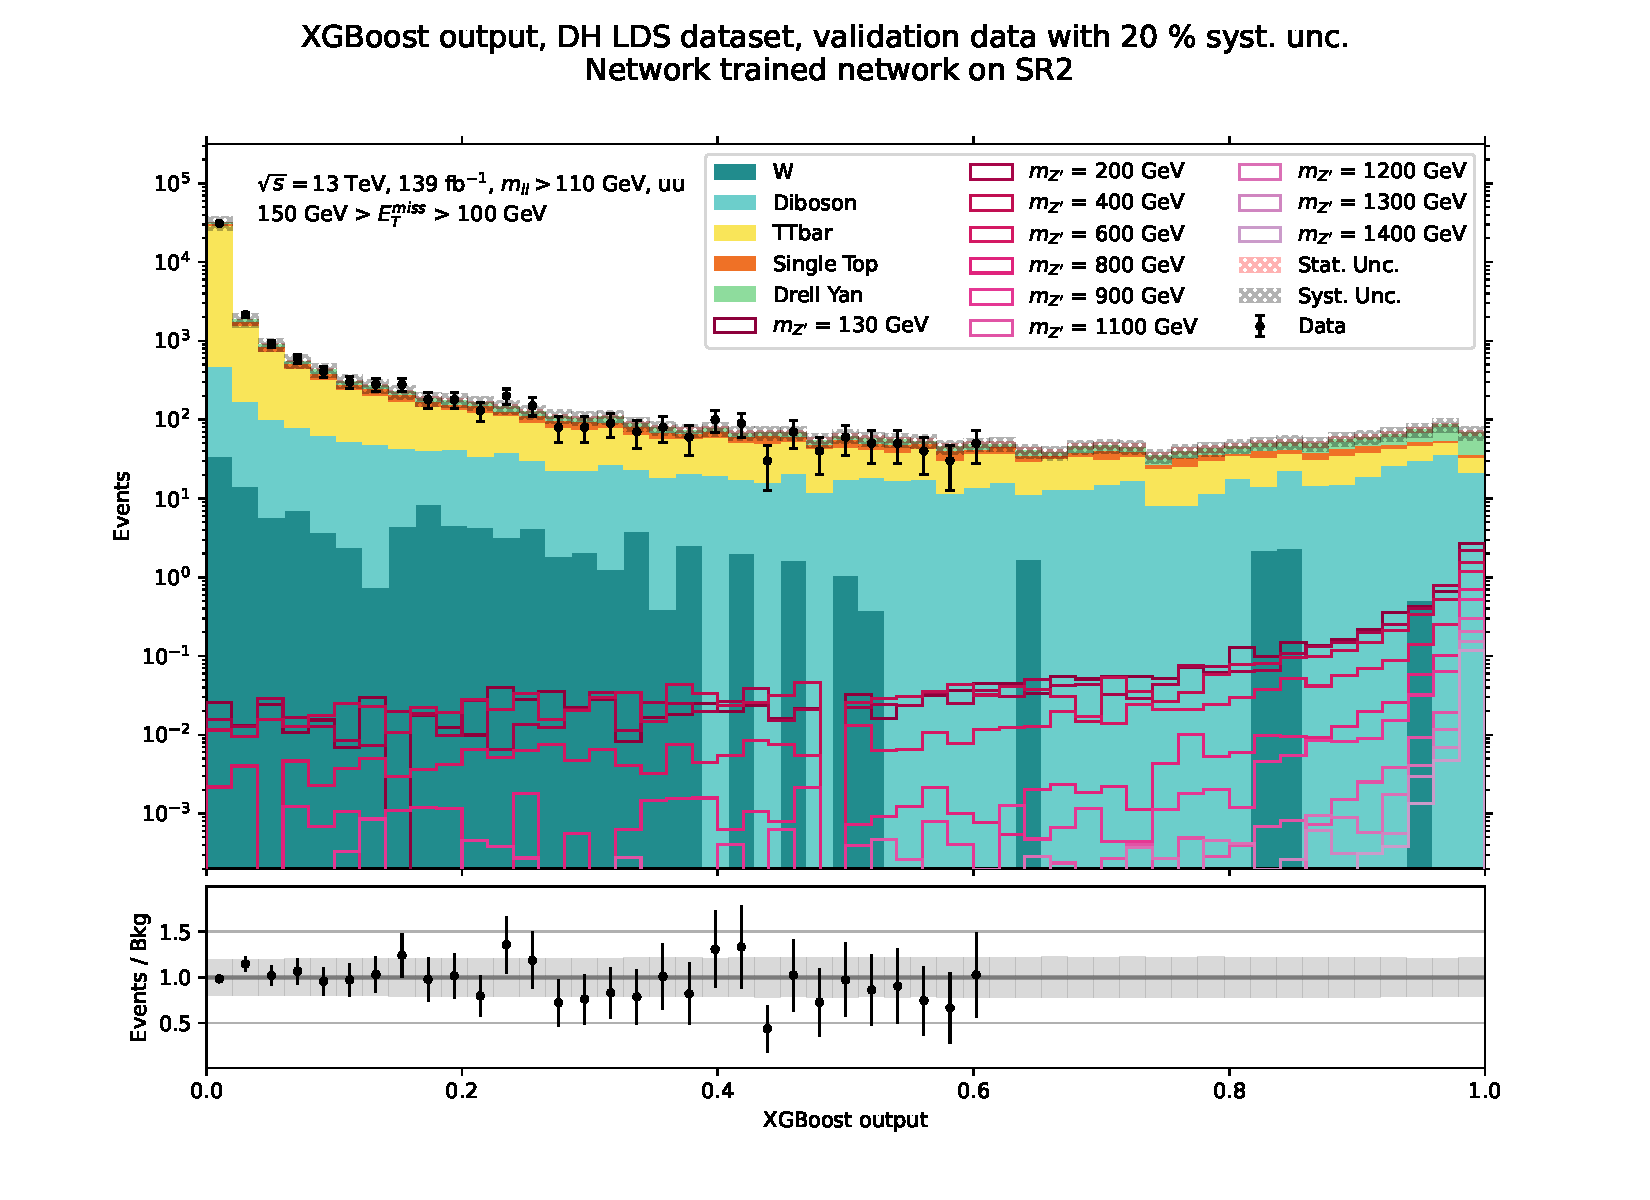
\includegraphics[width=1\textwidth]{XGBoost/Model_independent/100-150/DH_LDS/VAL_uu.pdf}
   \end{subfigure}
   \hfill
   \begin{subfigure}[b]{0.49\textwidth}
      \centering
      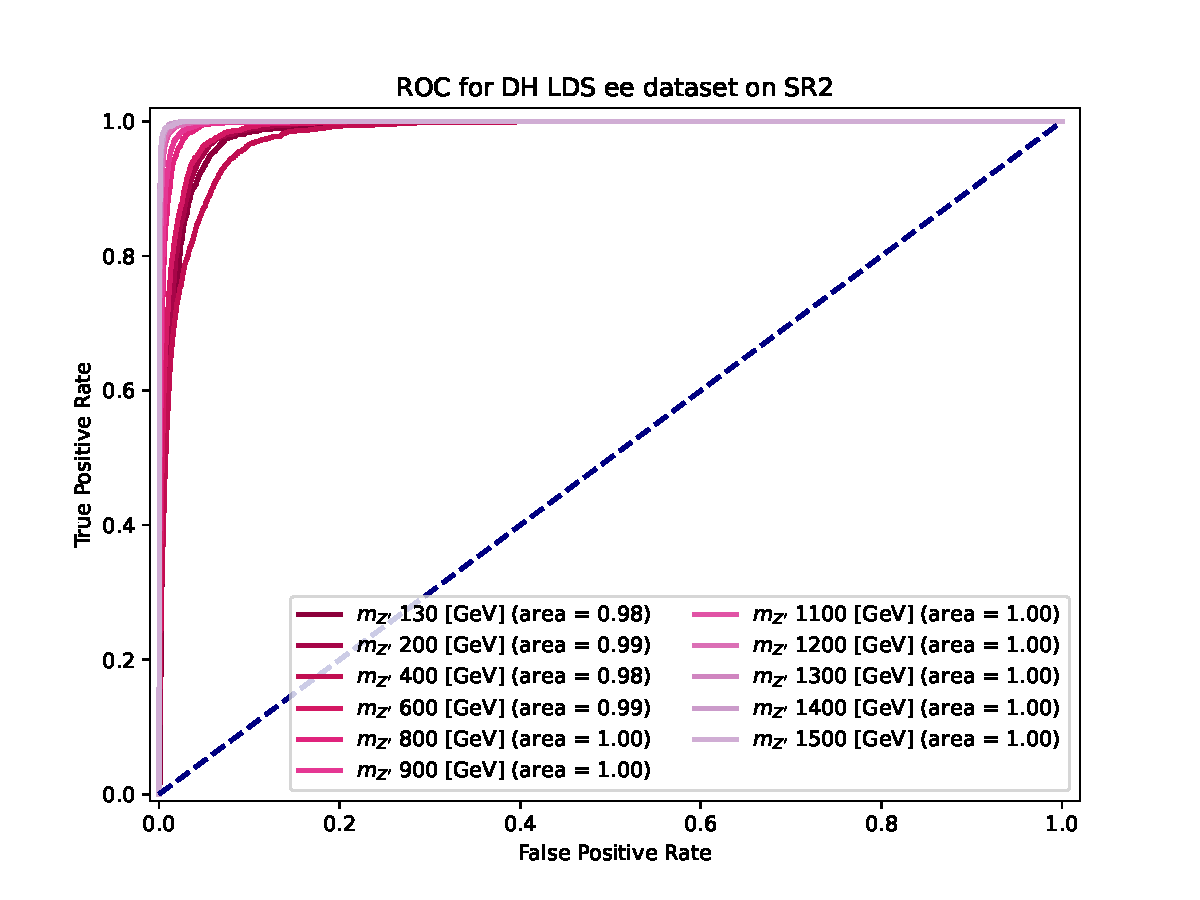
\includegraphics[width=1\textwidth]{XGBoost/Model_independent/100-150/DH_LDS/ROC_ee.pdf}
   \end{subfigure}
   \hfill
   \begin{subfigure}[b]{0.49\textwidth}
      \centering
      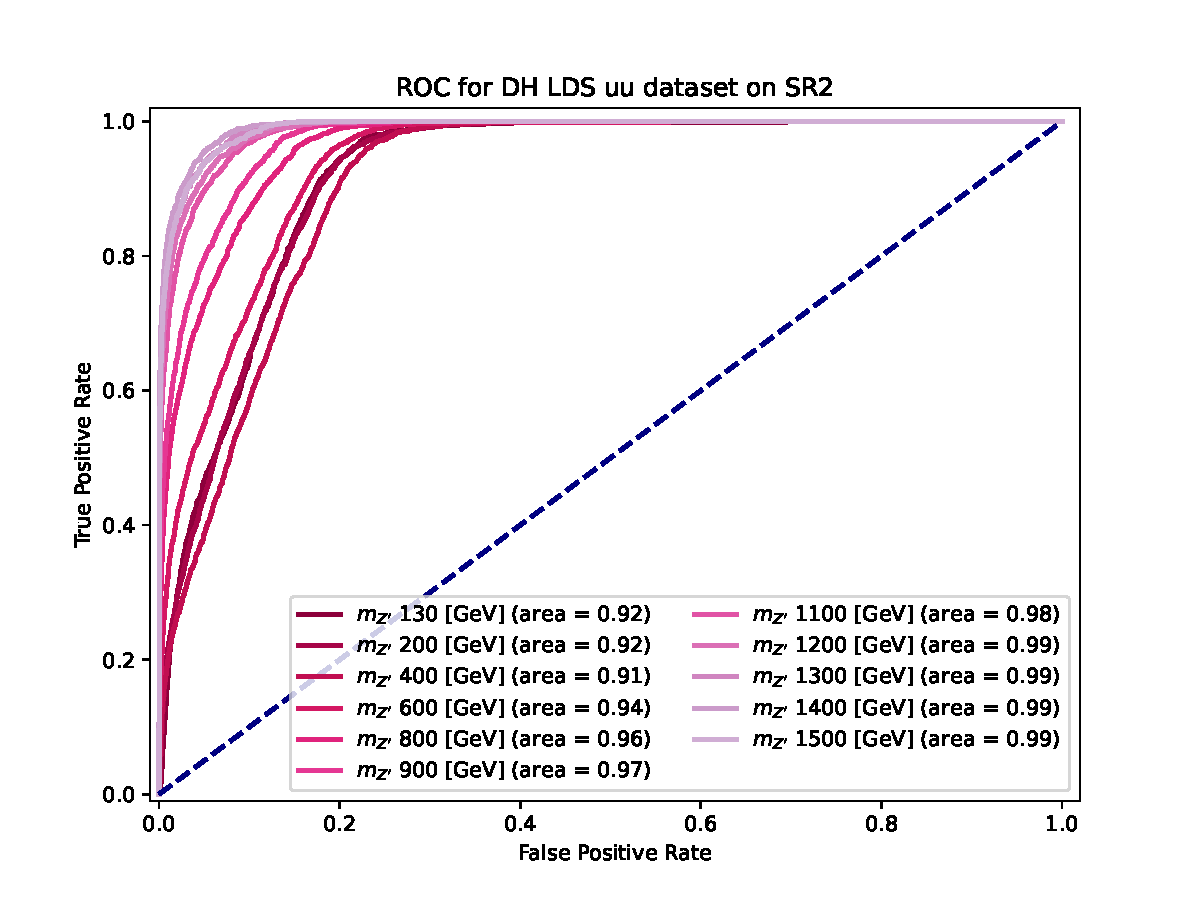
\includegraphics[width=1\textwidth]{XGBoost/Model_independent/100-150/DH_LDS/ROC_uu.pdf}
   \end{subfigure}
   \hfill
	\begin{subfigure}[b]{0.49\textwidth}
      \centering
      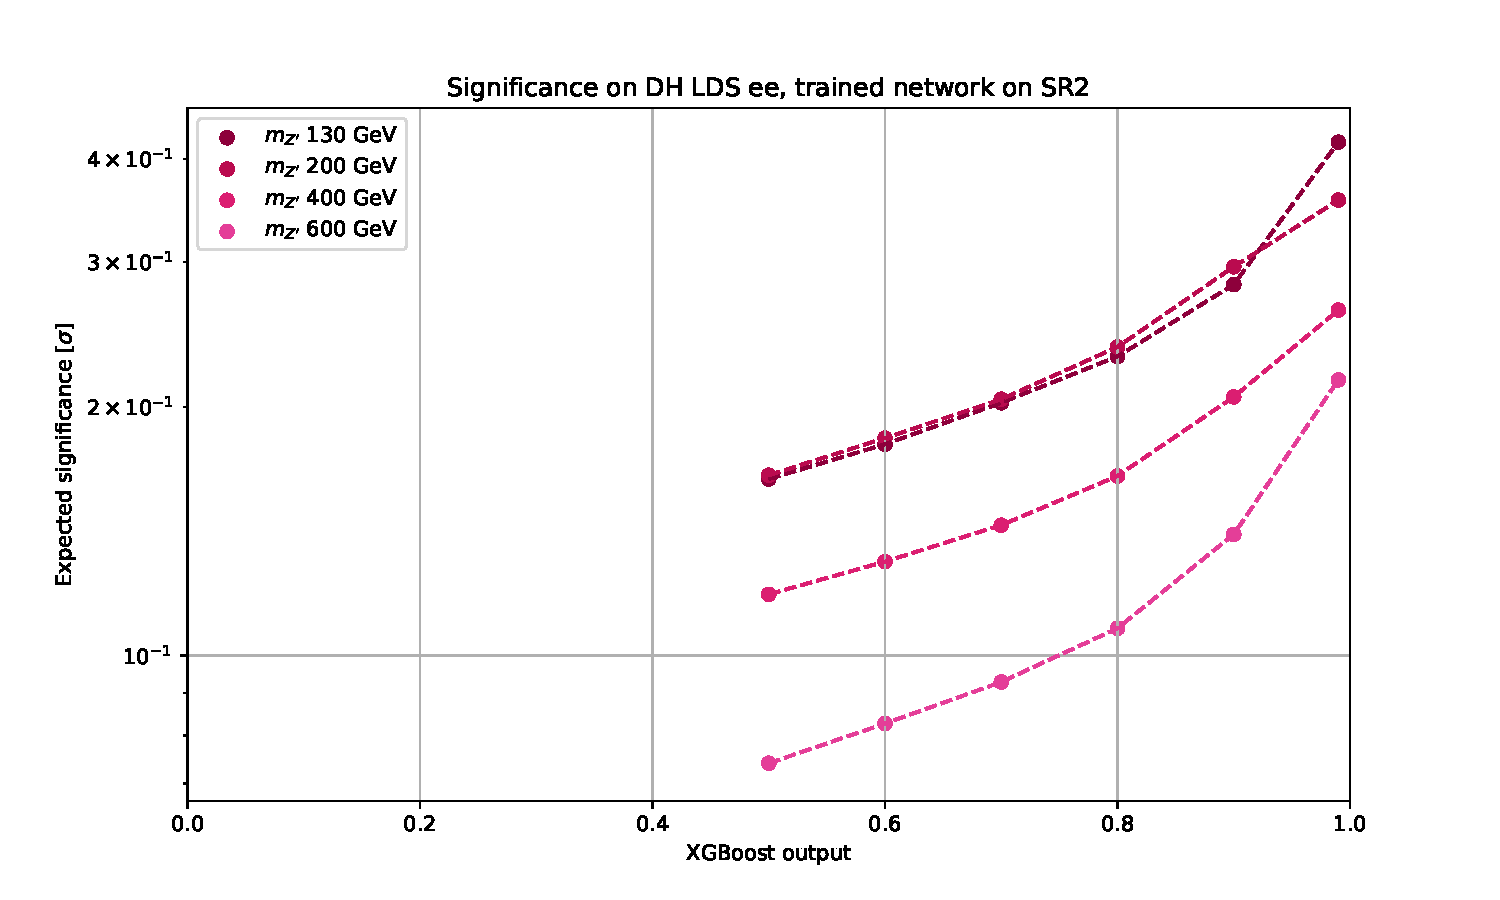
\includegraphics[width=1\textwidth]{XGBoost/Model_independent/100-150/DH_LDS/EXP_SIG_ee.pdf}
   \end{subfigure}
   \hfill
   \begin{subfigure}[b]{0.49\textwidth}
      \centering
      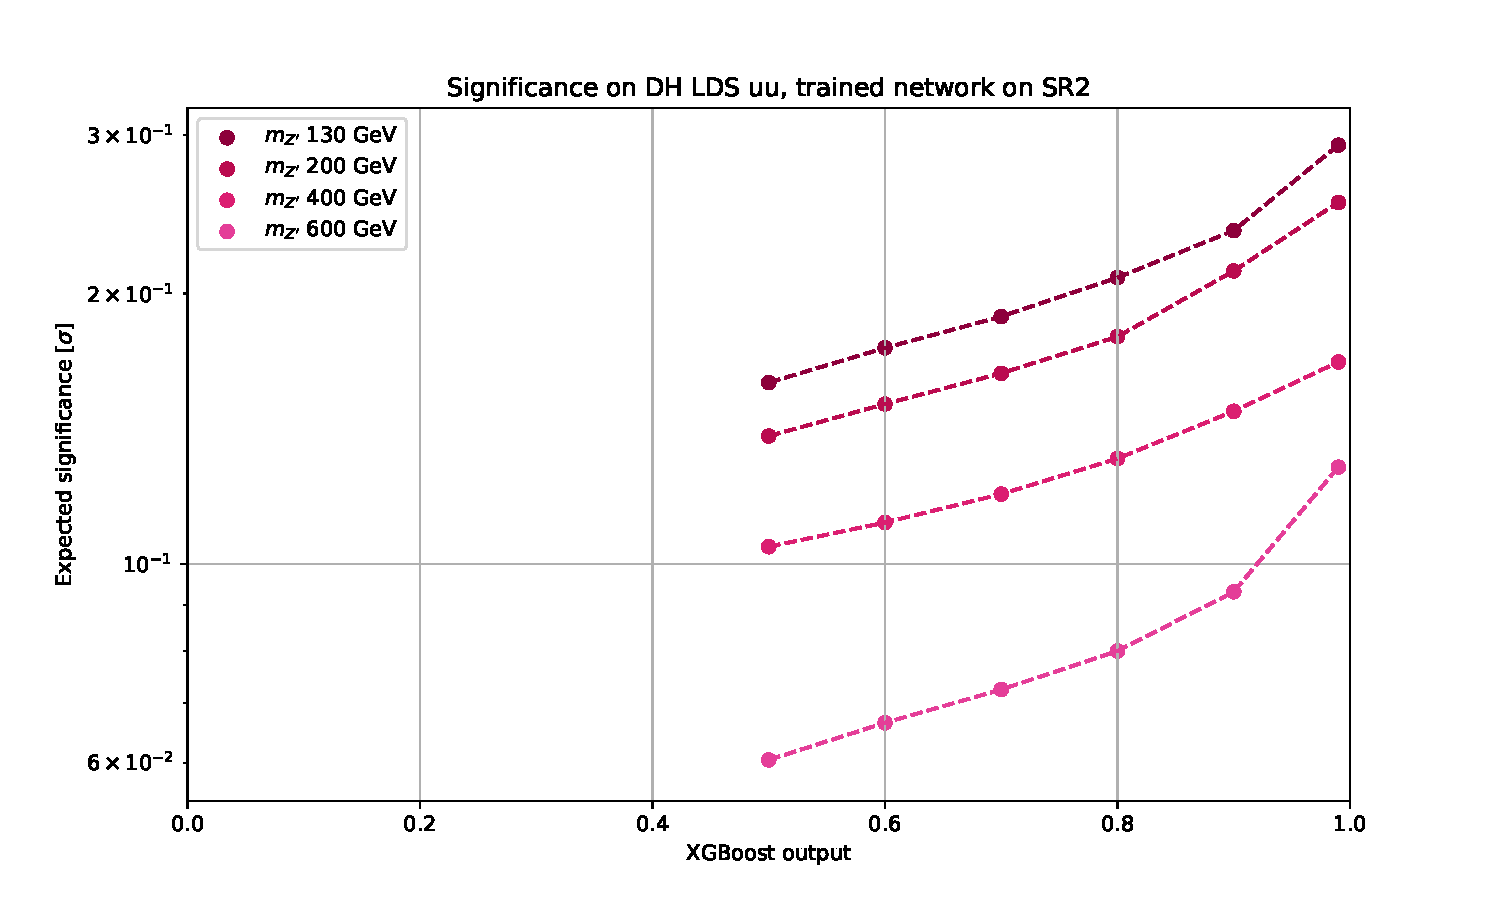
\includegraphics[width=1\textwidth]{XGBoost/Model_independent/100-150/DH_LDS/EXP_SIG_uu.pdf}
   \end{subfigure}
   \caption{XGBoost results for DH LDS model on $ee$ and $\mu\mu$ channel in SR2}\label{fig:DH_LDS_SR2}
\end{figure}

\begin{figure}[!ht]
	\centering
	\begin{subfigure}[b]{0.49\textwidth}
      \centering
      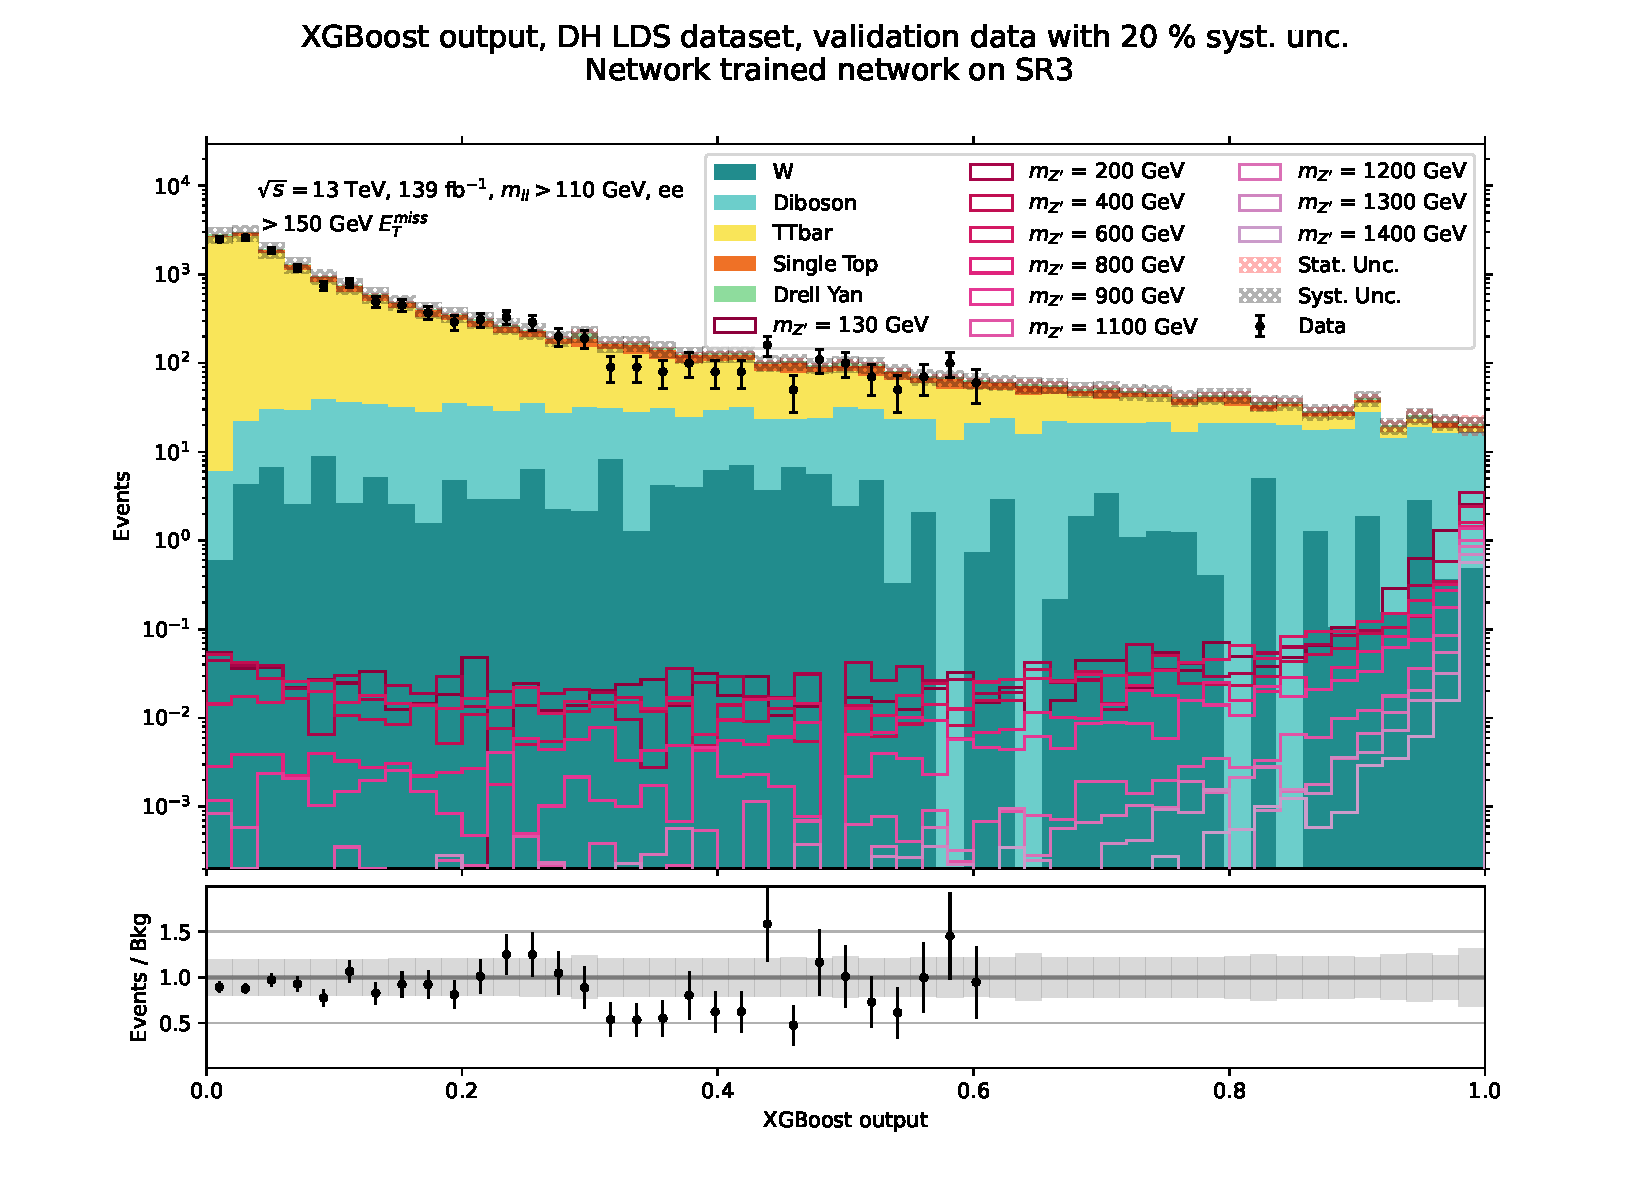
\includegraphics[width=1\textwidth]{XGBoost/Model_independent/150/DH_LDS/VAL_ee.pdf}
   \end{subfigure}
   \hfill
   \begin{subfigure}[b]{0.49\textwidth}
      \centering
      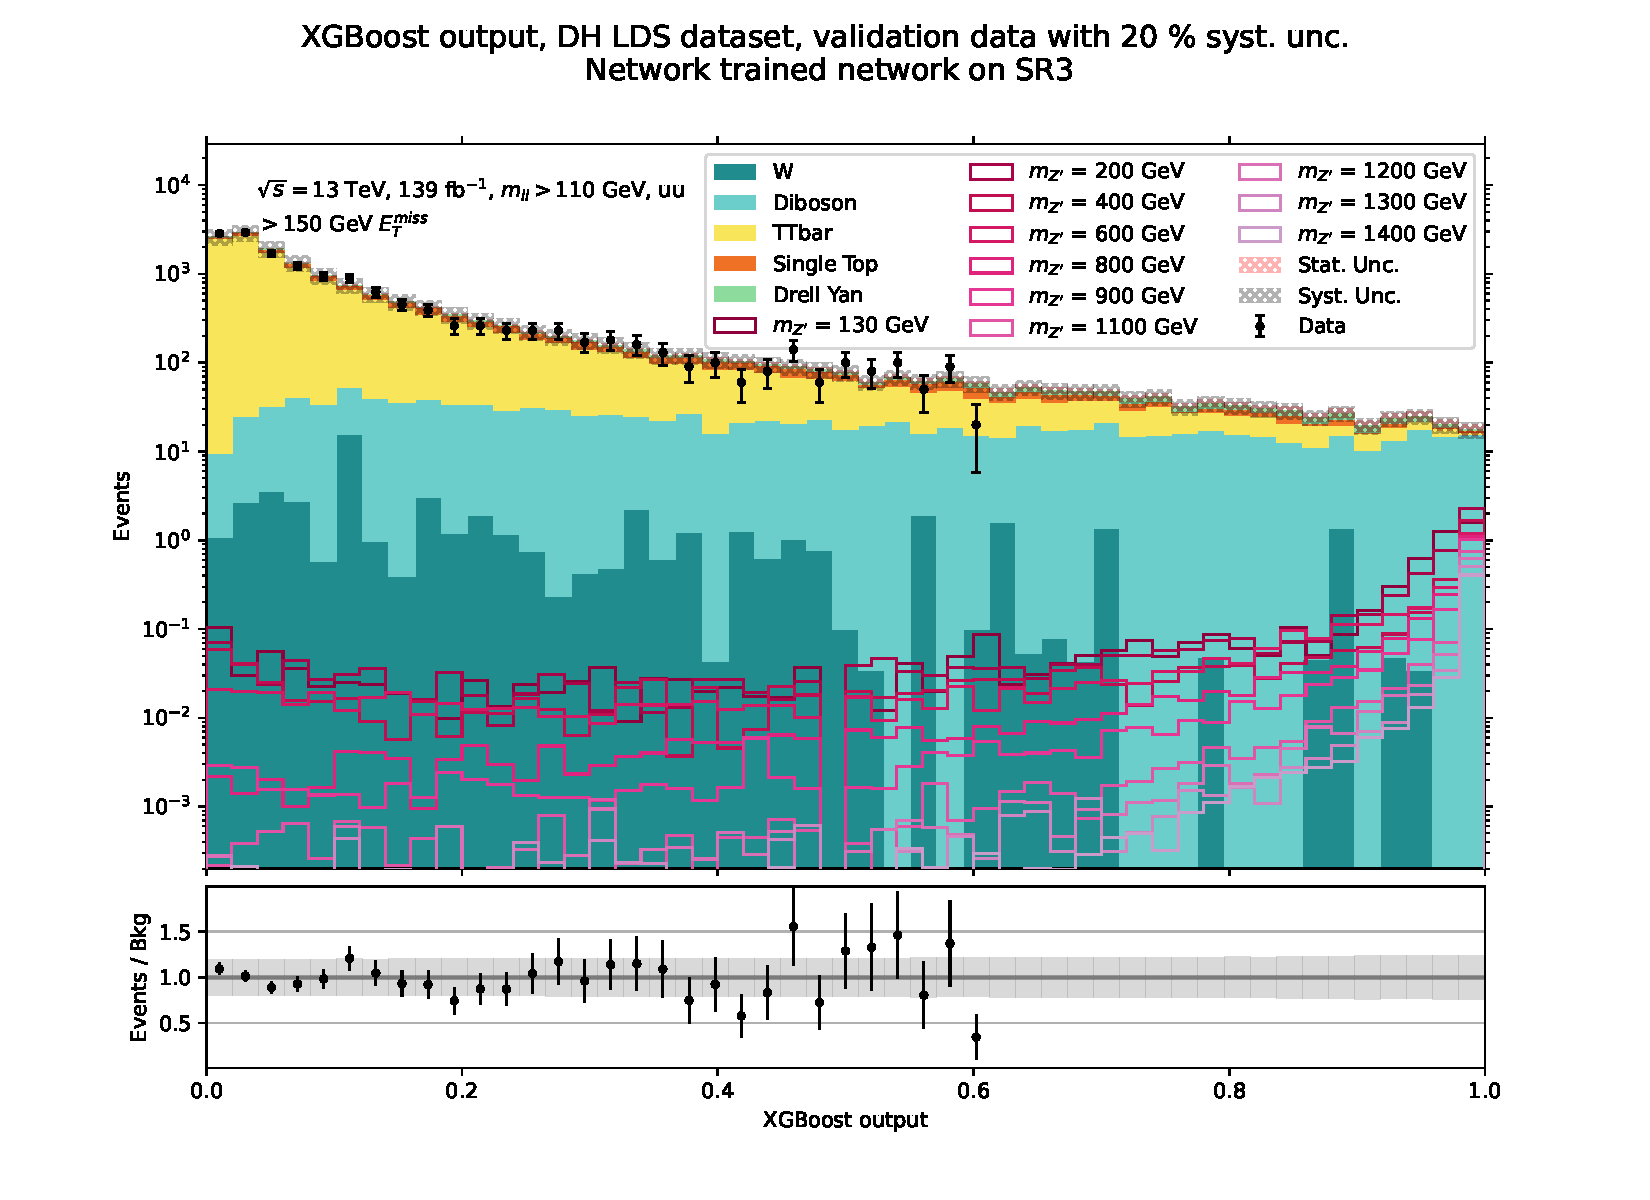
\includegraphics[width=1\textwidth]{XGBoost/Model_independent/150/DH_LDS/VAL_uu.pdf}
   \end{subfigure}
   \hfill
   \begin{subfigure}[b]{0.49\textwidth}
      \centering
      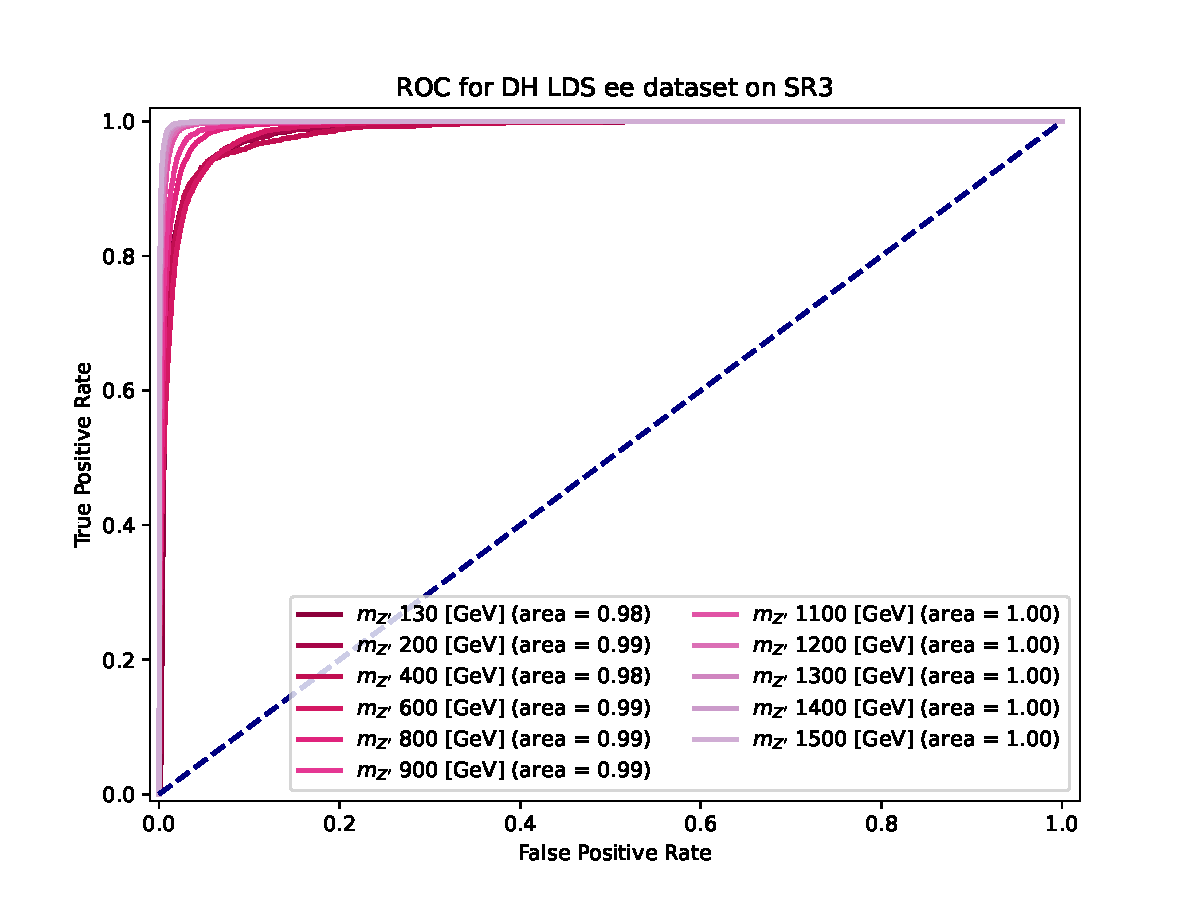
\includegraphics[width=1\textwidth]{XGBoost/Model_independent/150/DH_LDS/ROC_ee.pdf}
   \end{subfigure}
   \hfill
   \begin{subfigure}[b]{0.49\textwidth}
      \centering
      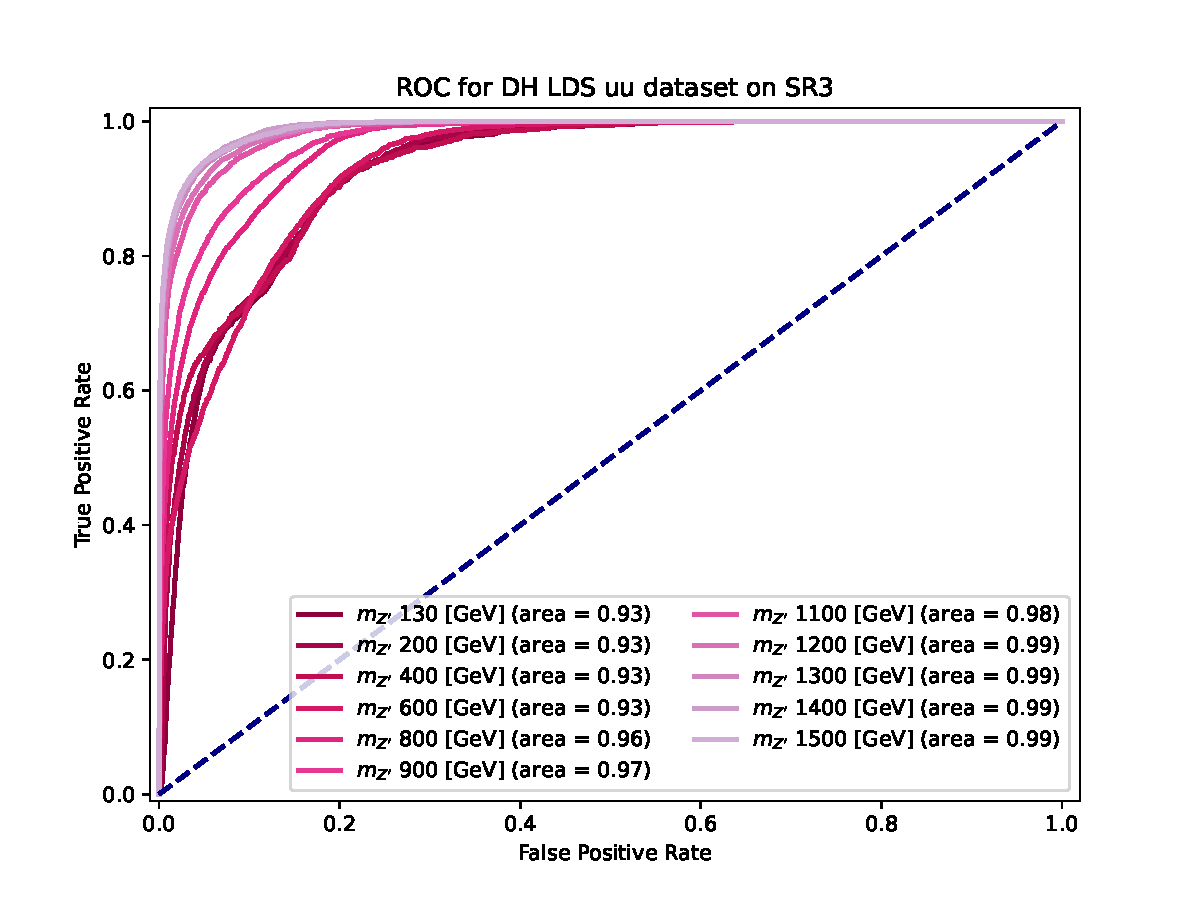
\includegraphics[width=1\textwidth]{XGBoost/Model_independent/150/DH_LDS/ROC_uu.pdf}
   \end{subfigure}
   \hfill
	\begin{subfigure}[b]{0.49\textwidth}
      \centering
      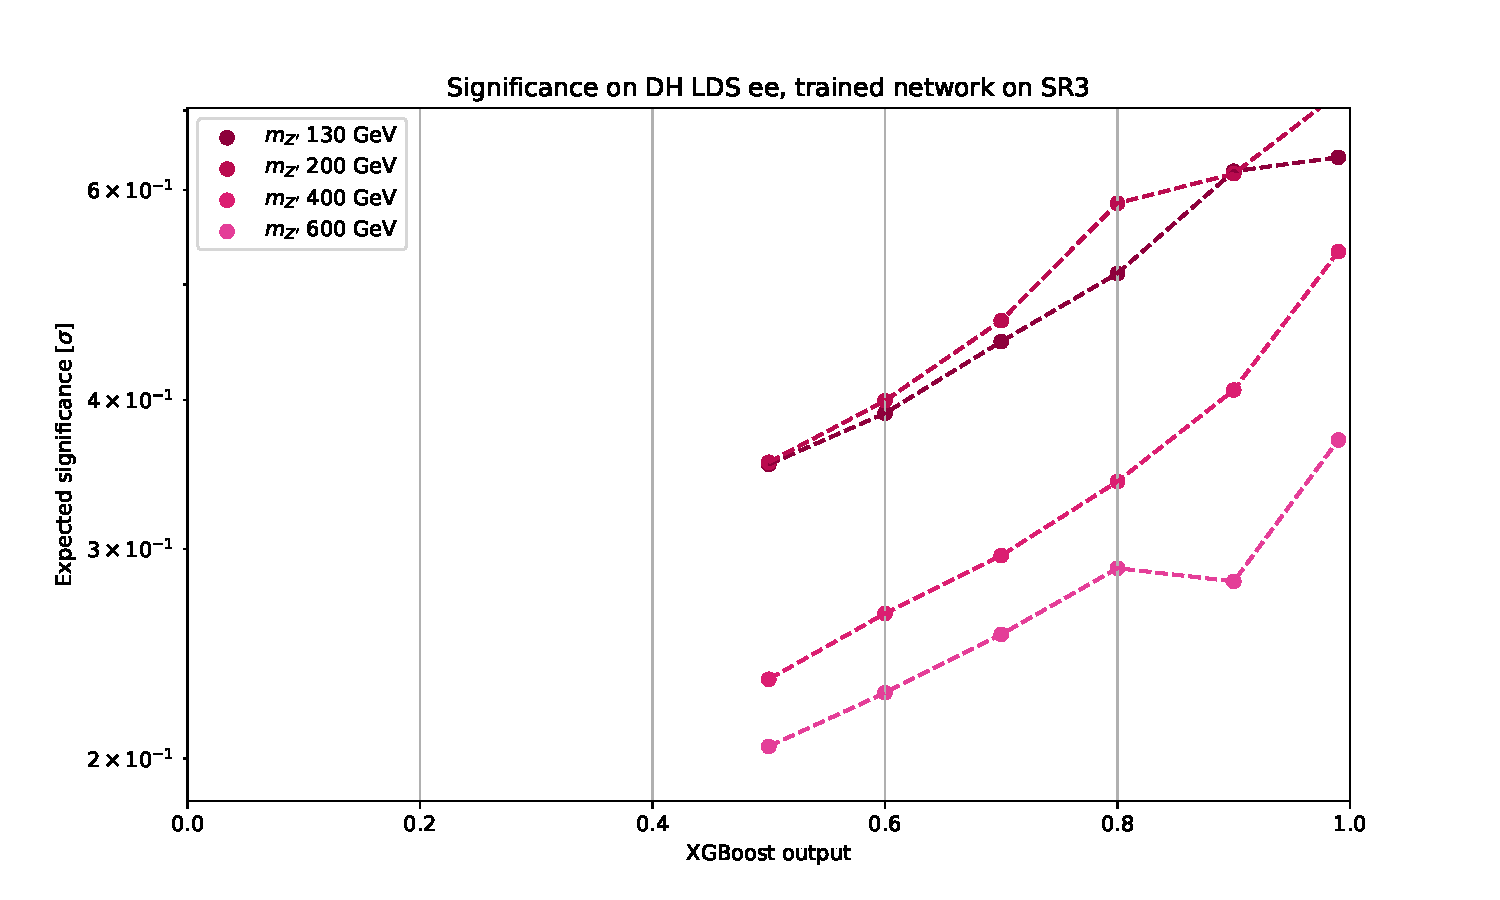
\includegraphics[width=1\textwidth]{XGBoost/Model_independent/150/DH_LDS/EXP_SIG_ee.pdf}
   \end{subfigure}
   \hfill
   \begin{subfigure}[b]{0.49\textwidth}
      \centering
      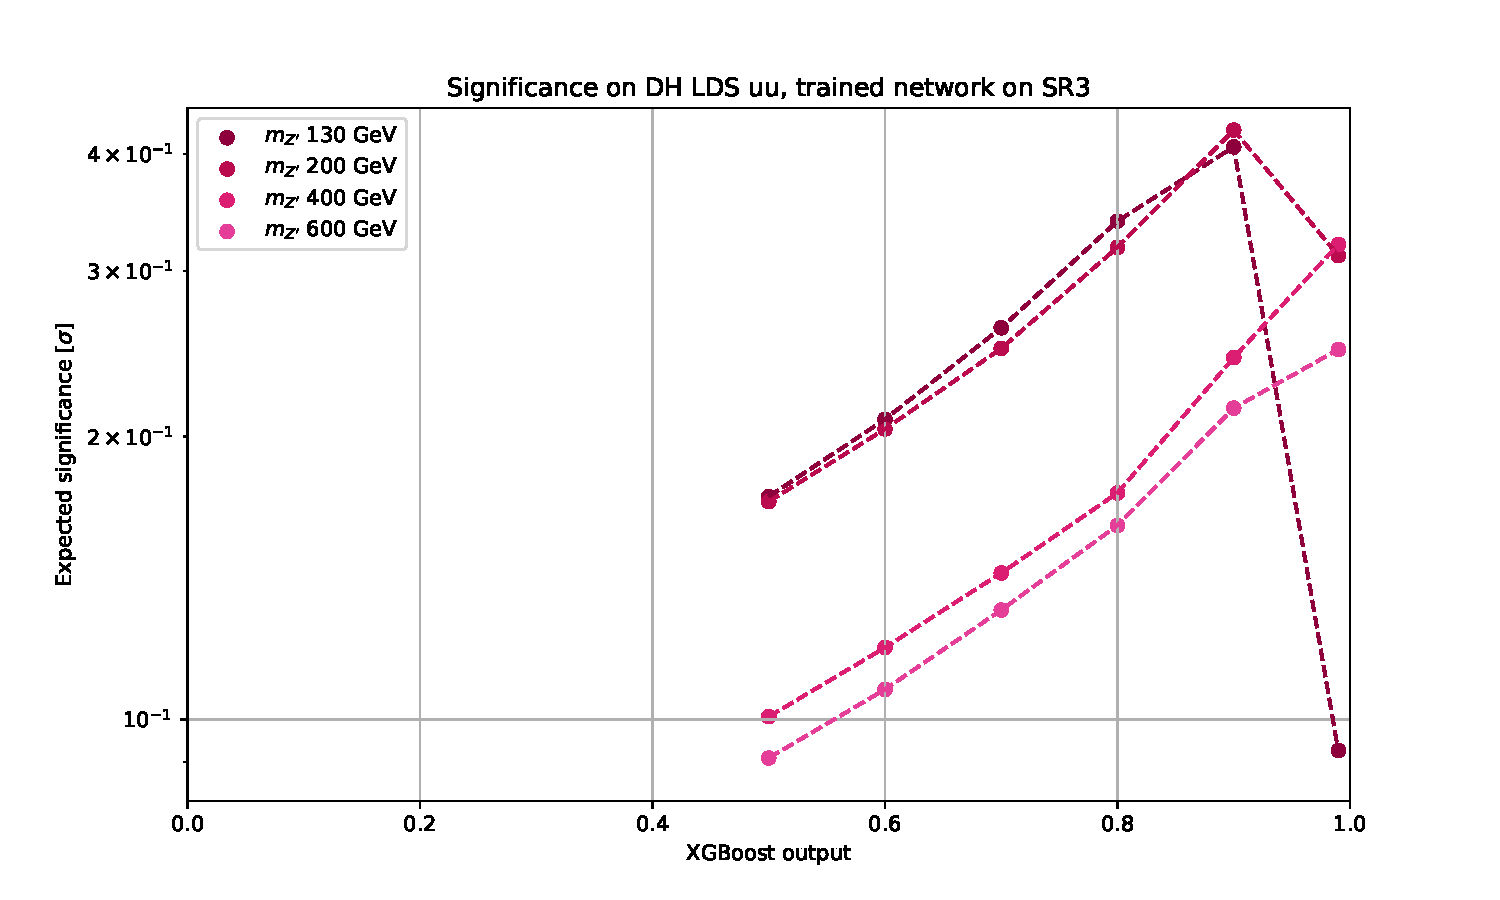
\includegraphics[width=1\textwidth]{XGBoost/Model_independent/150/DH_LDS/EXP_SIG_uu.pdf}
   \end{subfigure}
   \caption{XGBoost results for DH LDS model on $ee$ and $\mu\mu$ channel in SR3}\label{fig:DH_LDS_SR3}
\end{figure}

\begin{figure}[!ht]
	\centering
	\begin{subfigure}[b]{0.49\textwidth}
      \centering
      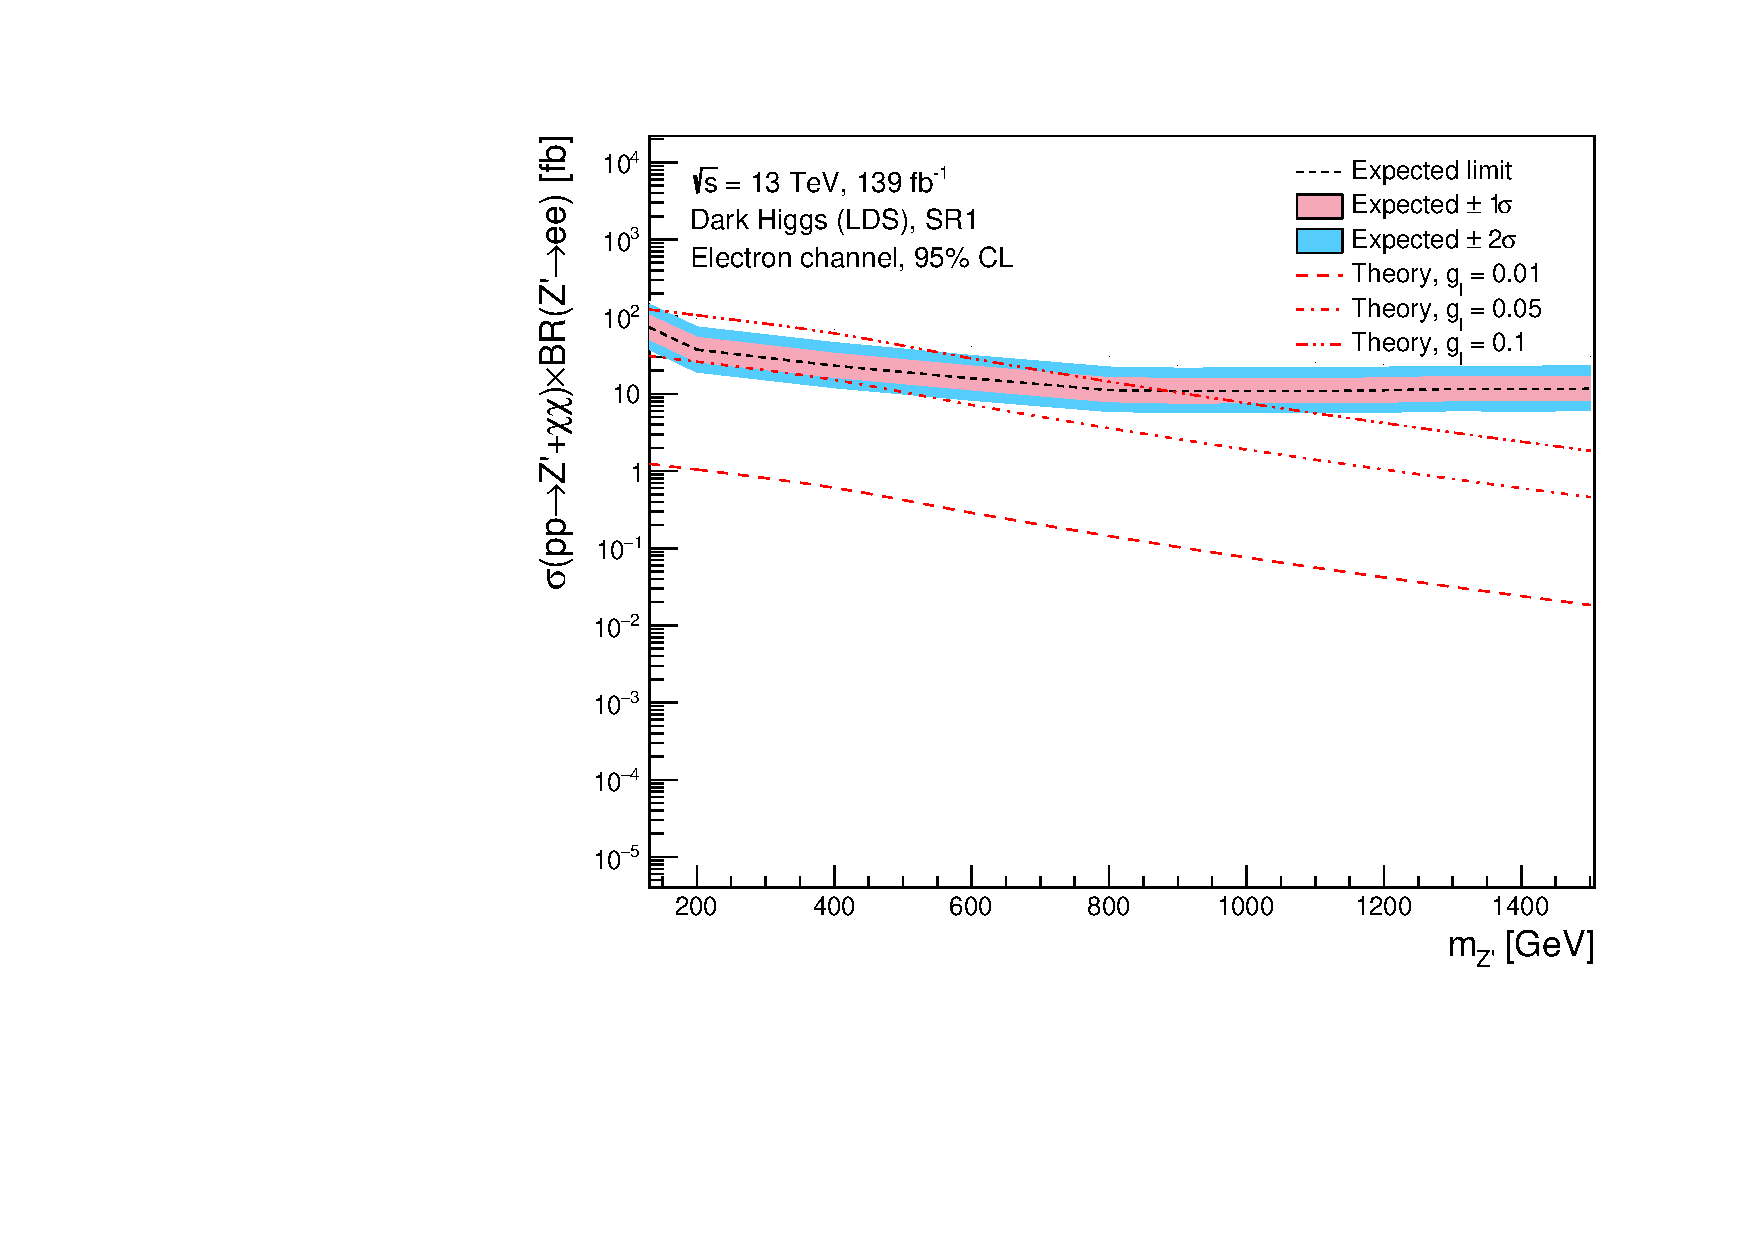
\includegraphics[width=1\textwidth]{Limits/Model_independent/50-100/DH_LDS/mass_exclusion_ee.pdf}
   \end{subfigure}
   \hfill
   \begin{subfigure}[b]{0.49\textwidth}
      \centering
      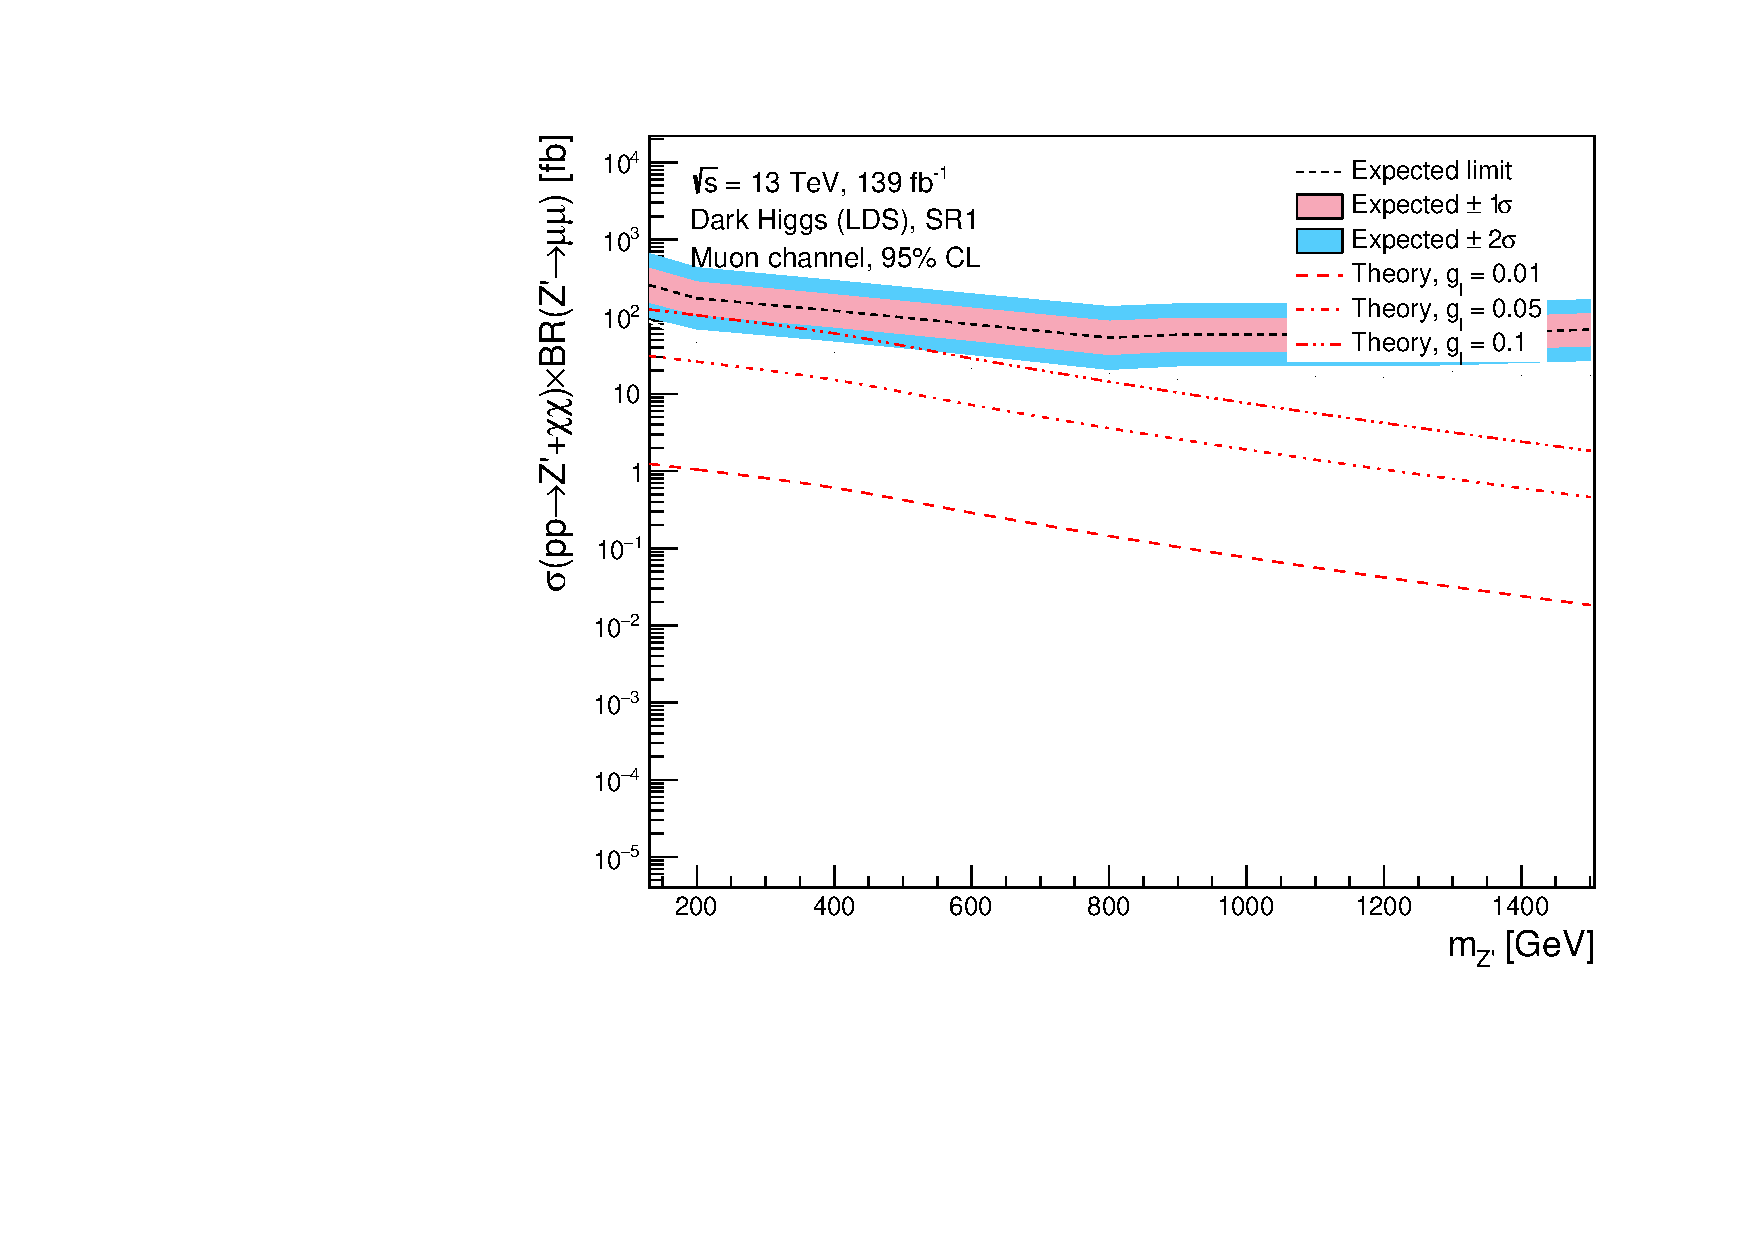
\includegraphics[width=1\textwidth]{Limits/Model_independent/50-100/DH_LDS/mass_exclusion_uu.pdf}
   \end{subfigure}
   \hfill
   \begin{subfigure}[b]{0.49\textwidth}
      \centering
      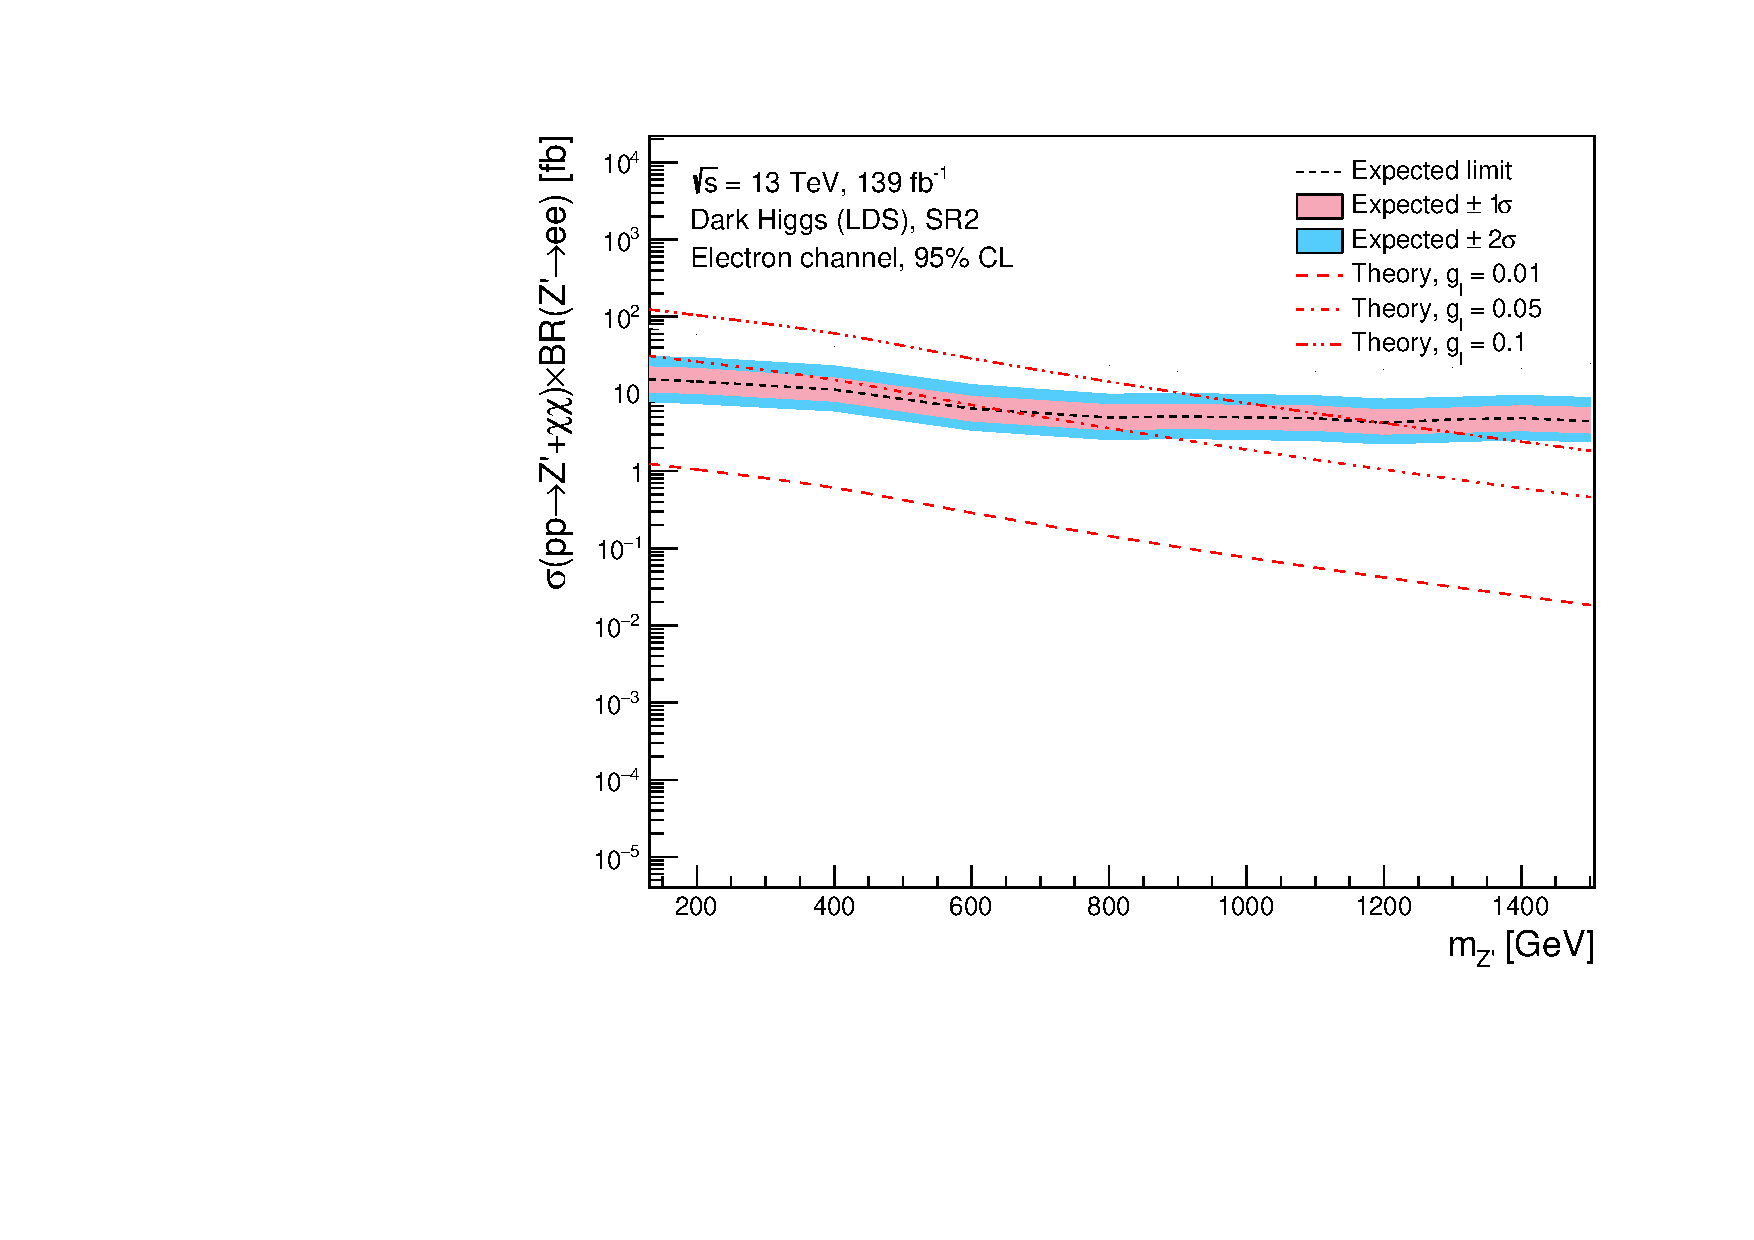
\includegraphics[width=1\textwidth]{Limits/Model_independent/100-150/DH_LDS/mass_exclusion_ee.pdf}
   \end{subfigure}
   \hfill
   \begin{subfigure}[b]{0.49\textwidth}
      \centering
      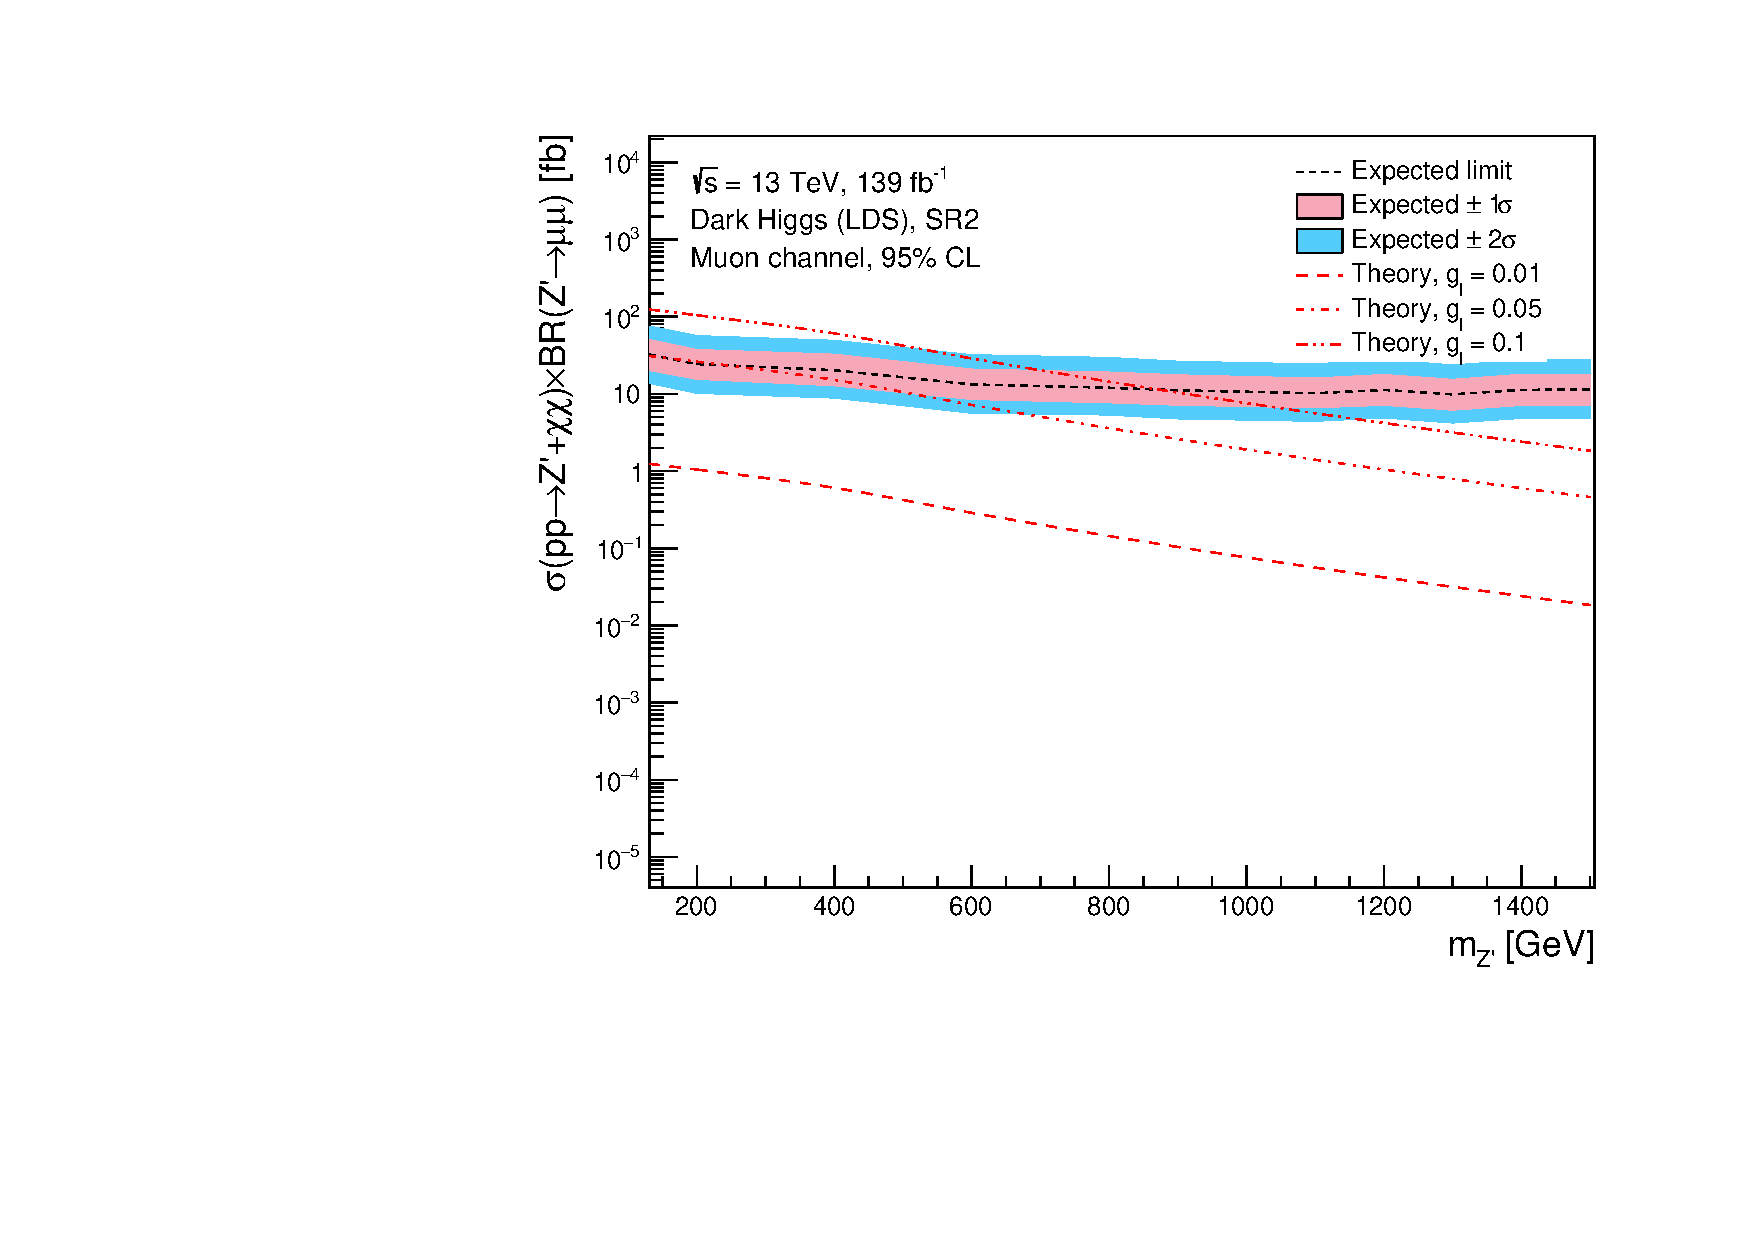
\includegraphics[width=1\textwidth]{Limits/Model_independent/100-150/DH_LDS/mass_exclusion_uu.pdf}
   \end{subfigure}
   \hfill
	\begin{subfigure}[b]{0.49\textwidth}
      \centering
      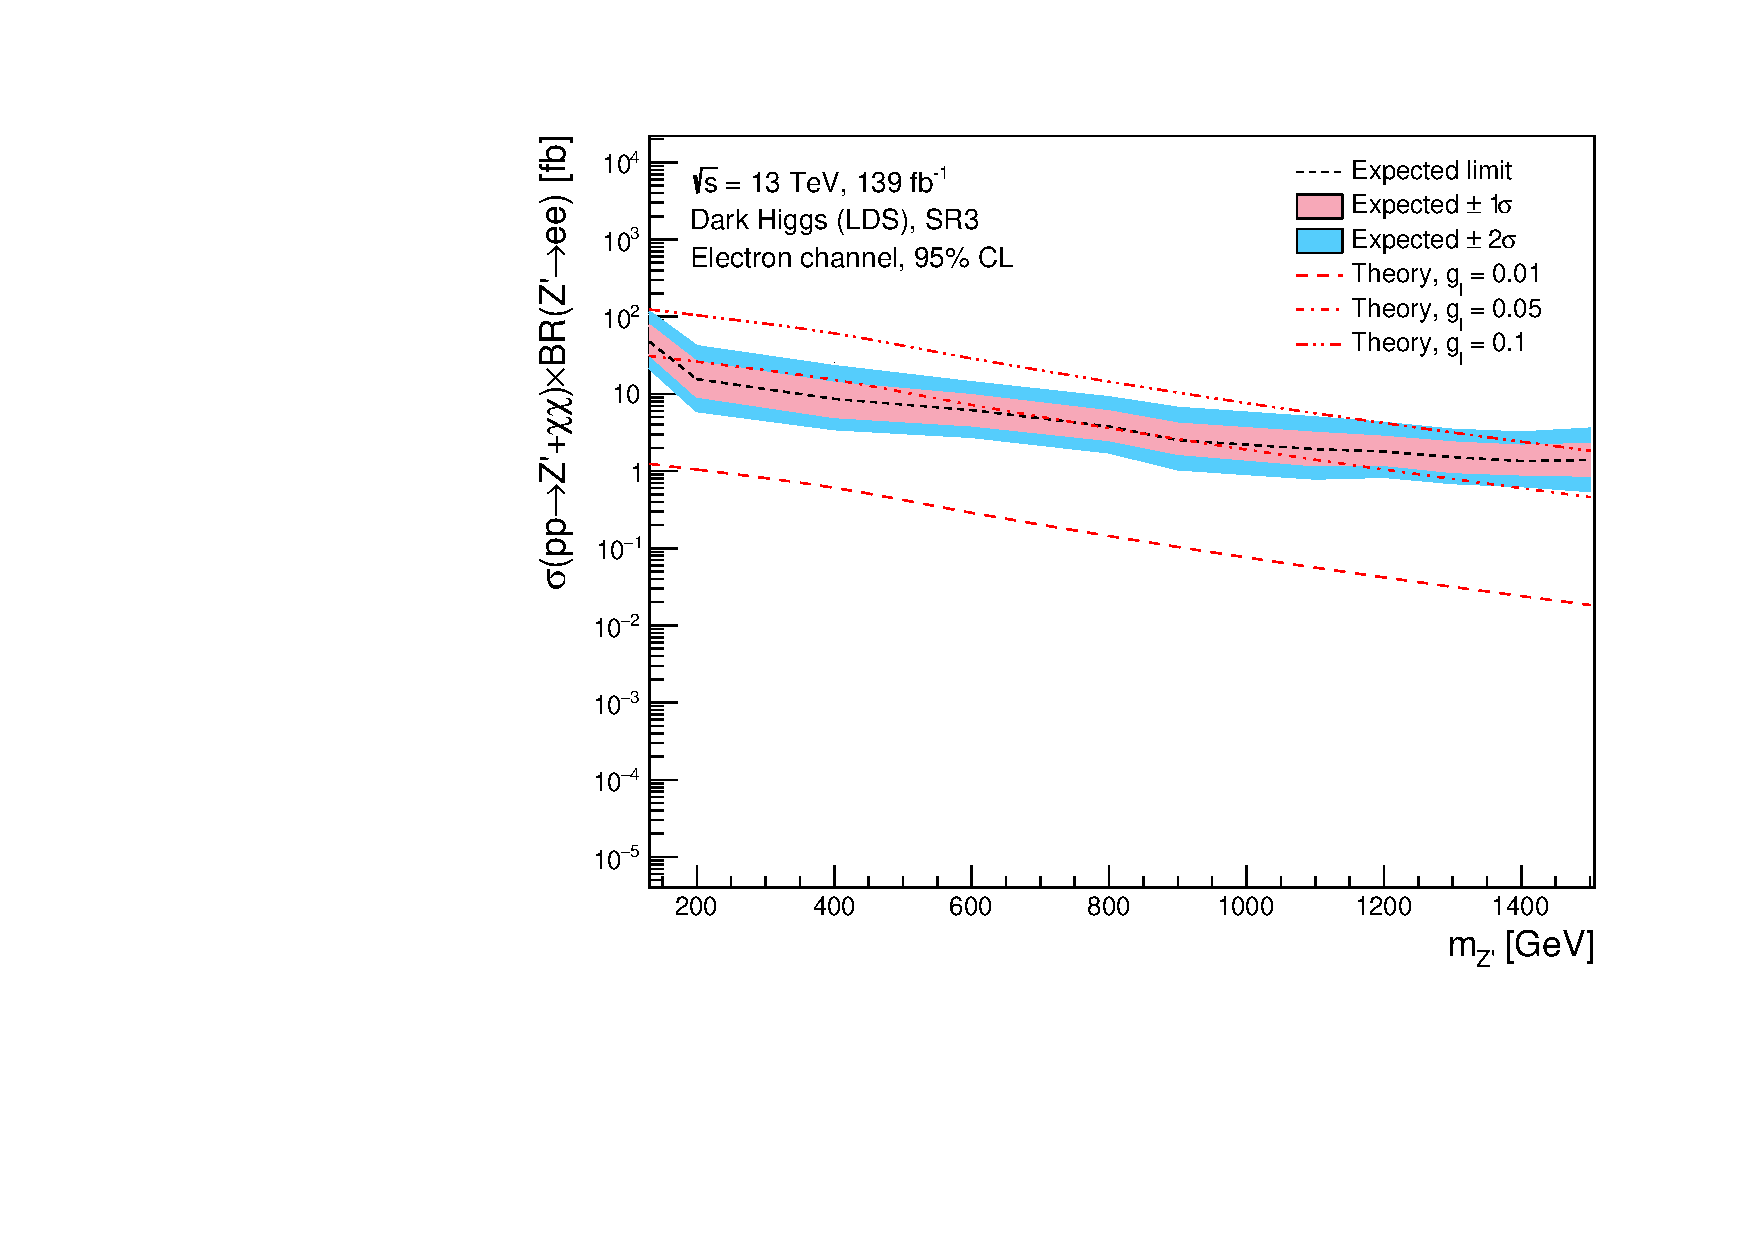
\includegraphics[width=1\textwidth]{Limits/Model_independent/150/DH_LDS/mass_exclusion_ee.pdf}
   \end{subfigure}
   \hfill
   \begin{subfigure}[b]{0.49\textwidth}
      \centering
      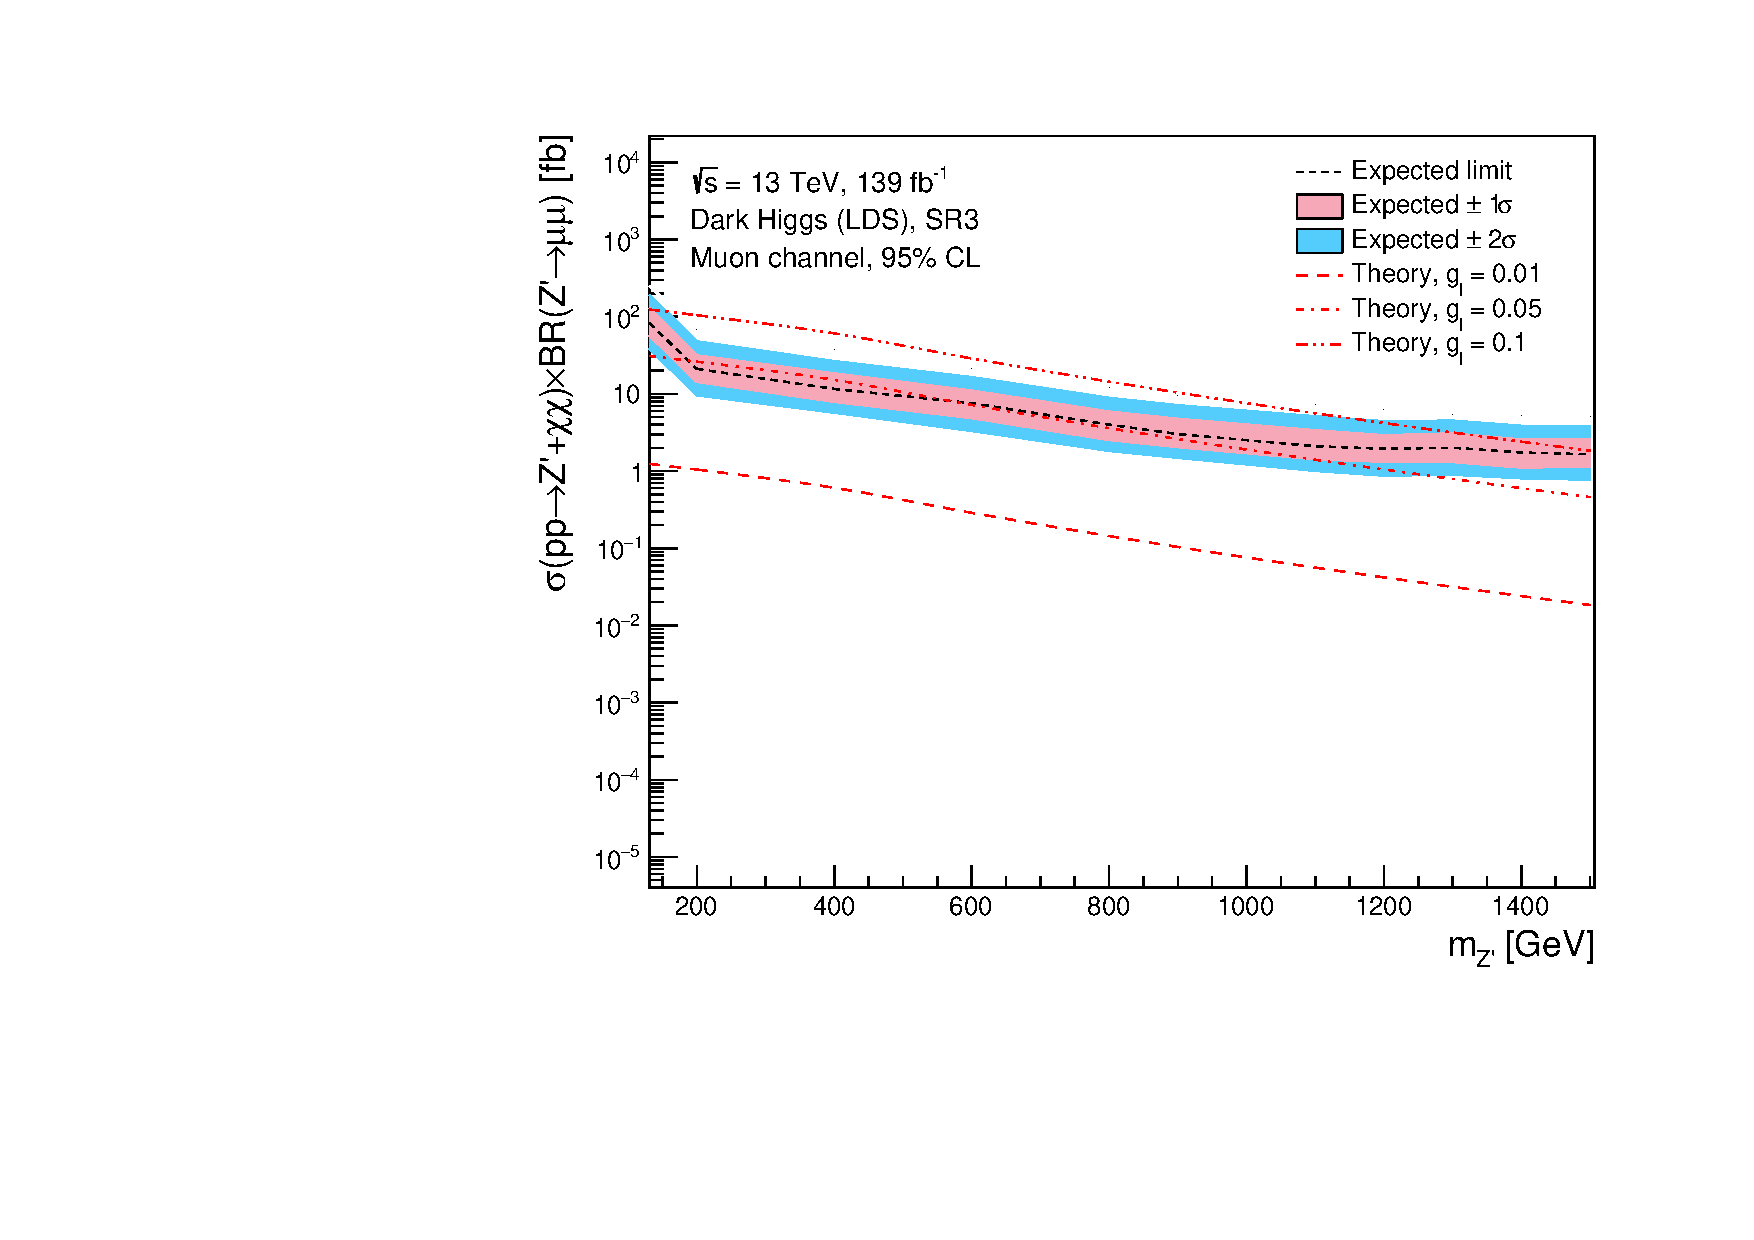
\includegraphics[width=1\textwidth]{Limits/Model_independent/150/DH_LDS/mass_exclusion_uu.pdf}
   \end{subfigure}
   \caption{Mass exclusiion limits results for DH LDS model on $ee$ and $\mu\mu$ channel in all SRs}\label{fig:DH_LDS_me_SRS}
\end{figure}

\begin{figure}[!ht]
	\centering
	\begin{subfigure}[b]{0.49\textwidth}
      \centering
      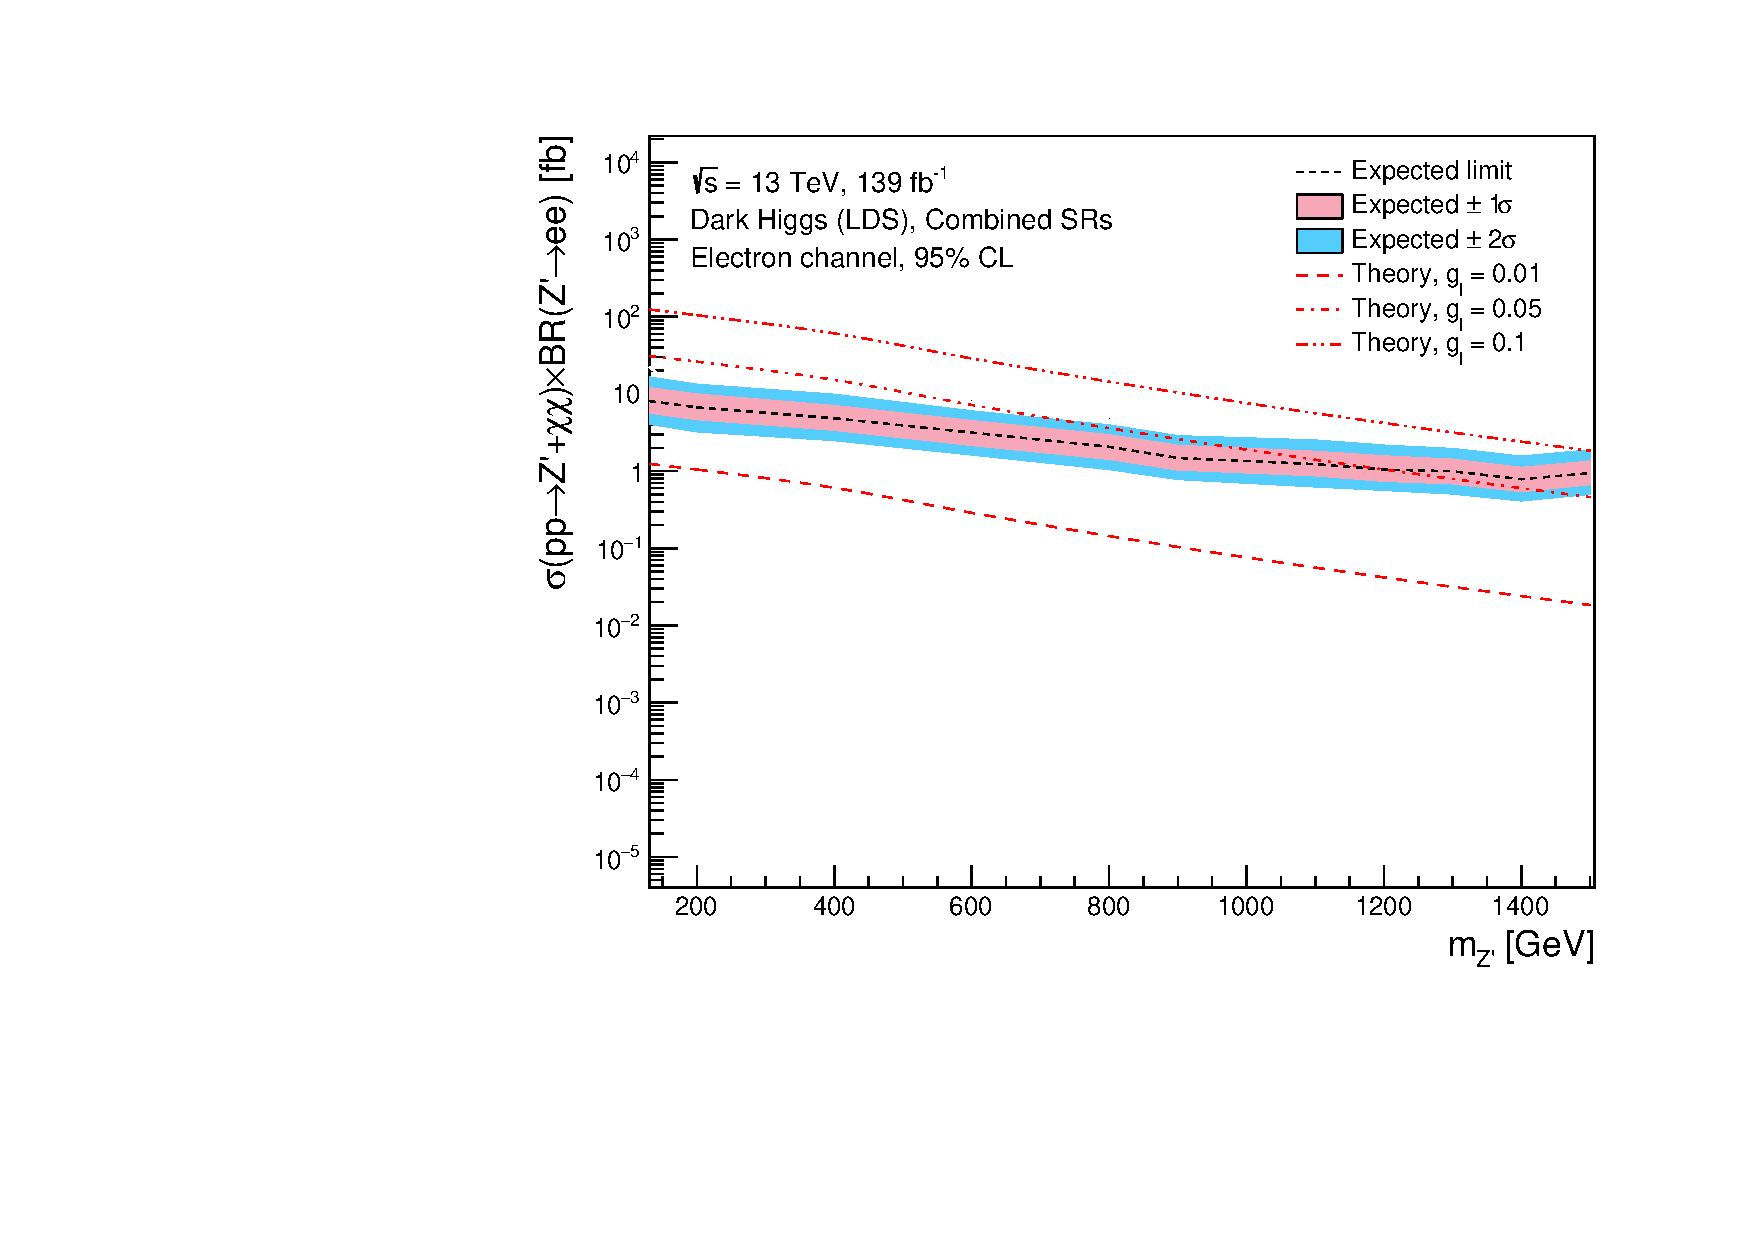
\includegraphics[width=1\textwidth]{Limits/Model_independent/DH_LDS/mass_exclusion_ee.pdf}
   \end{subfigure}
   \hfill
   \begin{subfigure}[b]{0.49\textwidth}
      \centering
      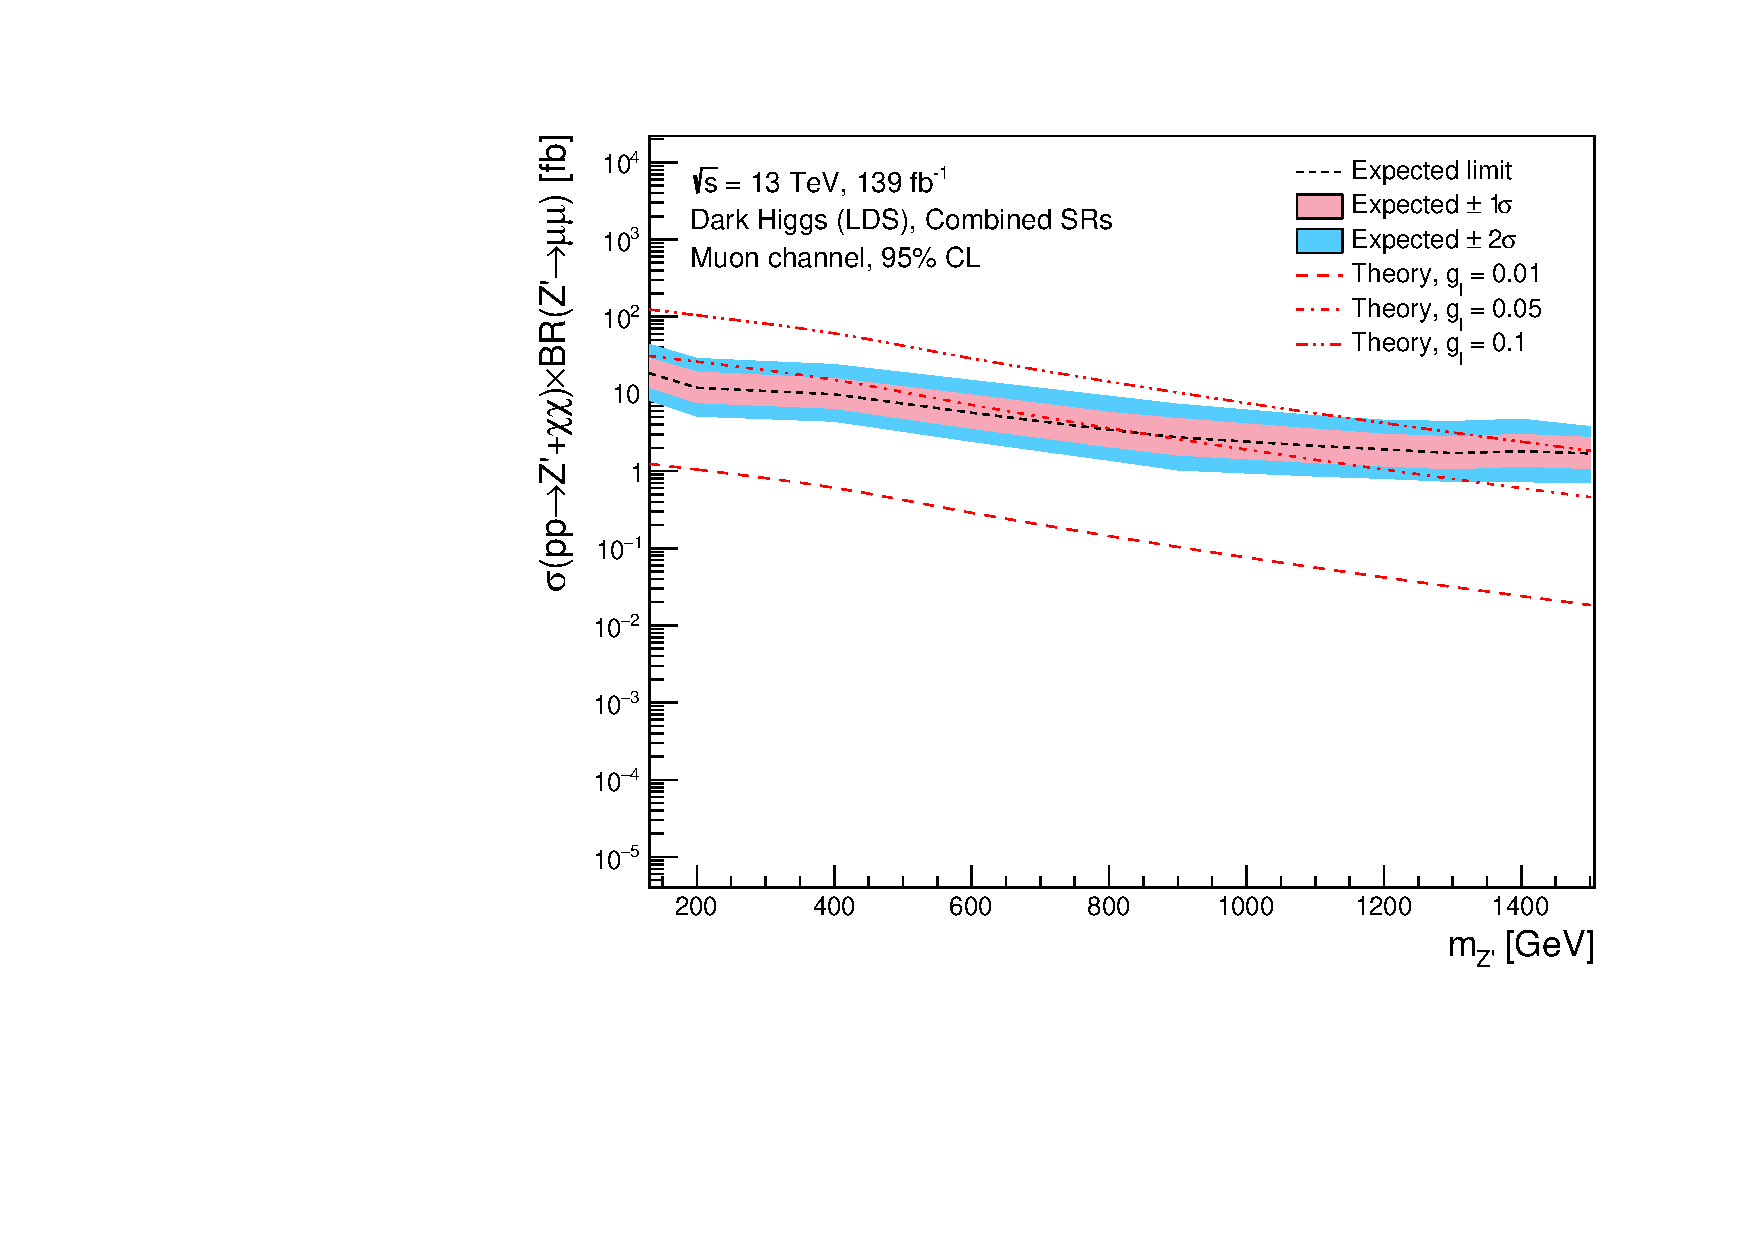
\includegraphics[width=1\textwidth]{Limits/Model_independent/DH_LDS/mass_exclusion_uu.pdf}
   \end{subfigure}
   \caption{Mass exclusiion limits results for DH LDS model on $ee$ and $\mu\mu$ channel in combined SRs}\label{fig:DH_LDS_me_comb}
\end{figure}

\clearpage

\section{Light Vector Heavy Dark Sector}
\begin{figure}[!ht]
	\centering
	\begin{subfigure}[b]{0.49\textwidth}
      \centering
      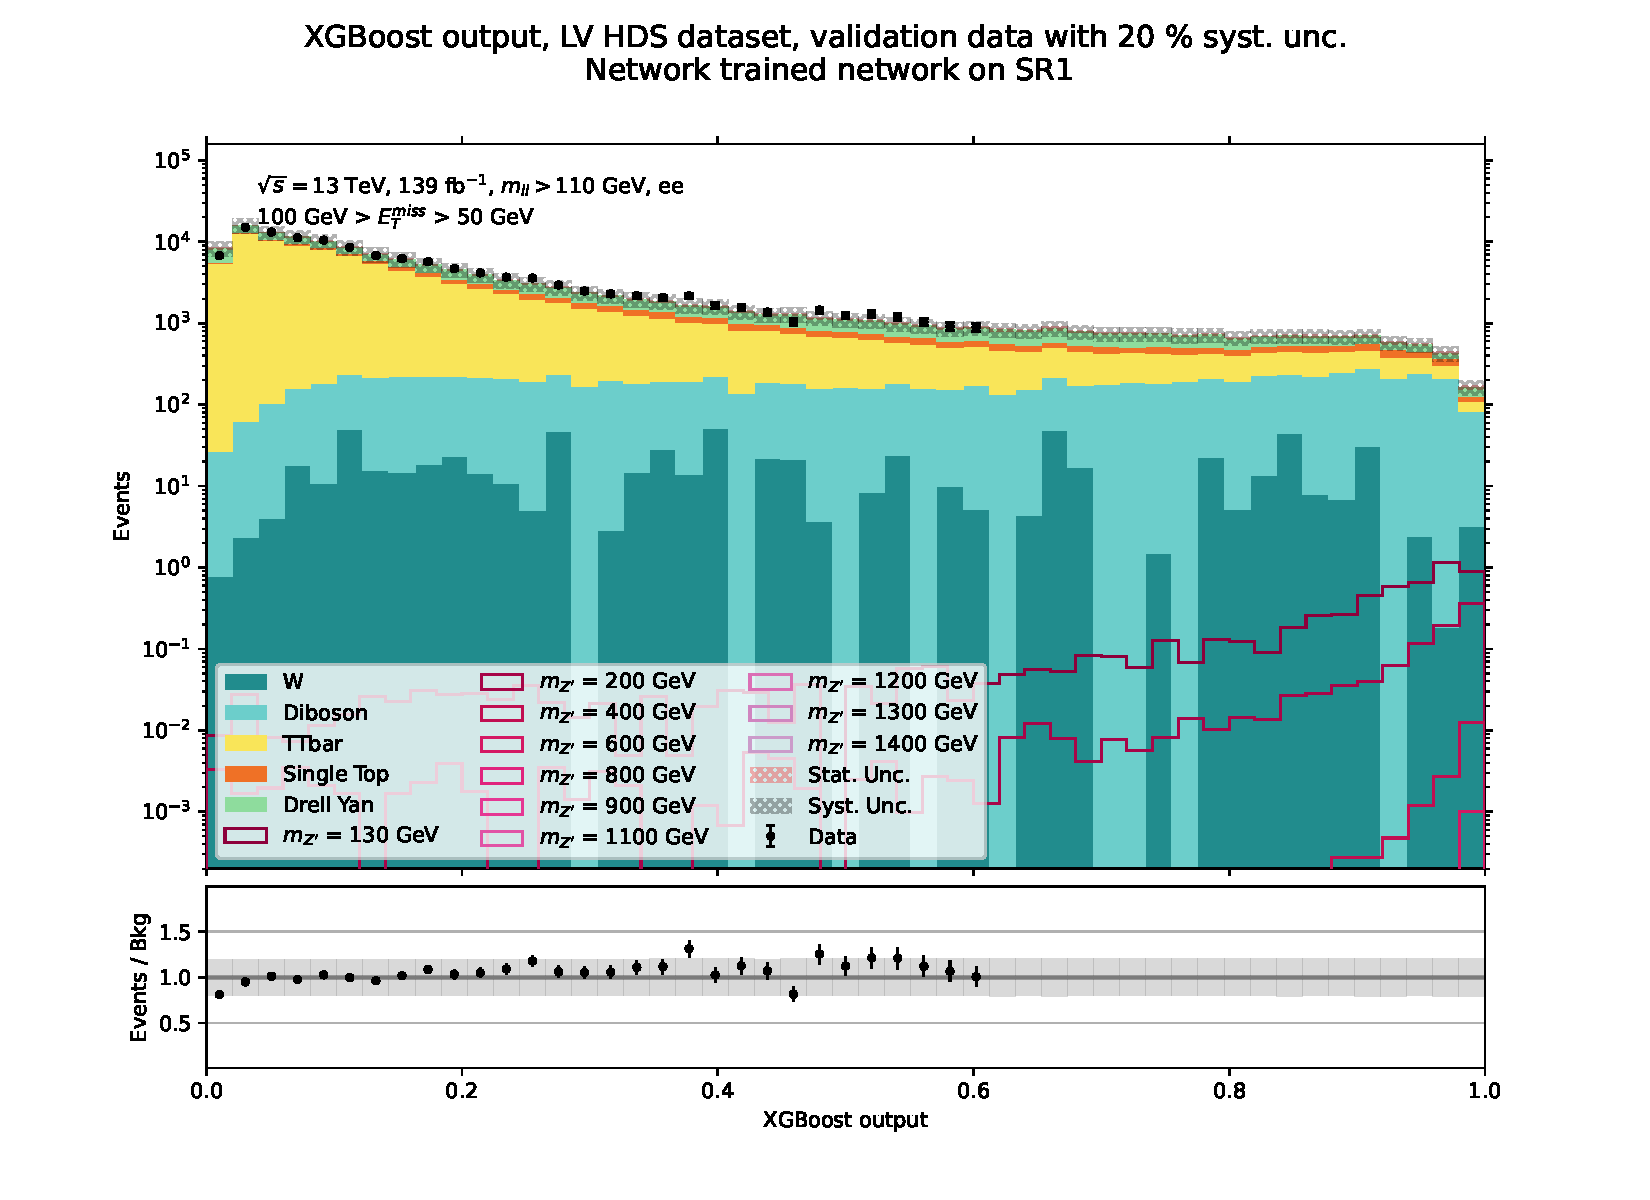
\includegraphics[width=1\textwidth]{XGBoost/Model_independent/50-100/LV_HDS/VAL_ee.pdf}
   \end{subfigure}
   \hfill
   \begin{subfigure}[b]{0.49\textwidth}
      \centering
      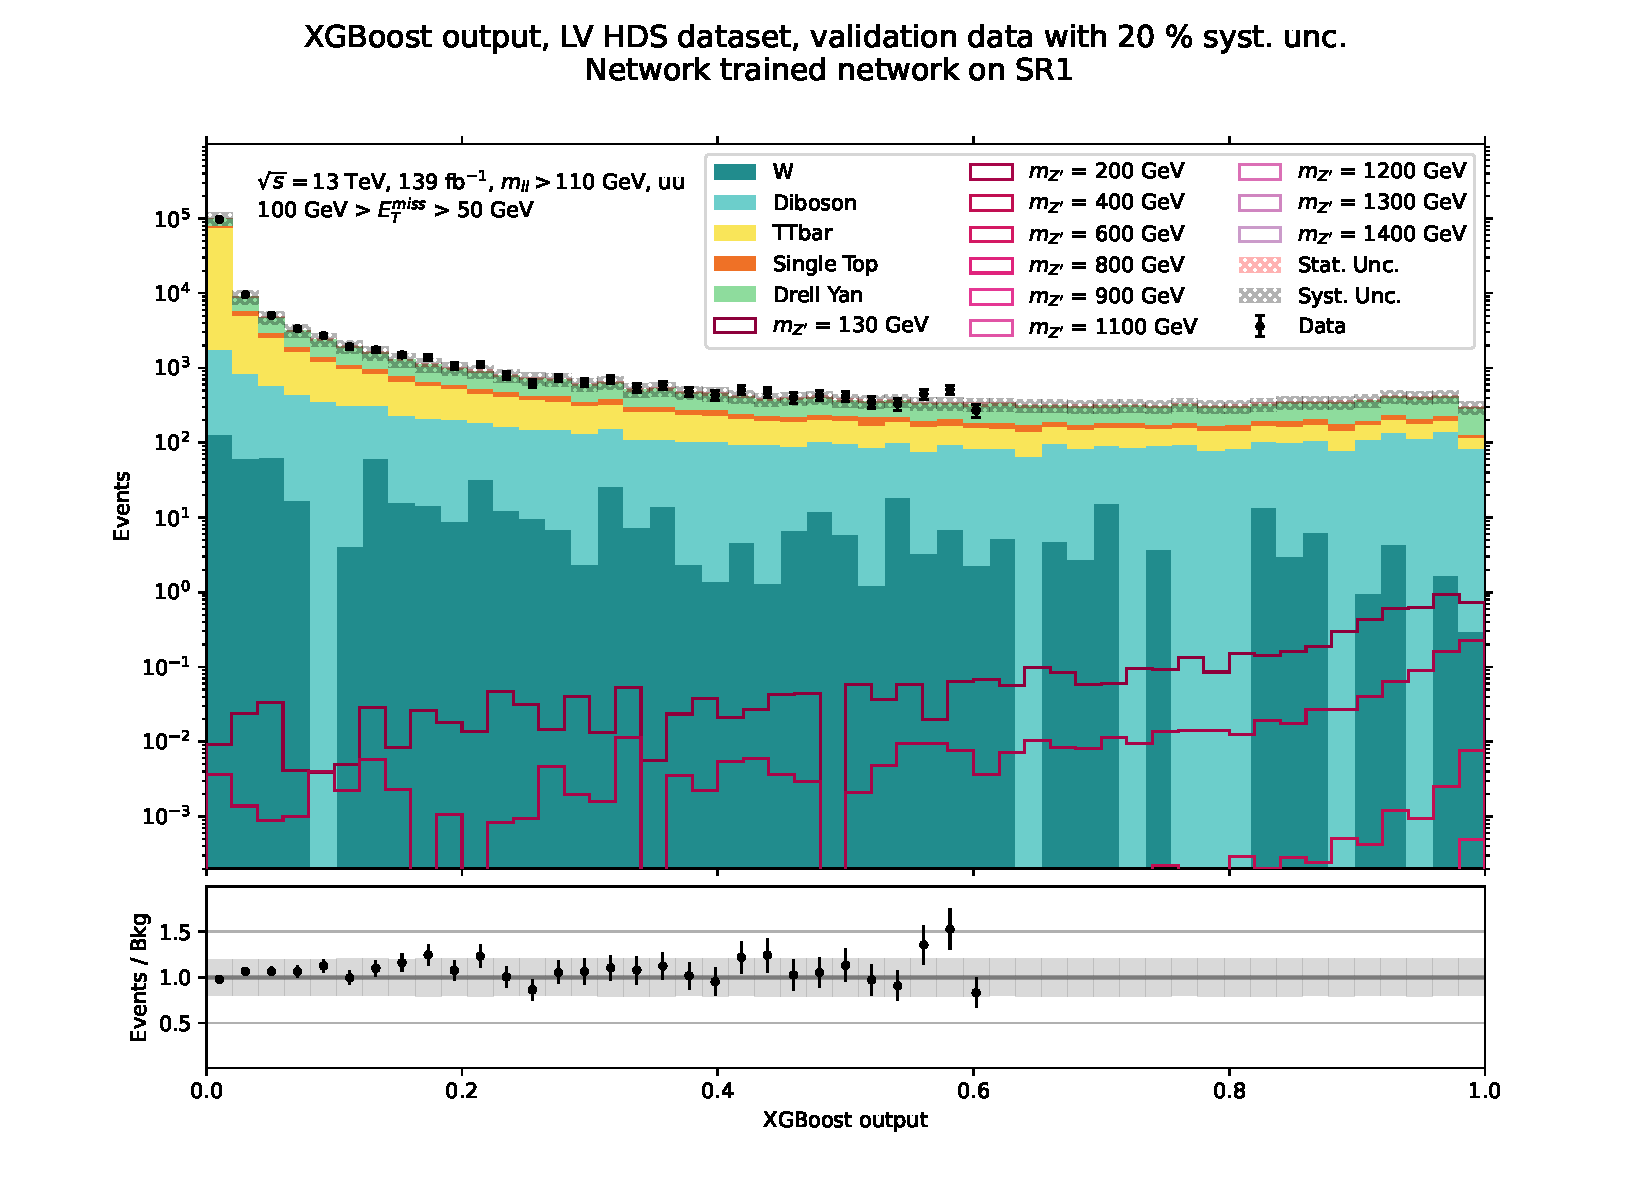
\includegraphics[width=1\textwidth]{XGBoost/Model_independent/50-100/LV_HDS/VAL_uu.pdf}
   \end{subfigure}
   \hfill
   \begin{subfigure}[b]{0.49\textwidth}
      \centering
      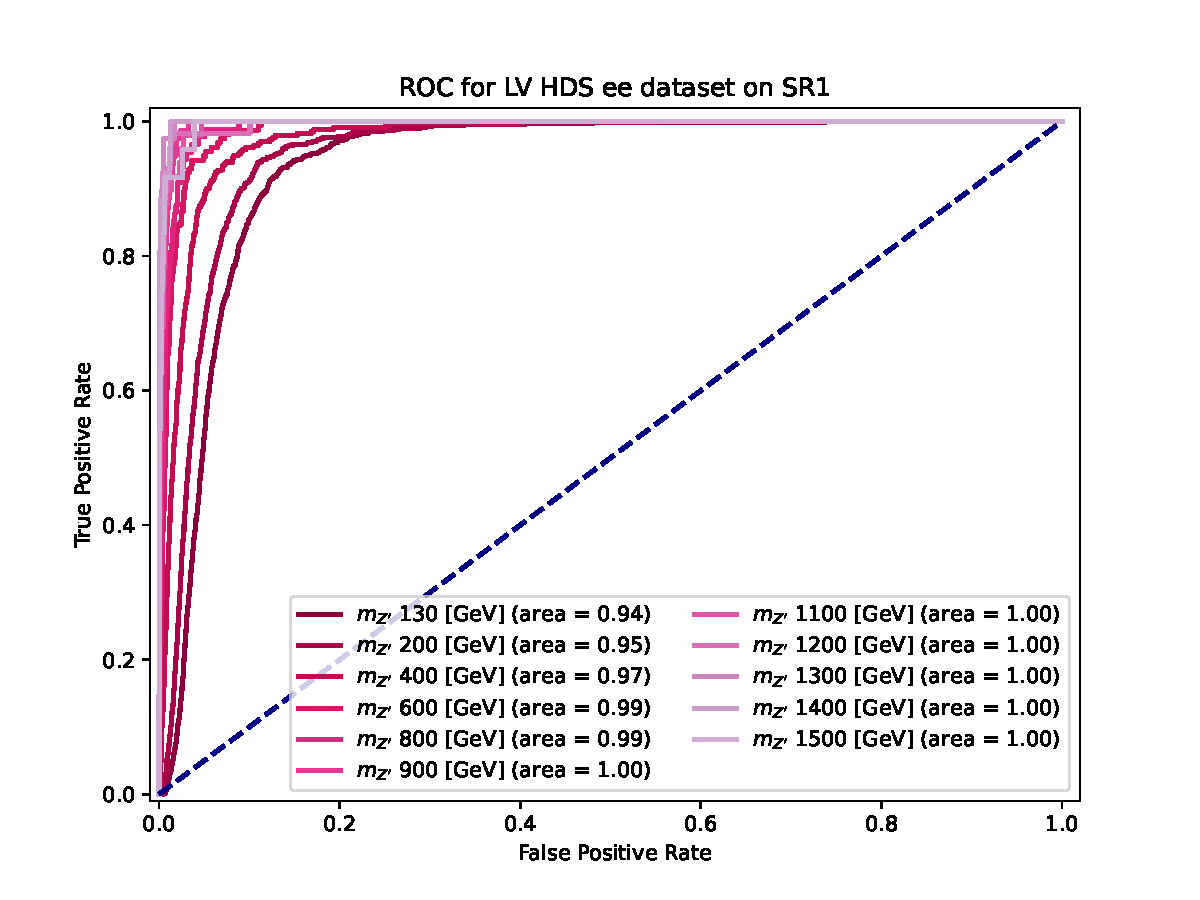
\includegraphics[width=1\textwidth]{XGBoost/Model_independent/50-100/LV_HDS/ROC_ee.pdf}
   \end{subfigure}
   \hfill
   \begin{subfigure}[b]{0.49\textwidth}
      \centering
      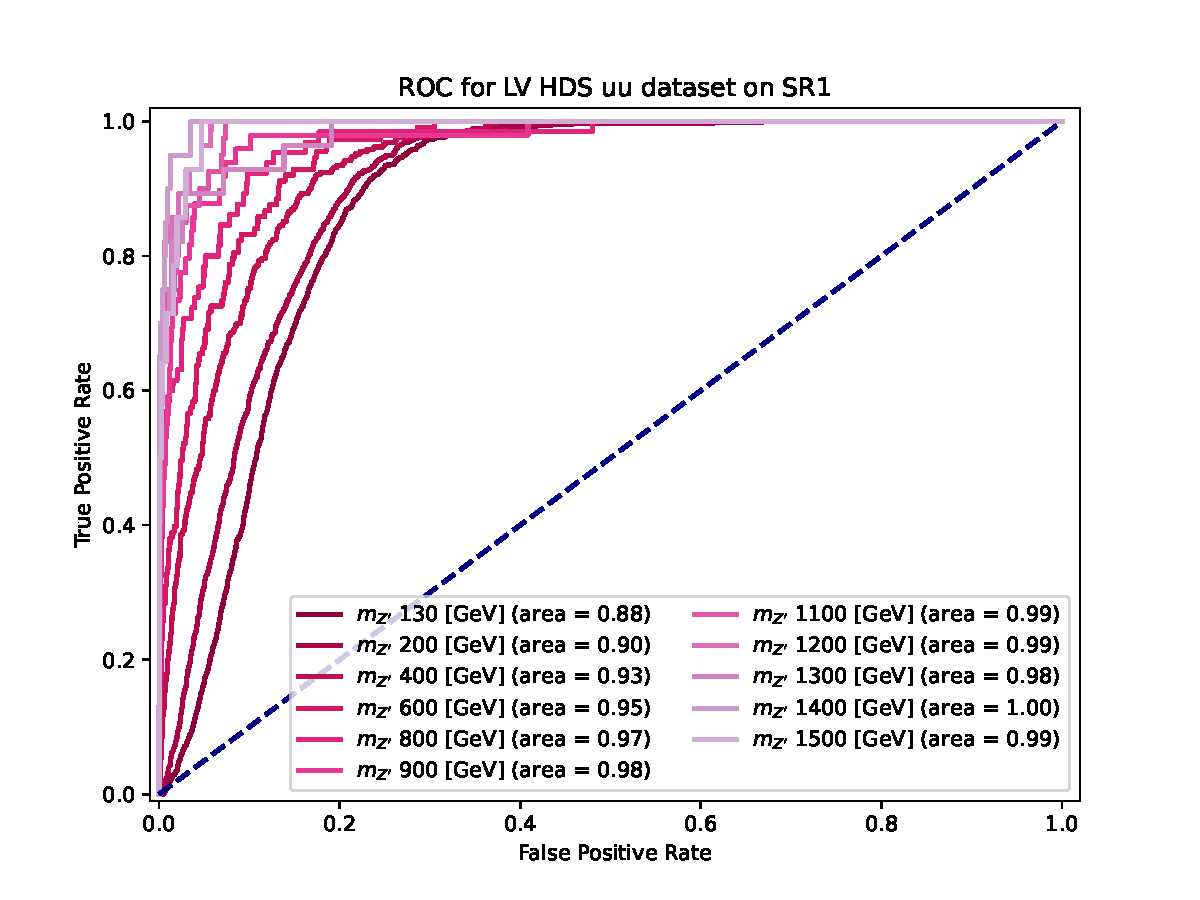
\includegraphics[width=1\textwidth]{XGBoost/Model_independent/50-100/LV_HDS/ROC_uu.pdf}
   \end{subfigure}
   \hfill
	\begin{subfigure}[b]{0.49\textwidth}
      \centering
      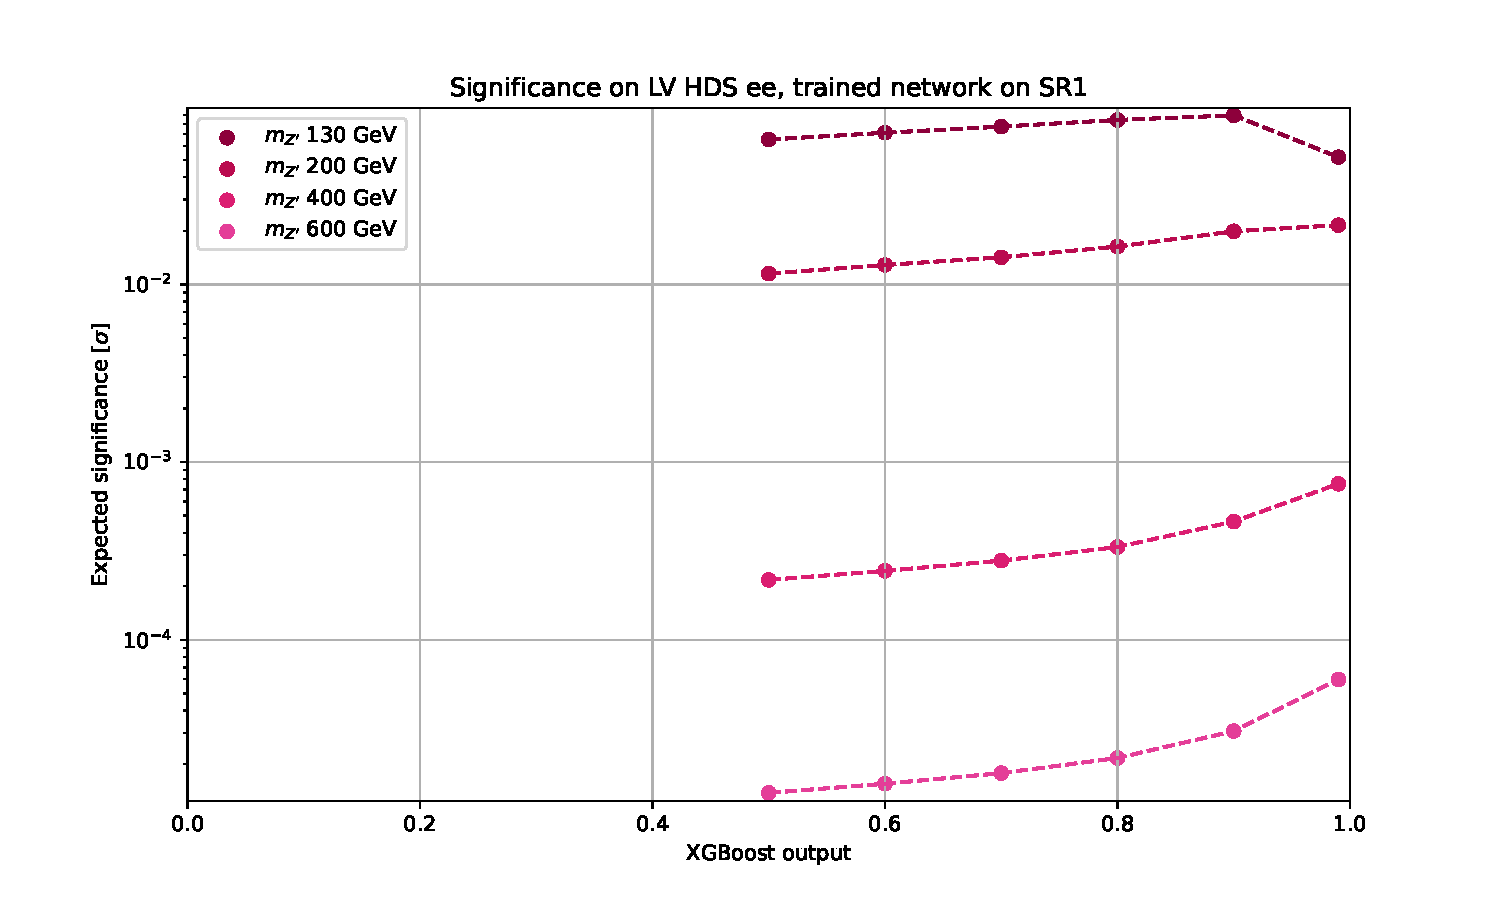
\includegraphics[width=1\textwidth]{XGBoost/Model_independent/50-100/LV_HDS/EXP_SIG_ee.pdf}
   \end{subfigure}
   \hfill
   \begin{subfigure}[b]{0.49\textwidth}
      \centering
      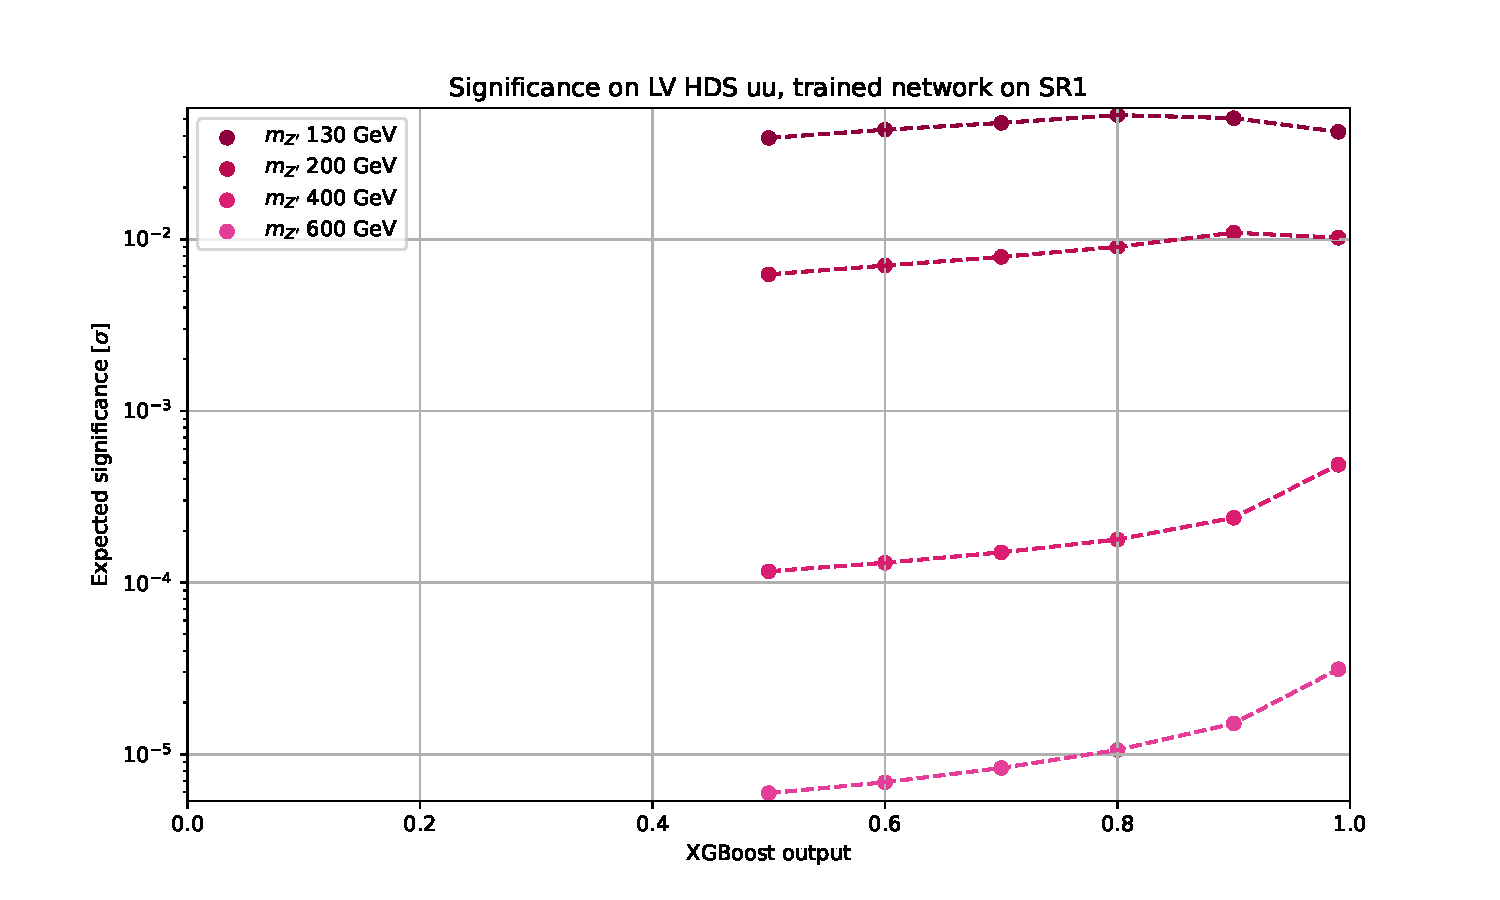
\includegraphics[width=1\textwidth]{XGBoost/Model_independent/50-100/LV_HDS/EXP_SIG_uu.pdf}
   \end{subfigure}
   \caption{XGBoost results for LV HDS model on $ee$ and $\mu\mu$ channel in SR1}\label{fig:LV_HDS_SR1}
\end{figure}

\begin{figure}[!ht]
	\centering
	\begin{subfigure}[b]{0.49\textwidth}
      \centering
      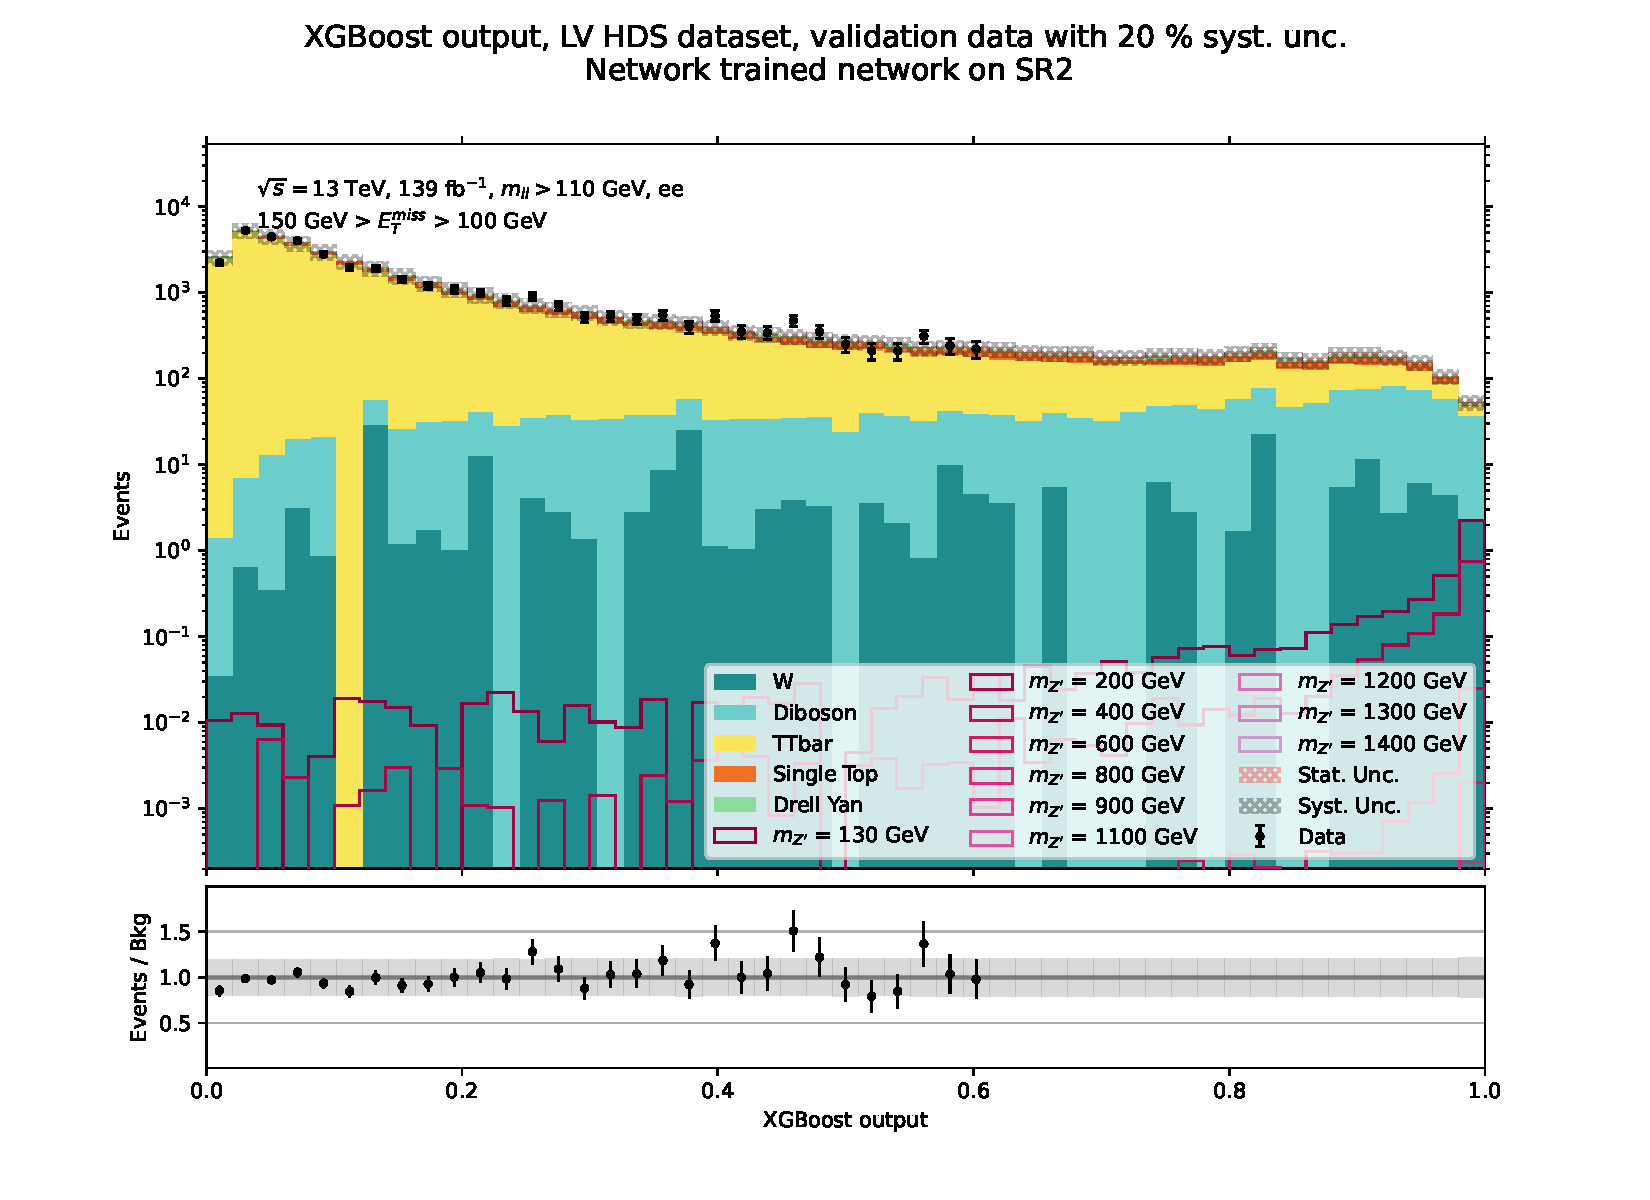
\includegraphics[width=1\textwidth]{XGBoost/Model_independent/100-150/LV_HDS/VAL_ee.pdf}
   \end{subfigure}
   \hfill
   \begin{subfigure}[b]{0.49\textwidth}
      \centering
      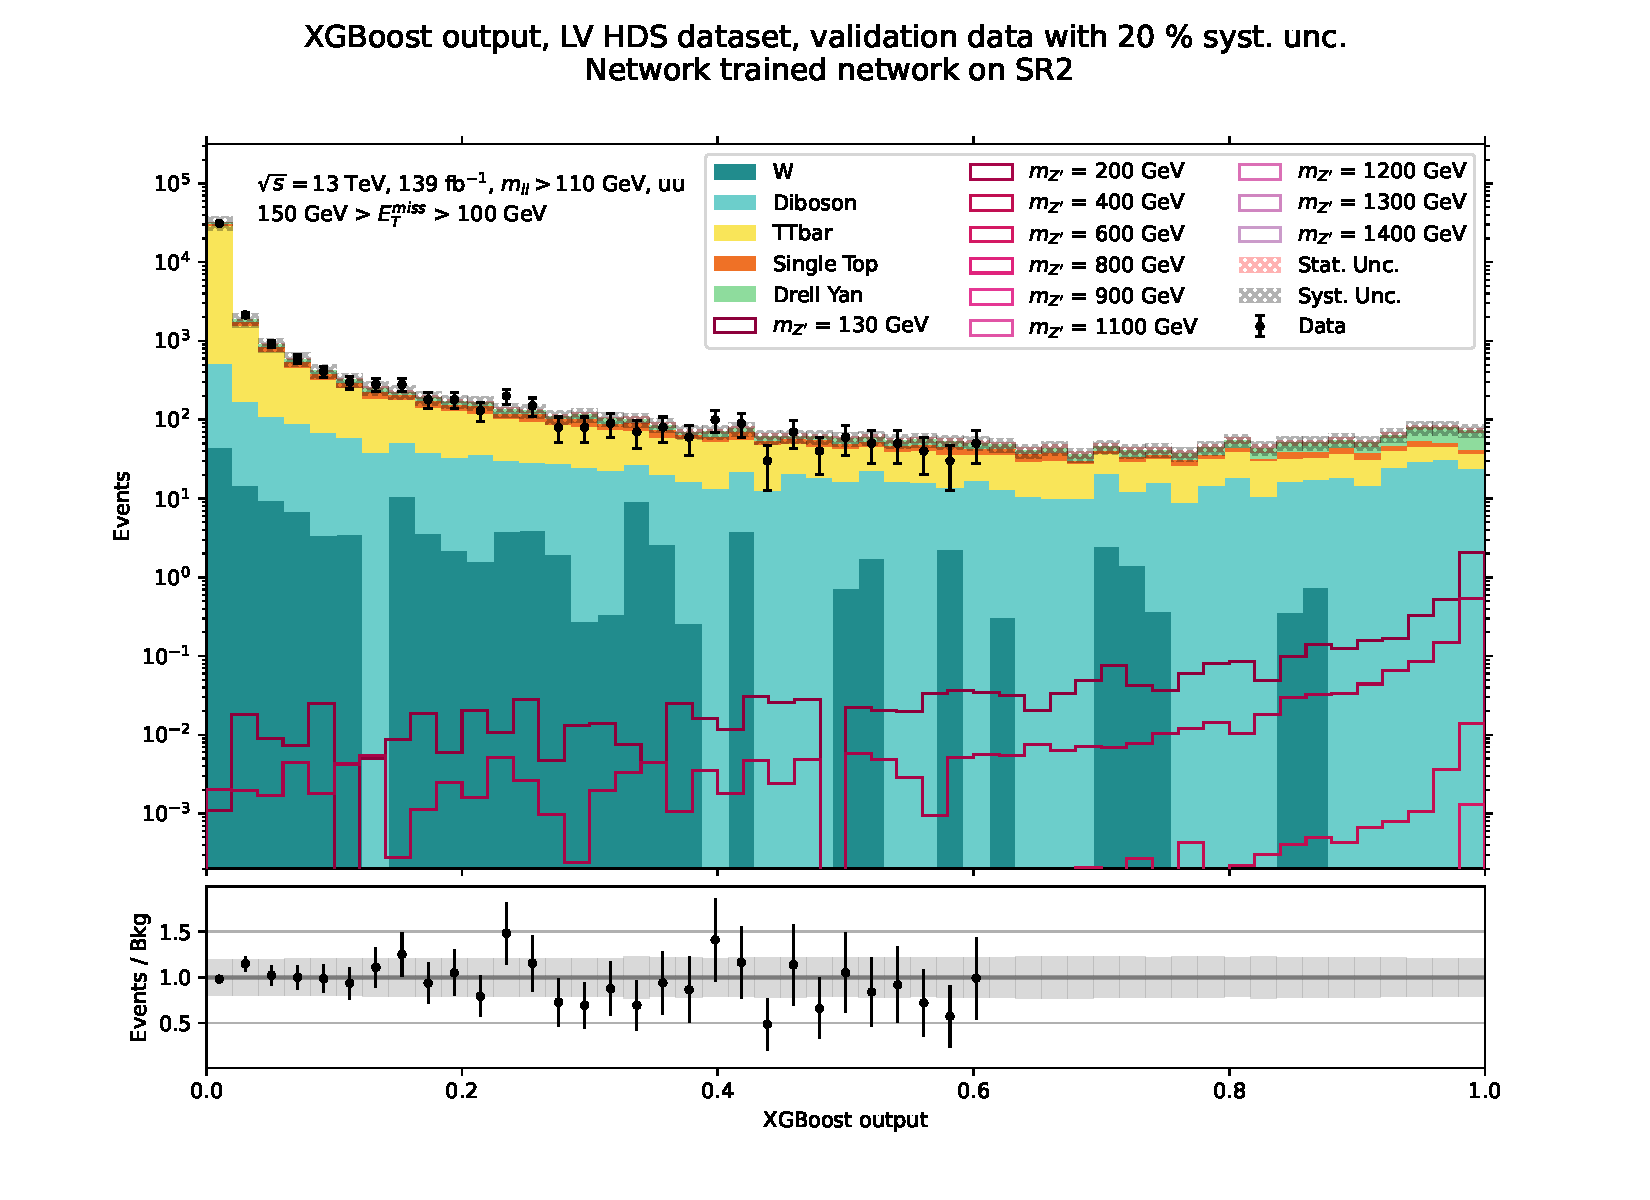
\includegraphics[width=1\textwidth]{XGBoost/Model_independent/100-150/LV_HDS/VAL_uu.pdf}
   \end{subfigure}
   \hfill
   \begin{subfigure}[b]{0.49\textwidth}
      \centering
      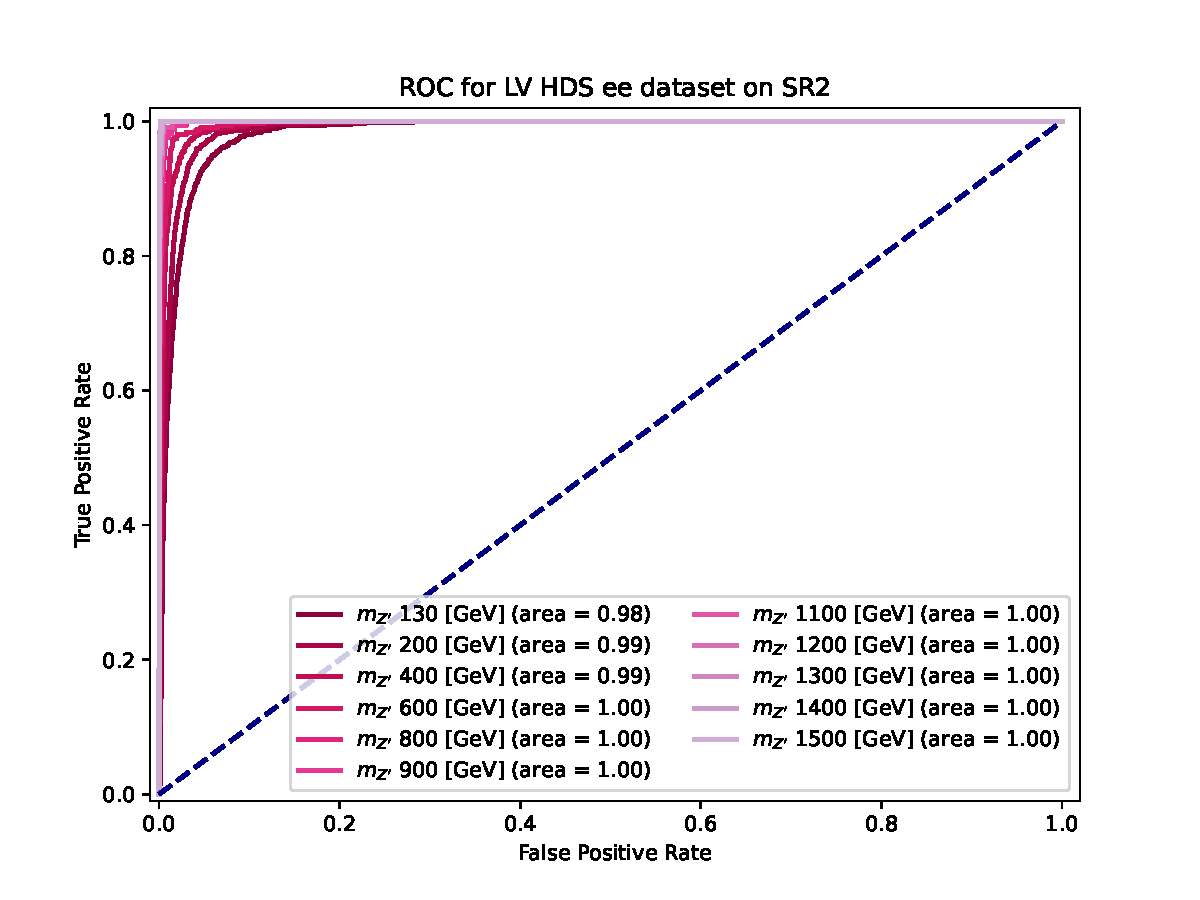
\includegraphics[width=1\textwidth]{XGBoost/Model_independent/100-150/LV_HDS/ROC_ee.pdf}
   \end{subfigure}
   \hfill
   \begin{subfigure}[b]{0.49\textwidth}
      \centering
      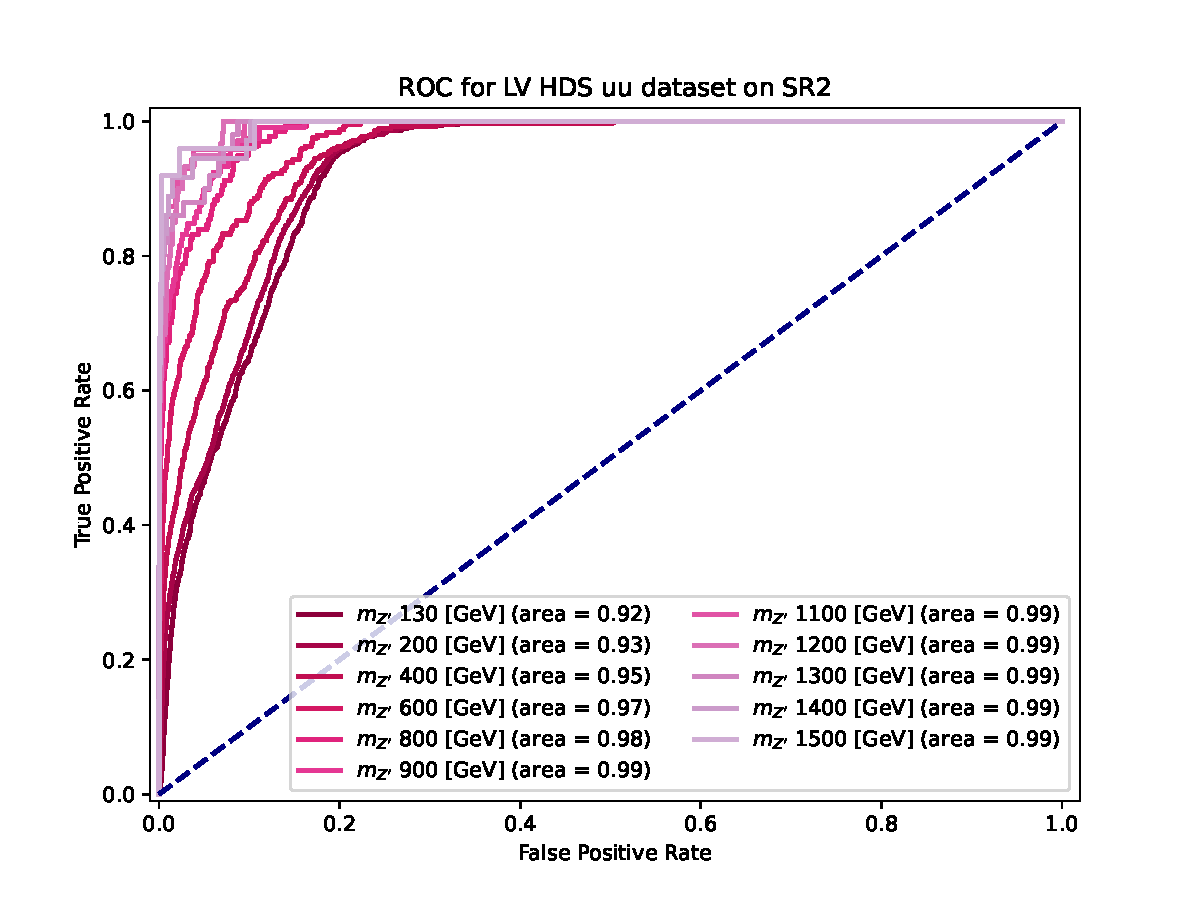
\includegraphics[width=1\textwidth]{XGBoost/Model_independent/100-150/LV_HDS/ROC_uu.pdf}
   \end{subfigure}
   \hfill
	\begin{subfigure}[b]{0.49\textwidth}
      \centering
      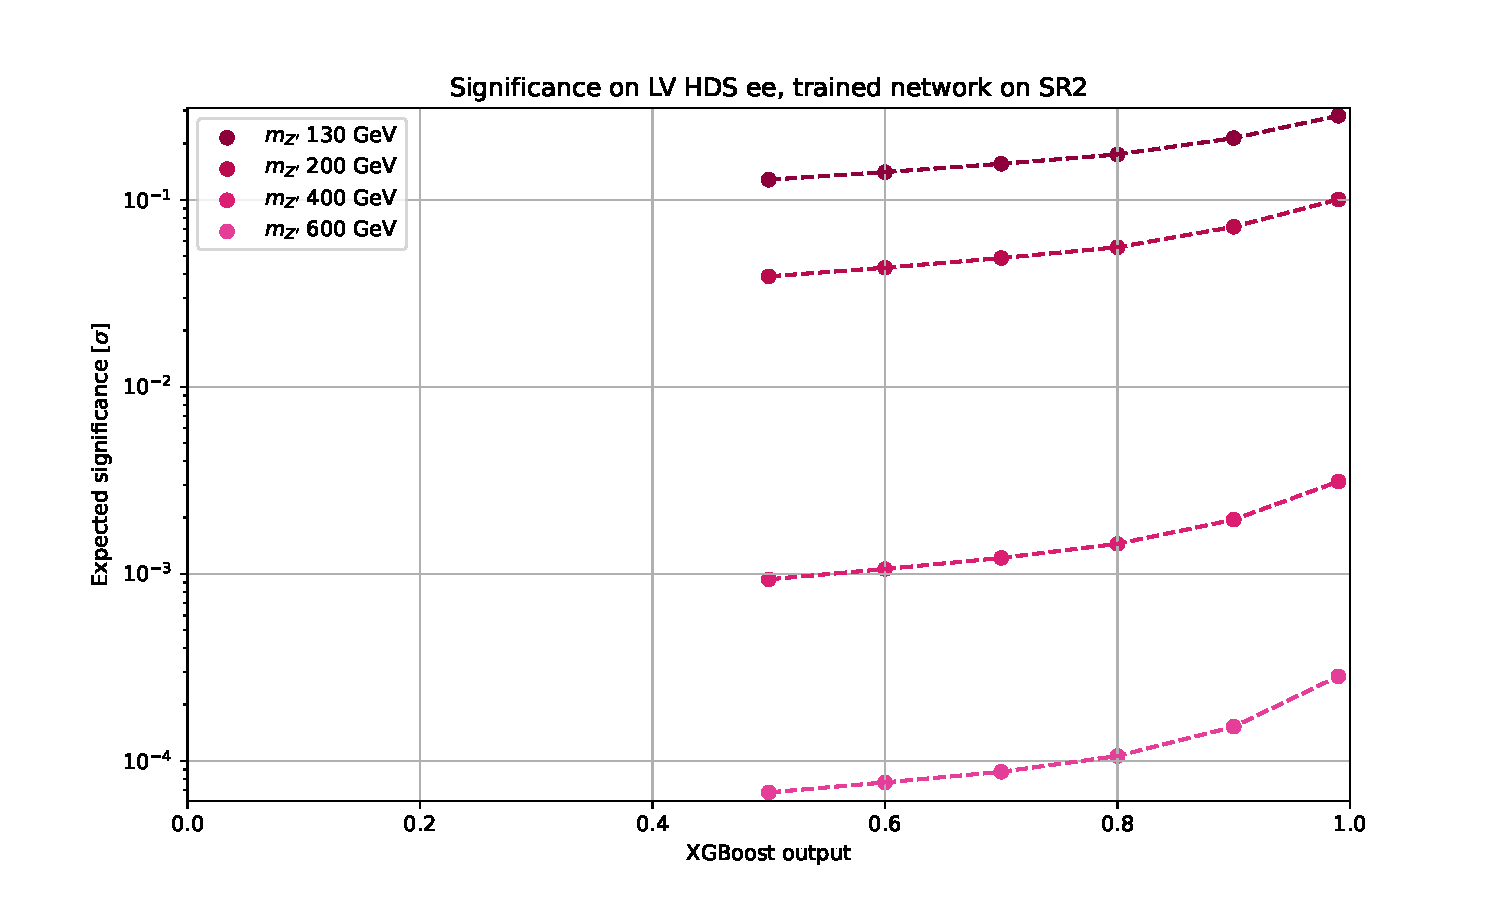
\includegraphics[width=1\textwidth]{XGBoost/Model_independent/100-150/LV_HDS/EXP_SIG_ee.pdf}
   \end{subfigure}
   \hfill
   \begin{subfigure}[b]{0.49\textwidth}
      \centering
      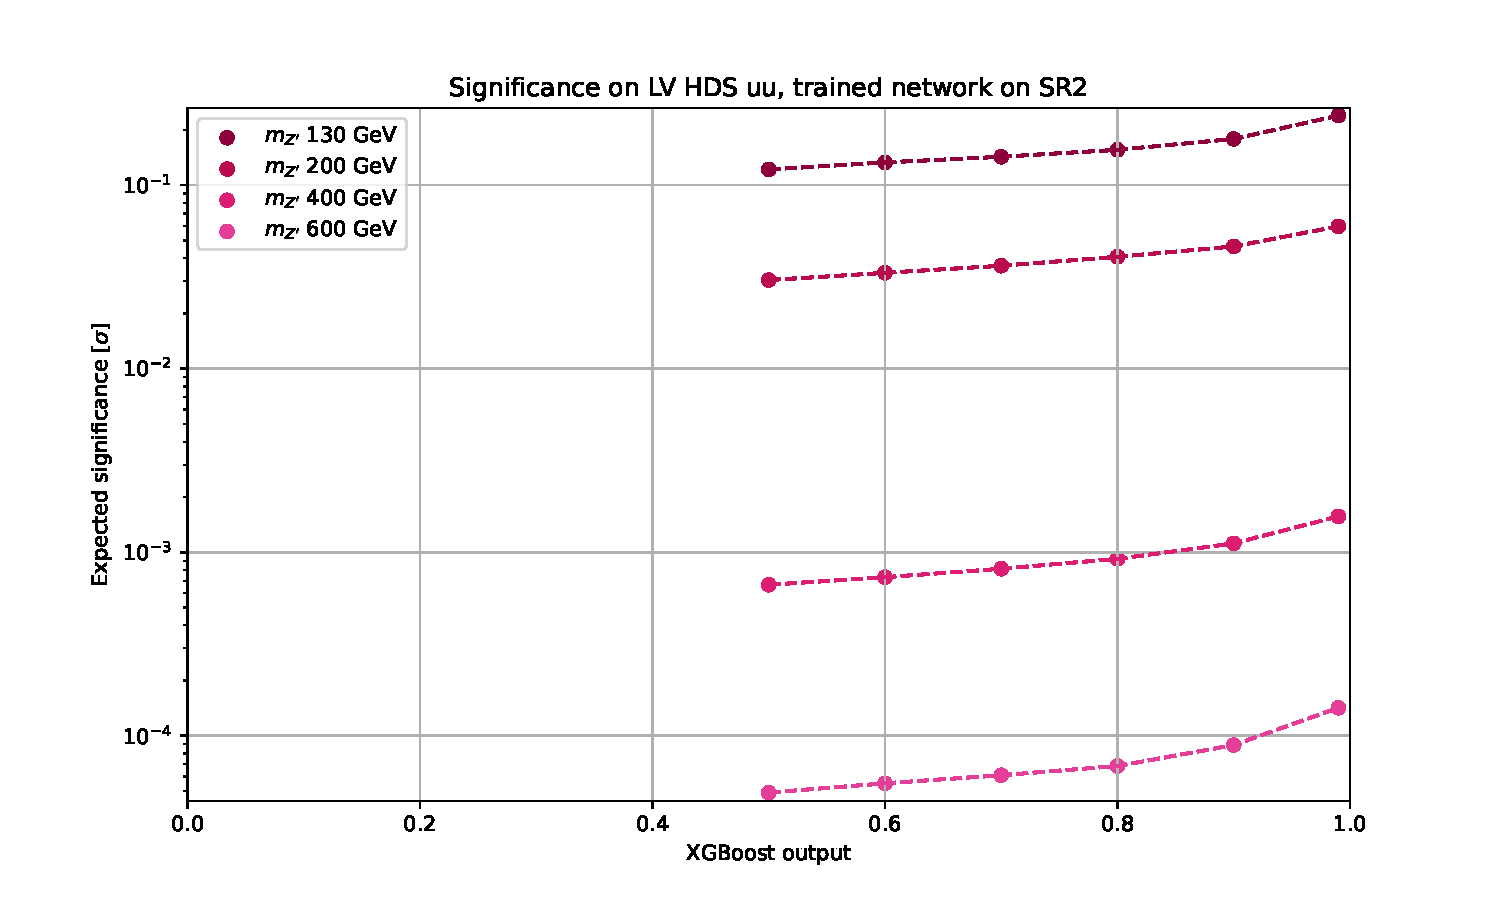
\includegraphics[width=1\textwidth]{XGBoost/Model_independent/100-150/LV_HDS/EXP_SIG_uu.pdf}
   \end{subfigure}
   \caption{XGBoost results for LV HDS model on $ee$ and $\mu\mu$ channel in SR2}\label{fig:LV_HDS_SR2}
\end{figure}

\begin{figure}[!ht]
	\centering
	\begin{subfigure}[b]{0.49\textwidth}
      \centering
      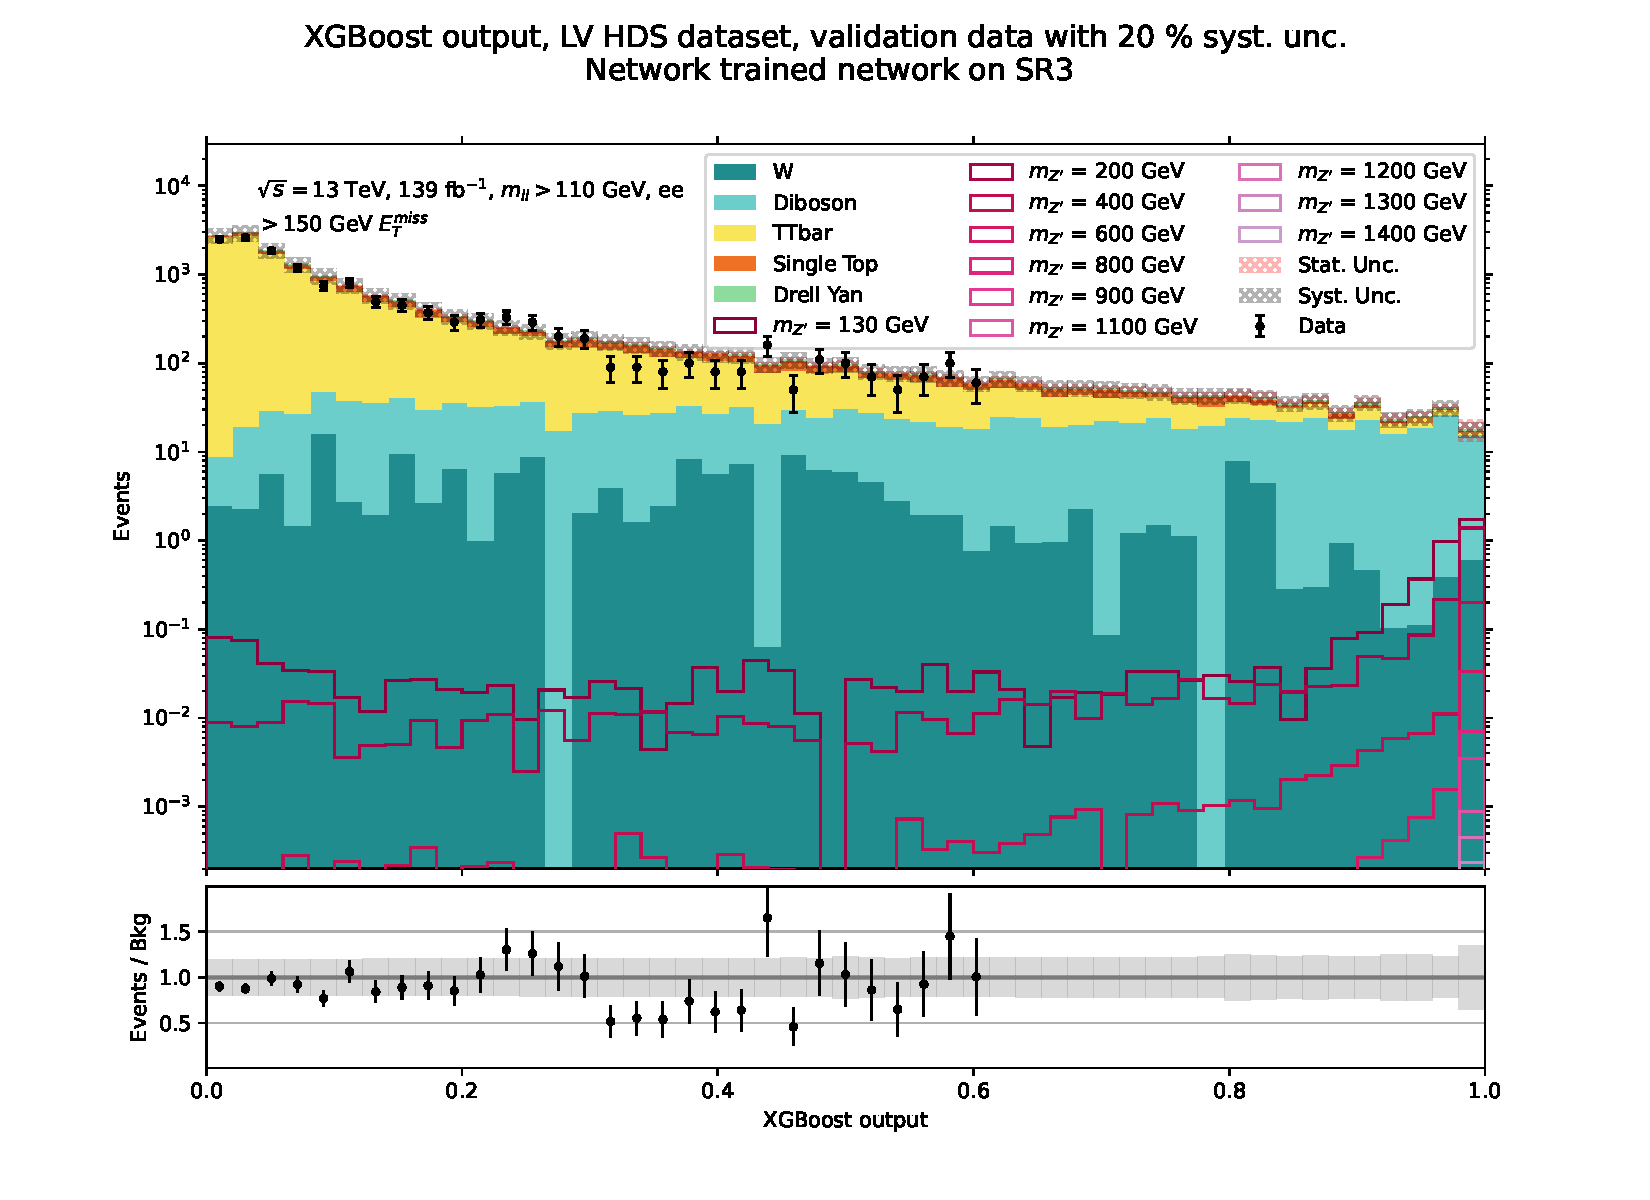
\includegraphics[width=1\textwidth]{XGBoost/Model_independent/150/LV_HDS/VAL_ee.pdf}
   \end{subfigure}
   \hfill
   \begin{subfigure}[b]{0.49\textwidth}
      \centering
      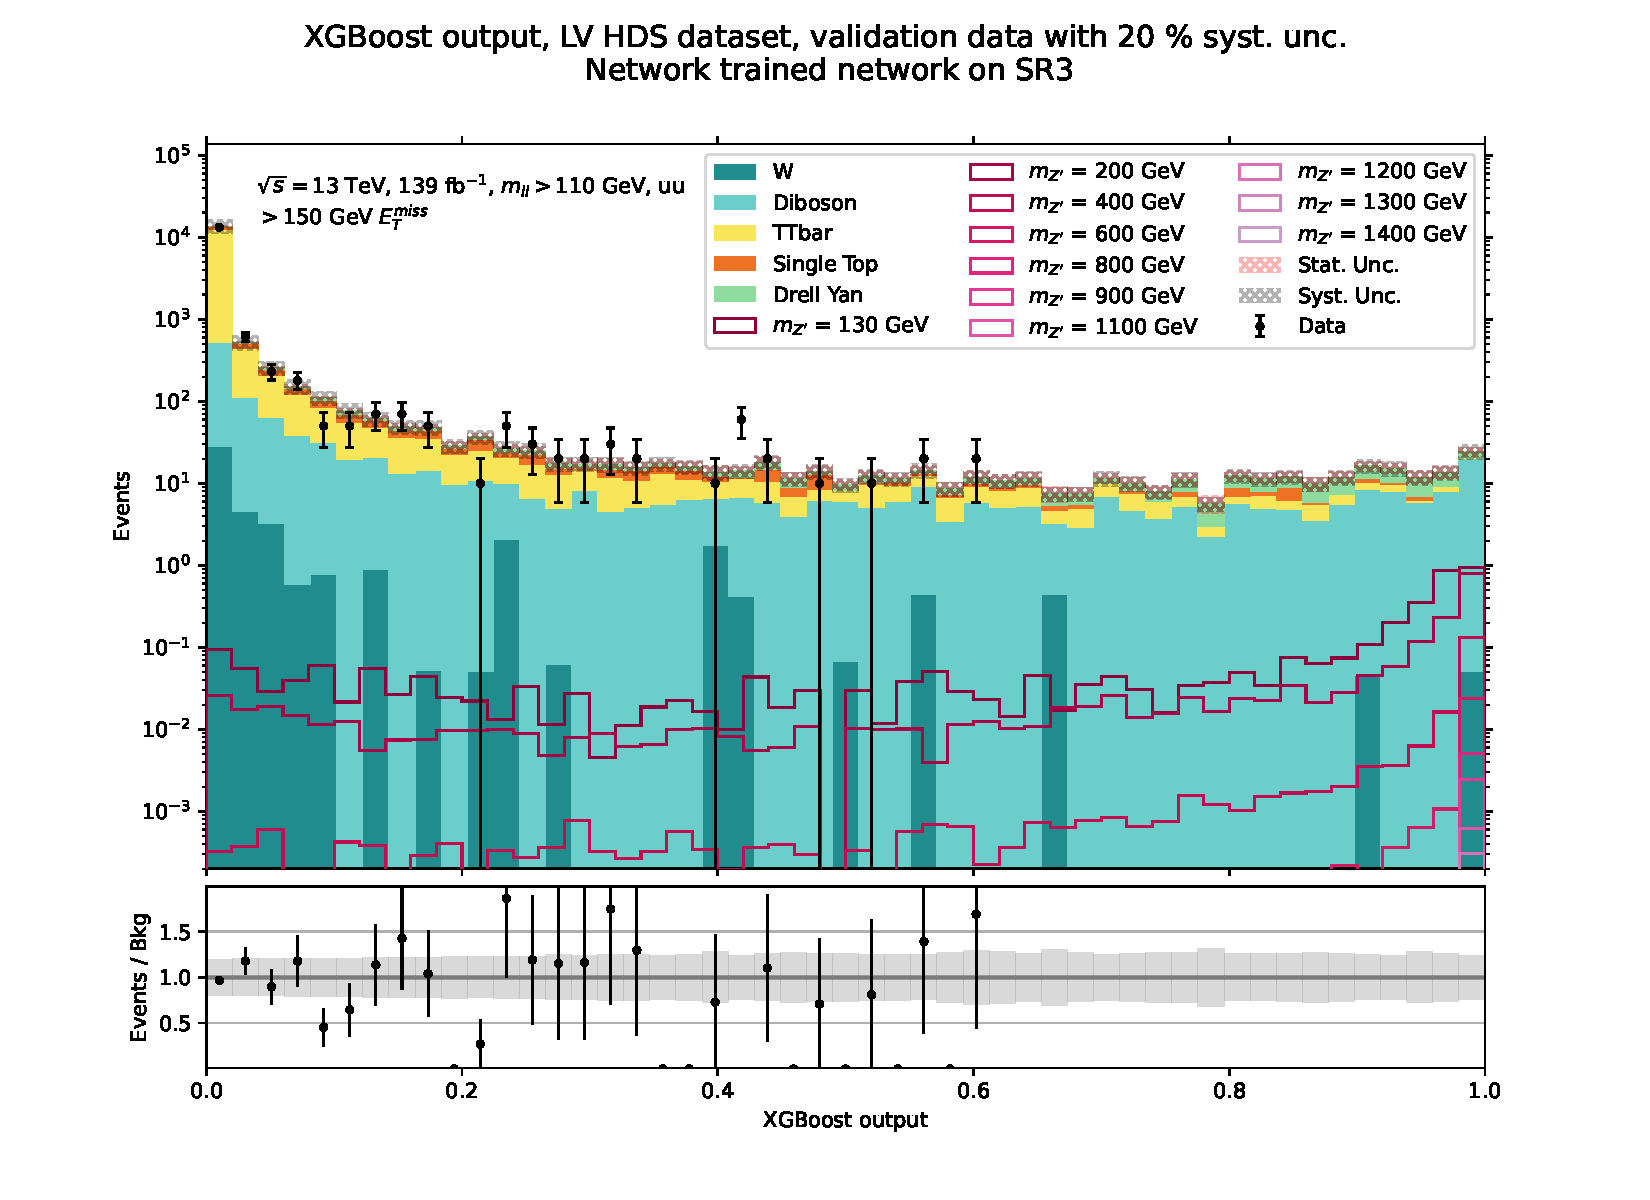
\includegraphics[width=1\textwidth]{XGBoost/Model_independent/150/LV_HDS/VAL_uu.pdf}
   \end{subfigure}
   \hfill
   \begin{subfigure}[b]{0.49\textwidth}
      \centering
      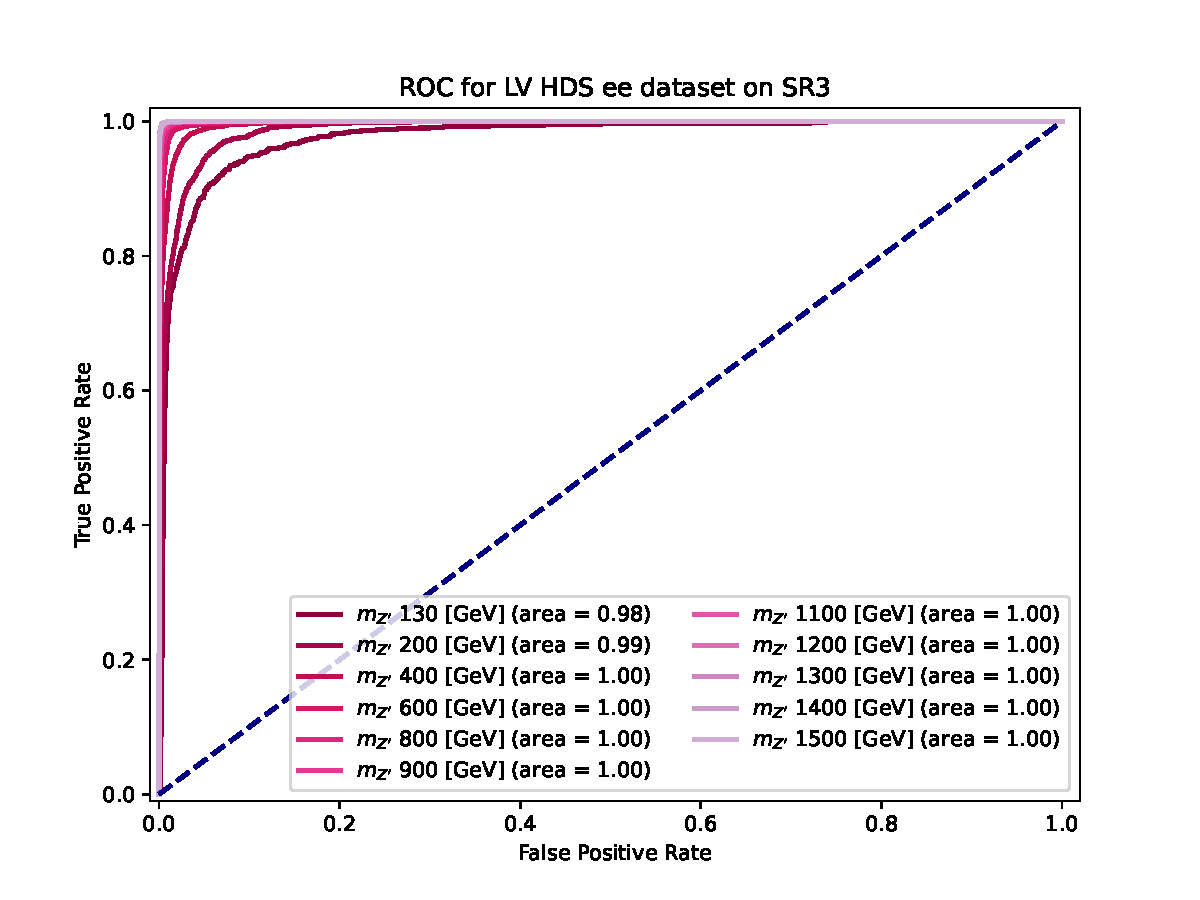
\includegraphics[width=1\textwidth]{XGBoost/Model_independent/150/LV_HDS/ROC_ee.pdf}
   \end{subfigure}
   \hfill
   \begin{subfigure}[b]{0.49\textwidth}
      \centering
      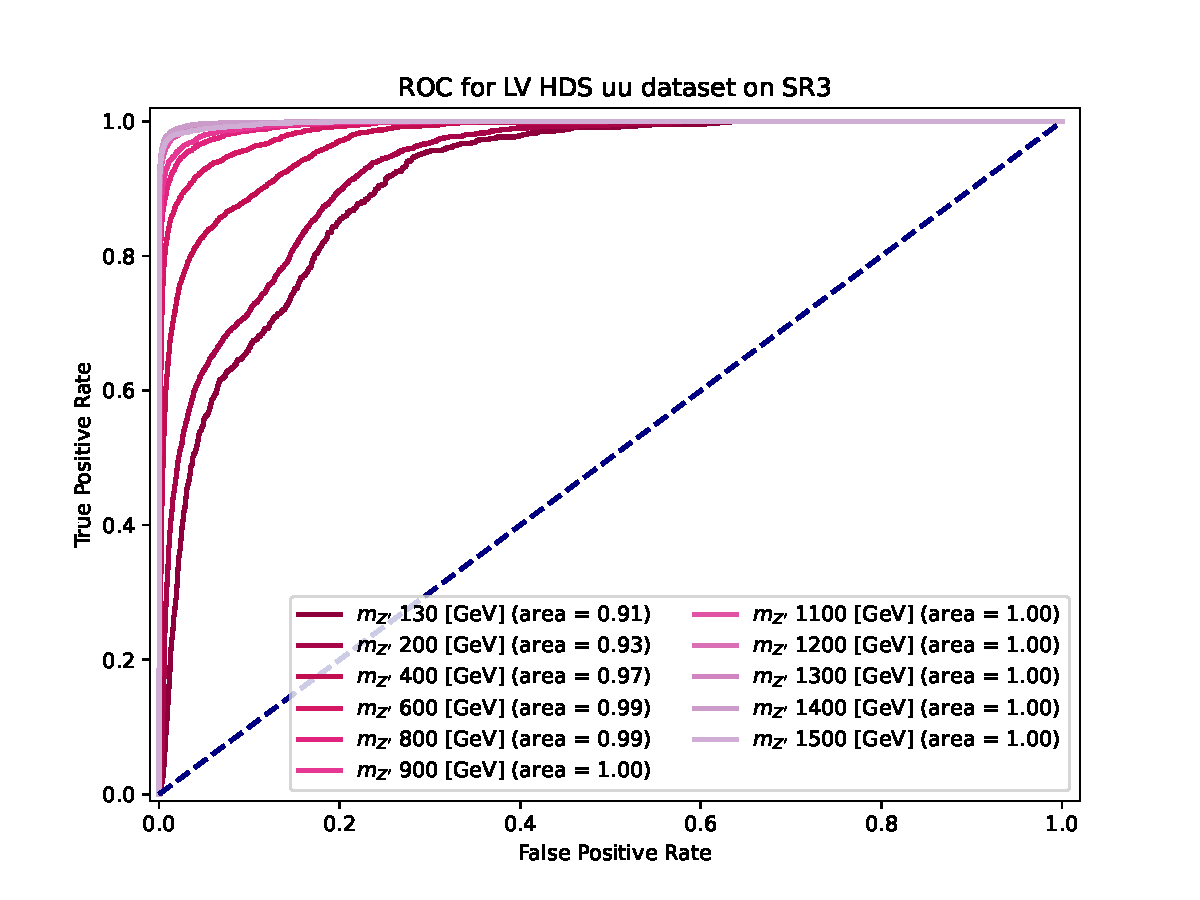
\includegraphics[width=1\textwidth]{XGBoost/Model_independent/150/LV_HDS/ROC_uu.pdf}
   \end{subfigure}
   \hfill
	\begin{subfigure}[b]{0.49\textwidth}
      \centering
      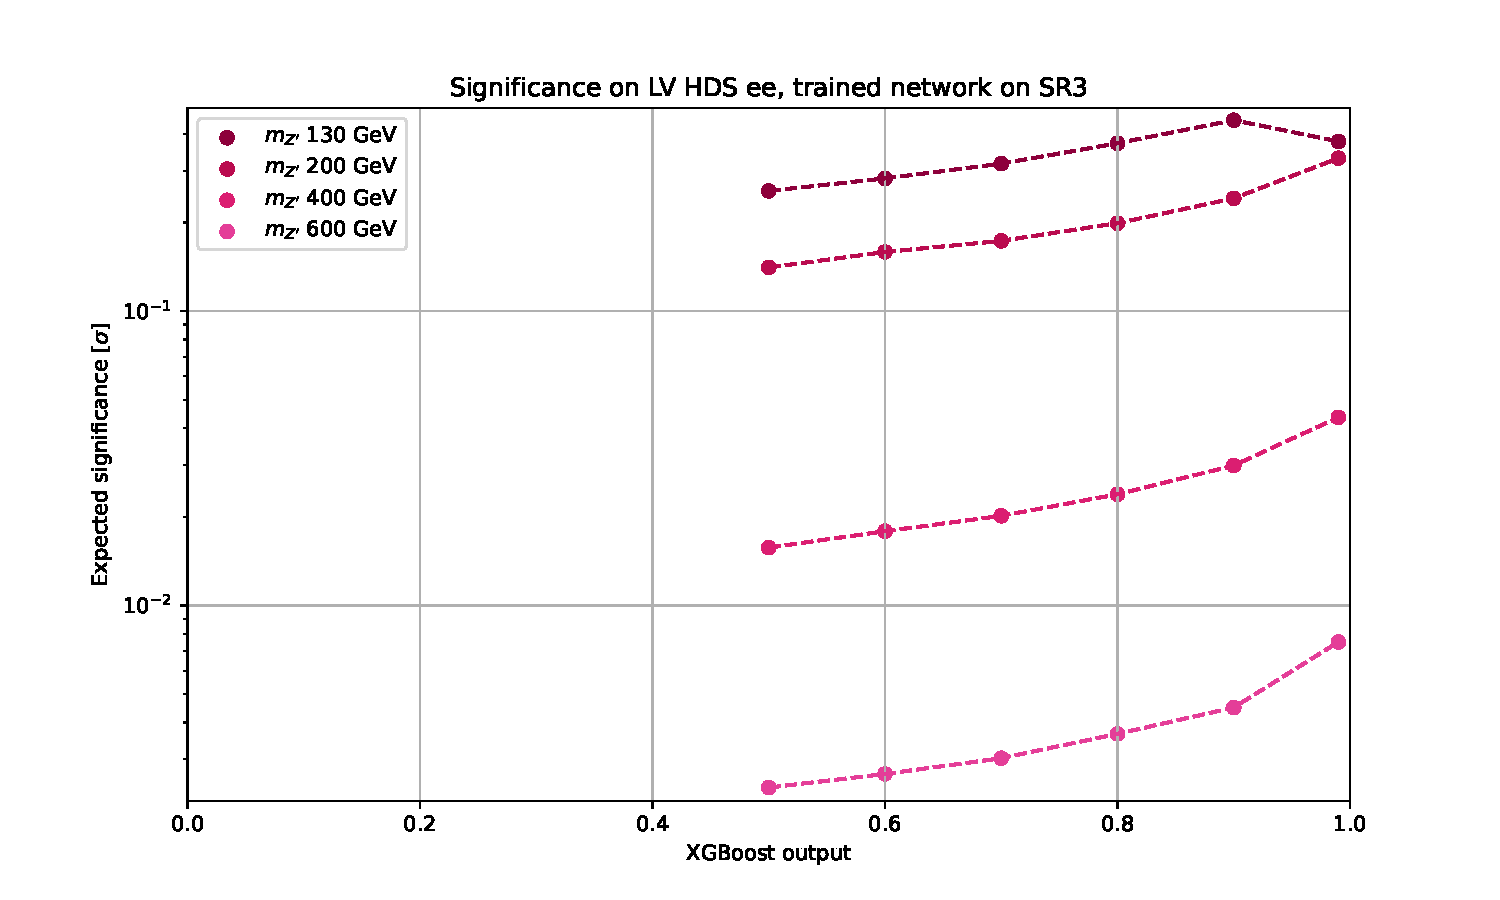
\includegraphics[width=1\textwidth]{XGBoost/Model_independent/150/LV_HDS/EXP_SIG_ee.pdf}
   \end{subfigure}
   \hfill
   \begin{subfigure}[b]{0.49\textwidth}
      \centering
      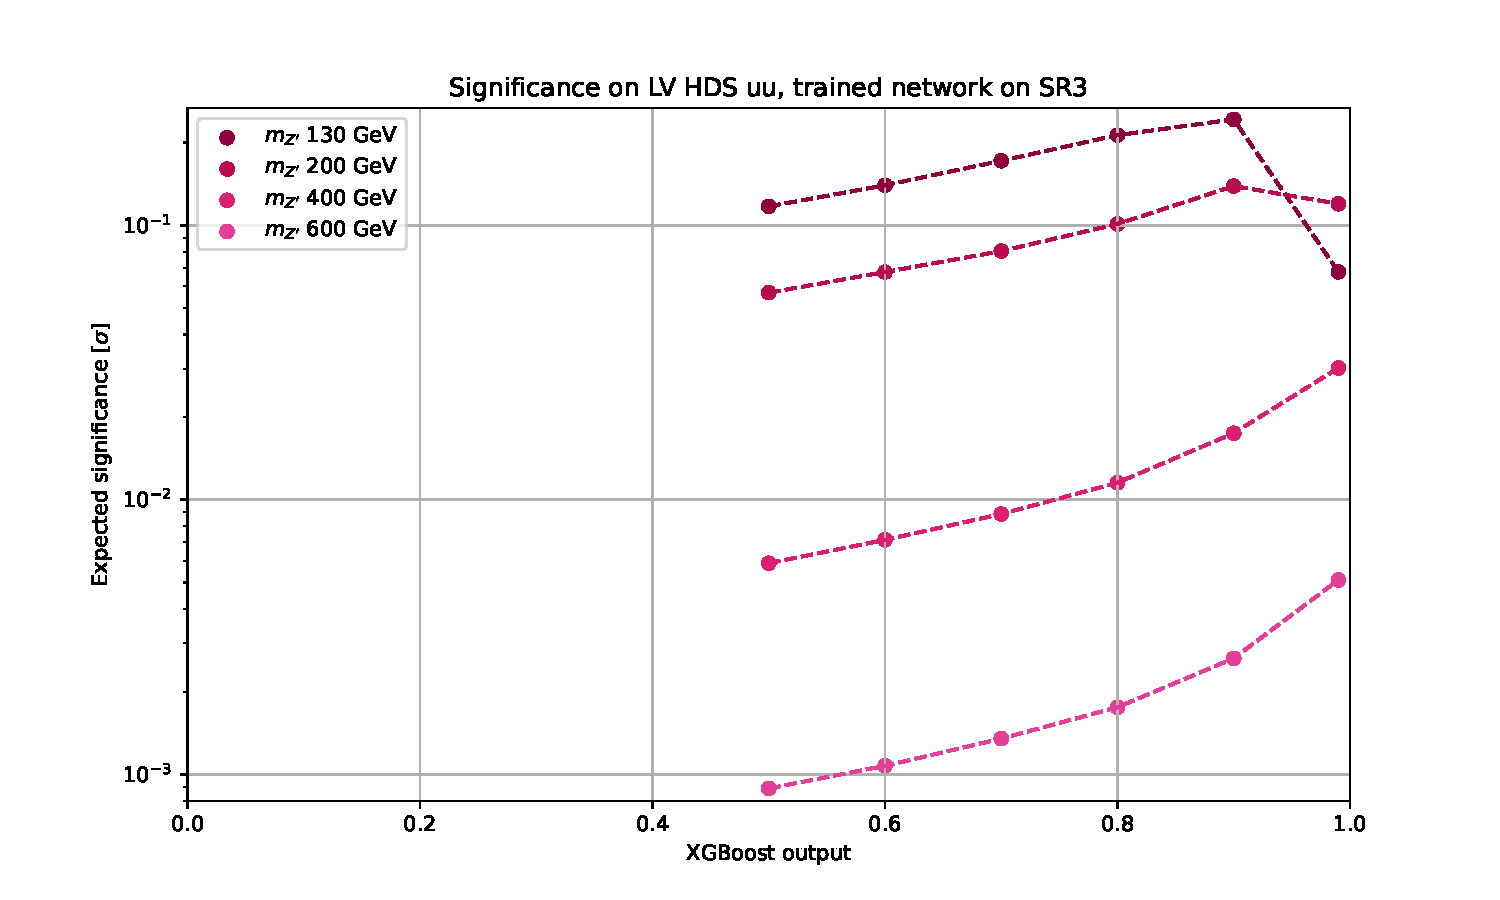
\includegraphics[width=1\textwidth]{XGBoost/Model_independent/150/LV_HDS/EXP_SIG_uu.pdf}
   \end{subfigure}
   \caption{XGBoost results for LV HDS model on $ee$ and $\mu\mu$ channel in SR3}\label{fig:LV_HDS_SR3}
\end{figure}

\begin{figure}[!ht]
	\centering
	\begin{subfigure}[b]{0.49\textwidth}
      \centering
      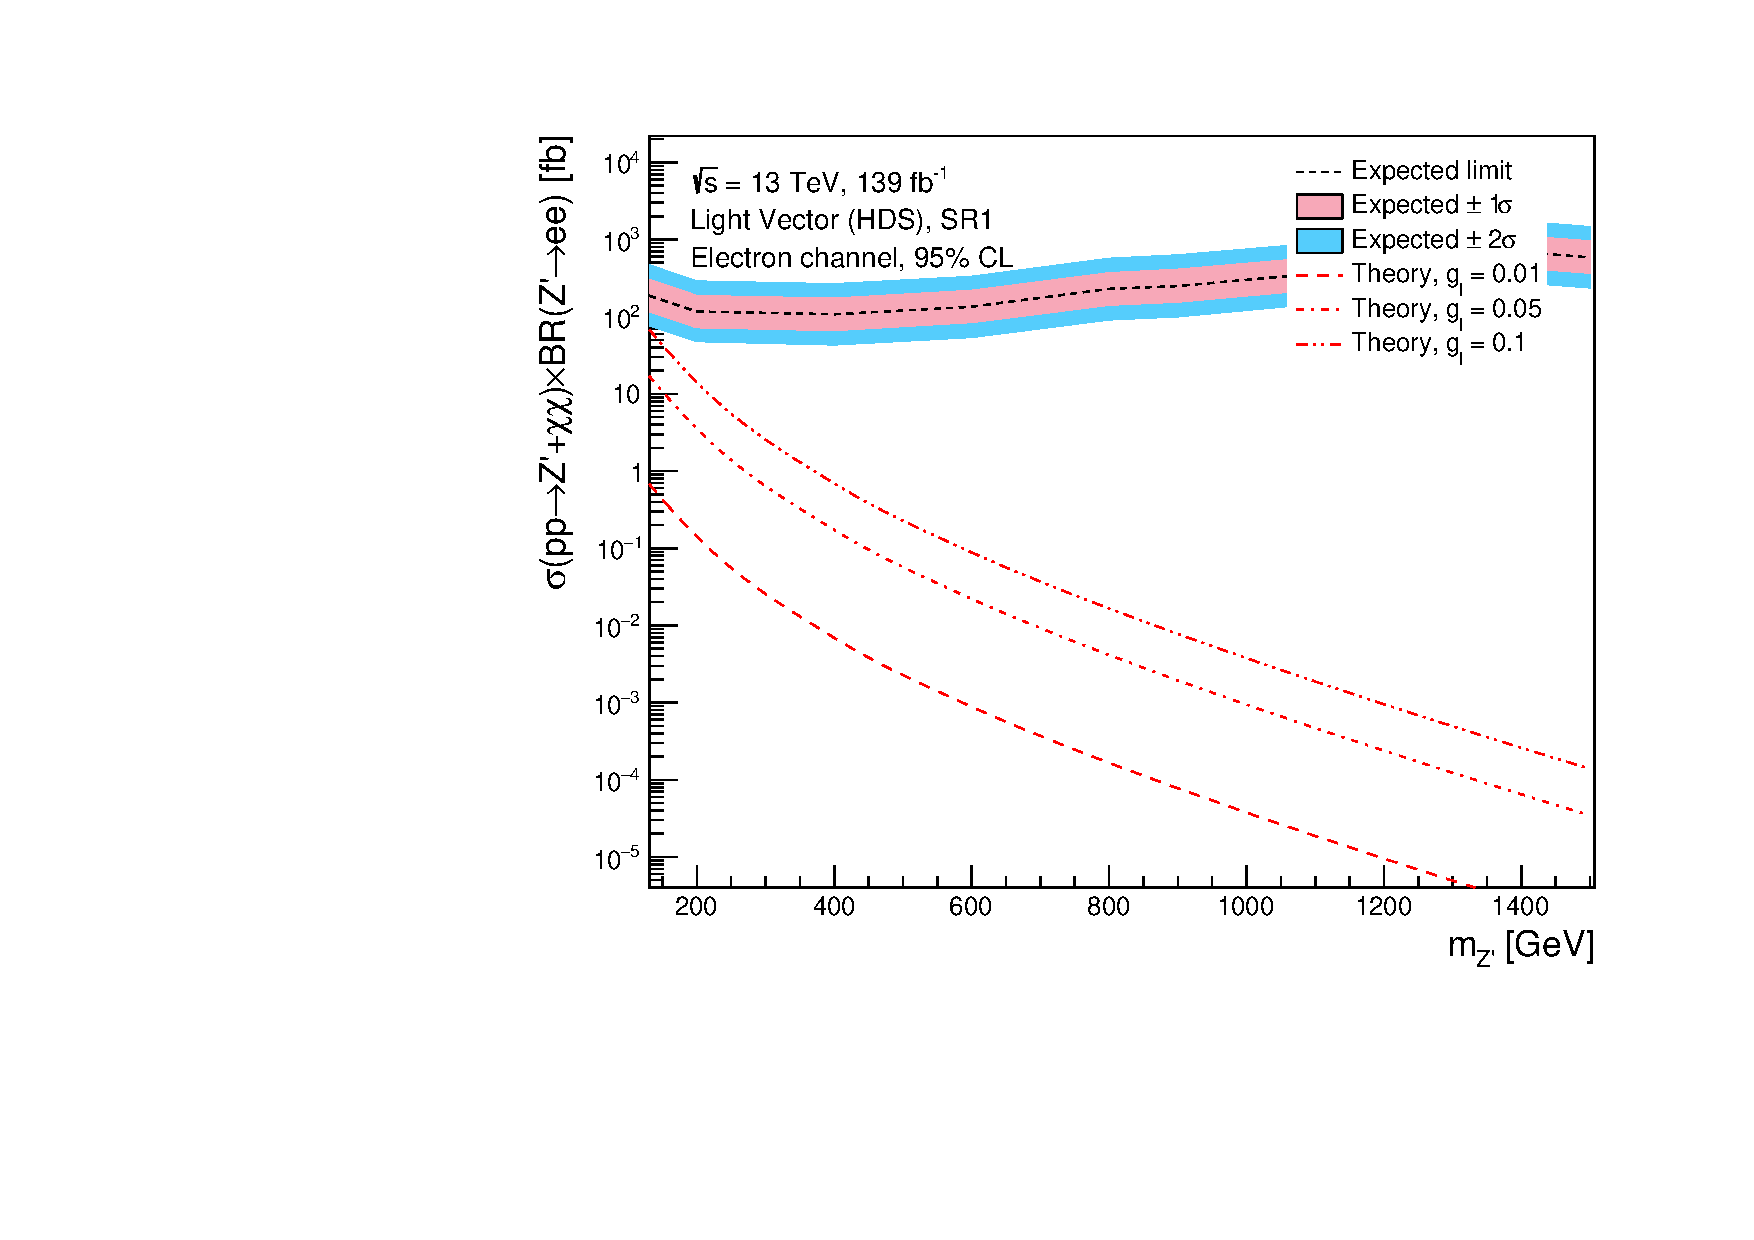
\includegraphics[width=1\textwidth]{Limits/Model_independent/50-100/LV_HDS/mass_exclusion_ee.pdf}
   \end{subfigure}
   \hfill
   \begin{subfigure}[b]{0.49\textwidth}
      \centering
      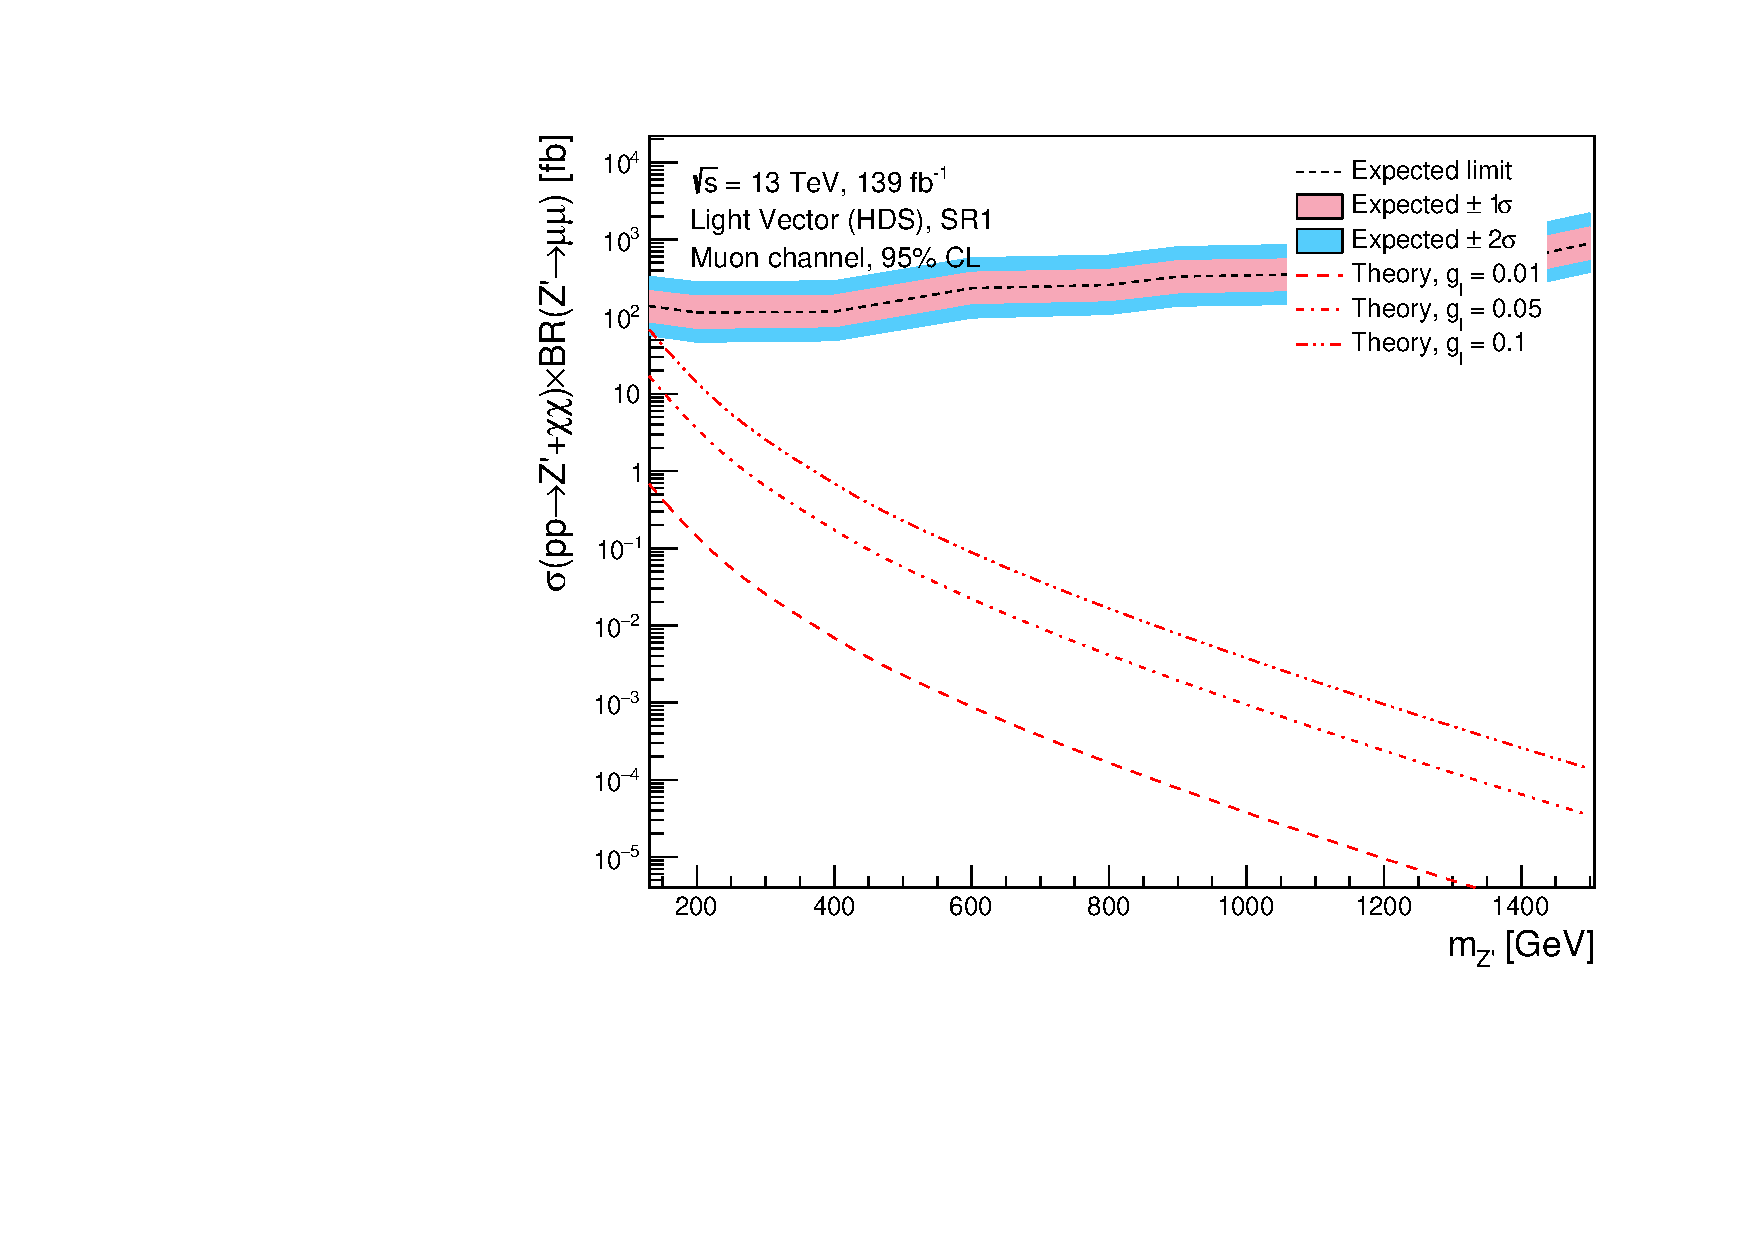
\includegraphics[width=1\textwidth]{Limits/Model_independent/50-100/LV_HDS/mass_exclusion_uu.pdf}
   \end{subfigure}
   \hfill
   \begin{subfigure}[b]{0.49\textwidth}
      \centering
      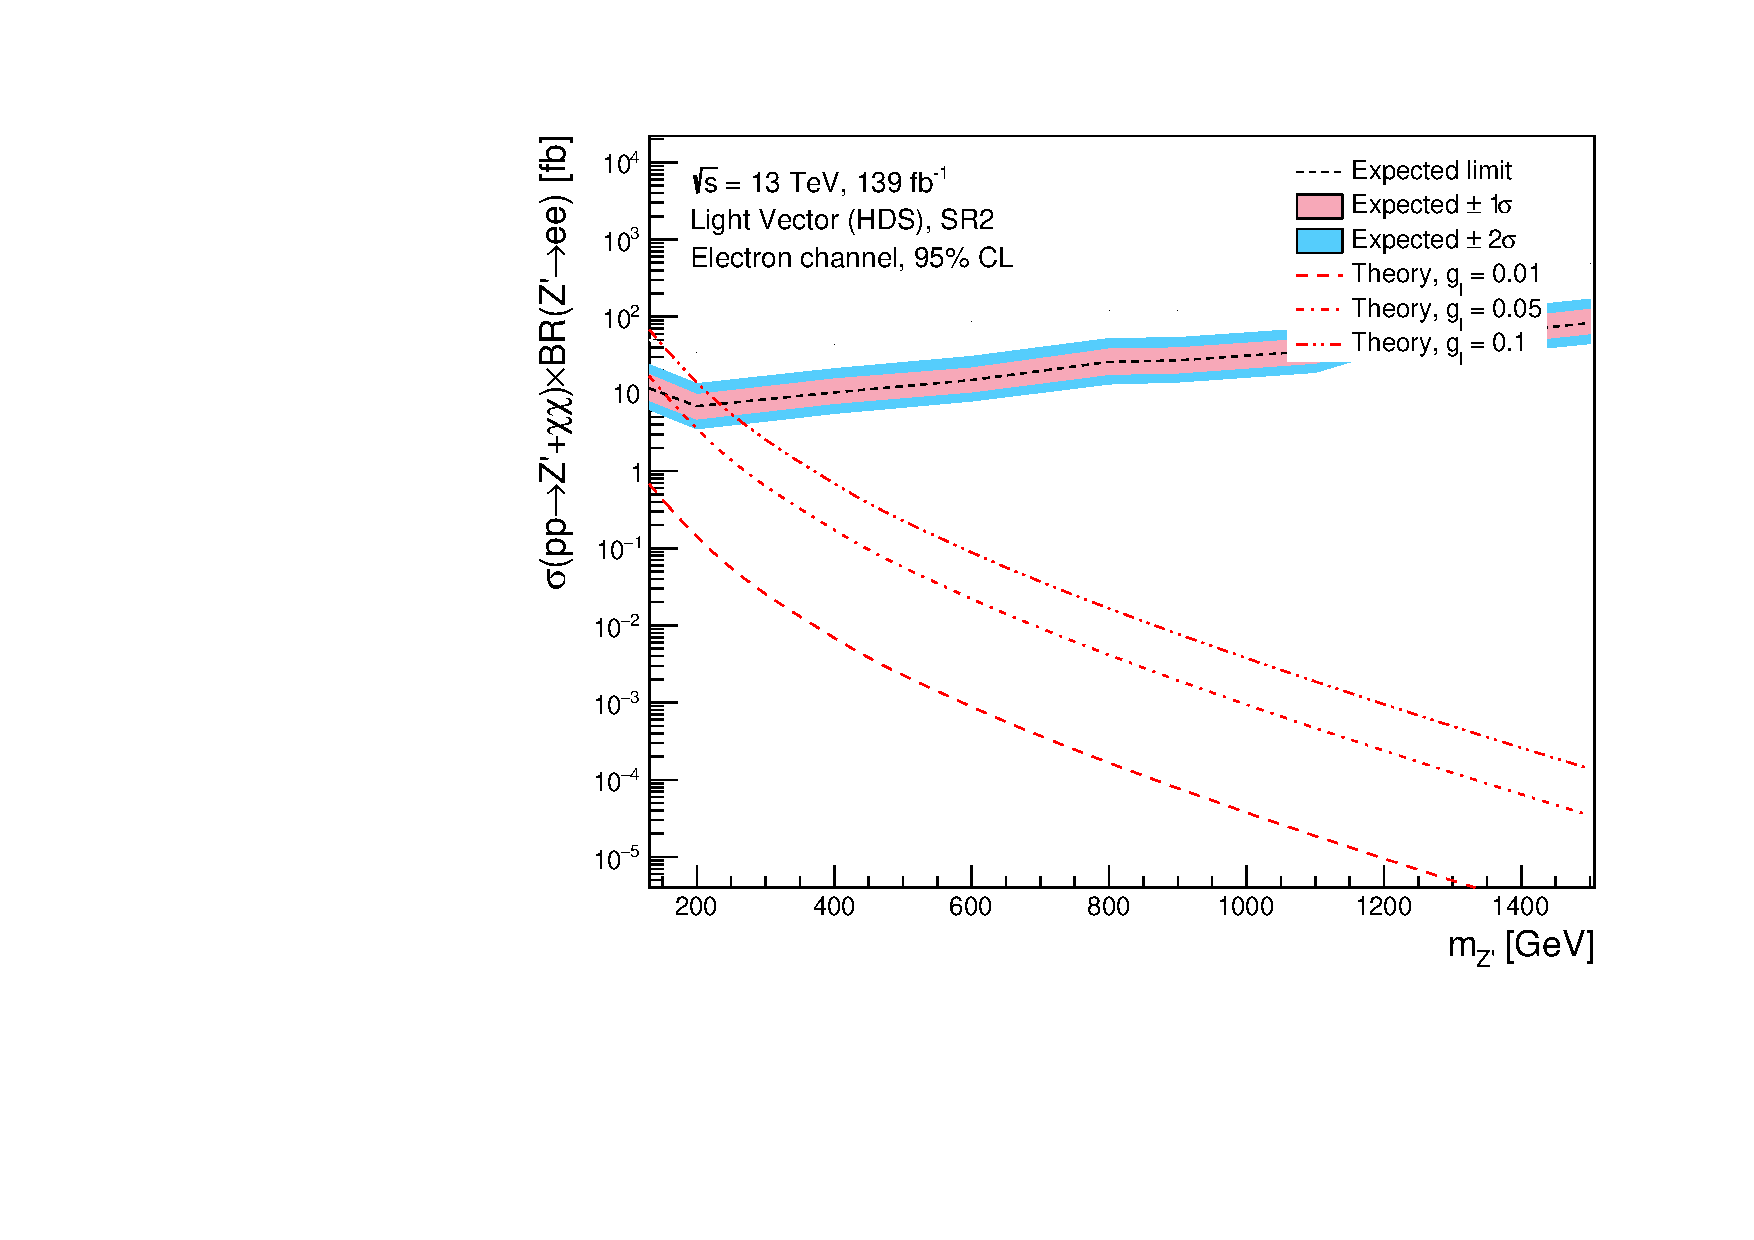
\includegraphics[width=1\textwidth]{Limits/Model_independent/100-150/LV_HDS/mass_exclusion_ee.pdf}
   \end{subfigure}
   \hfill
   \begin{subfigure}[b]{0.49\textwidth}
      \centering
      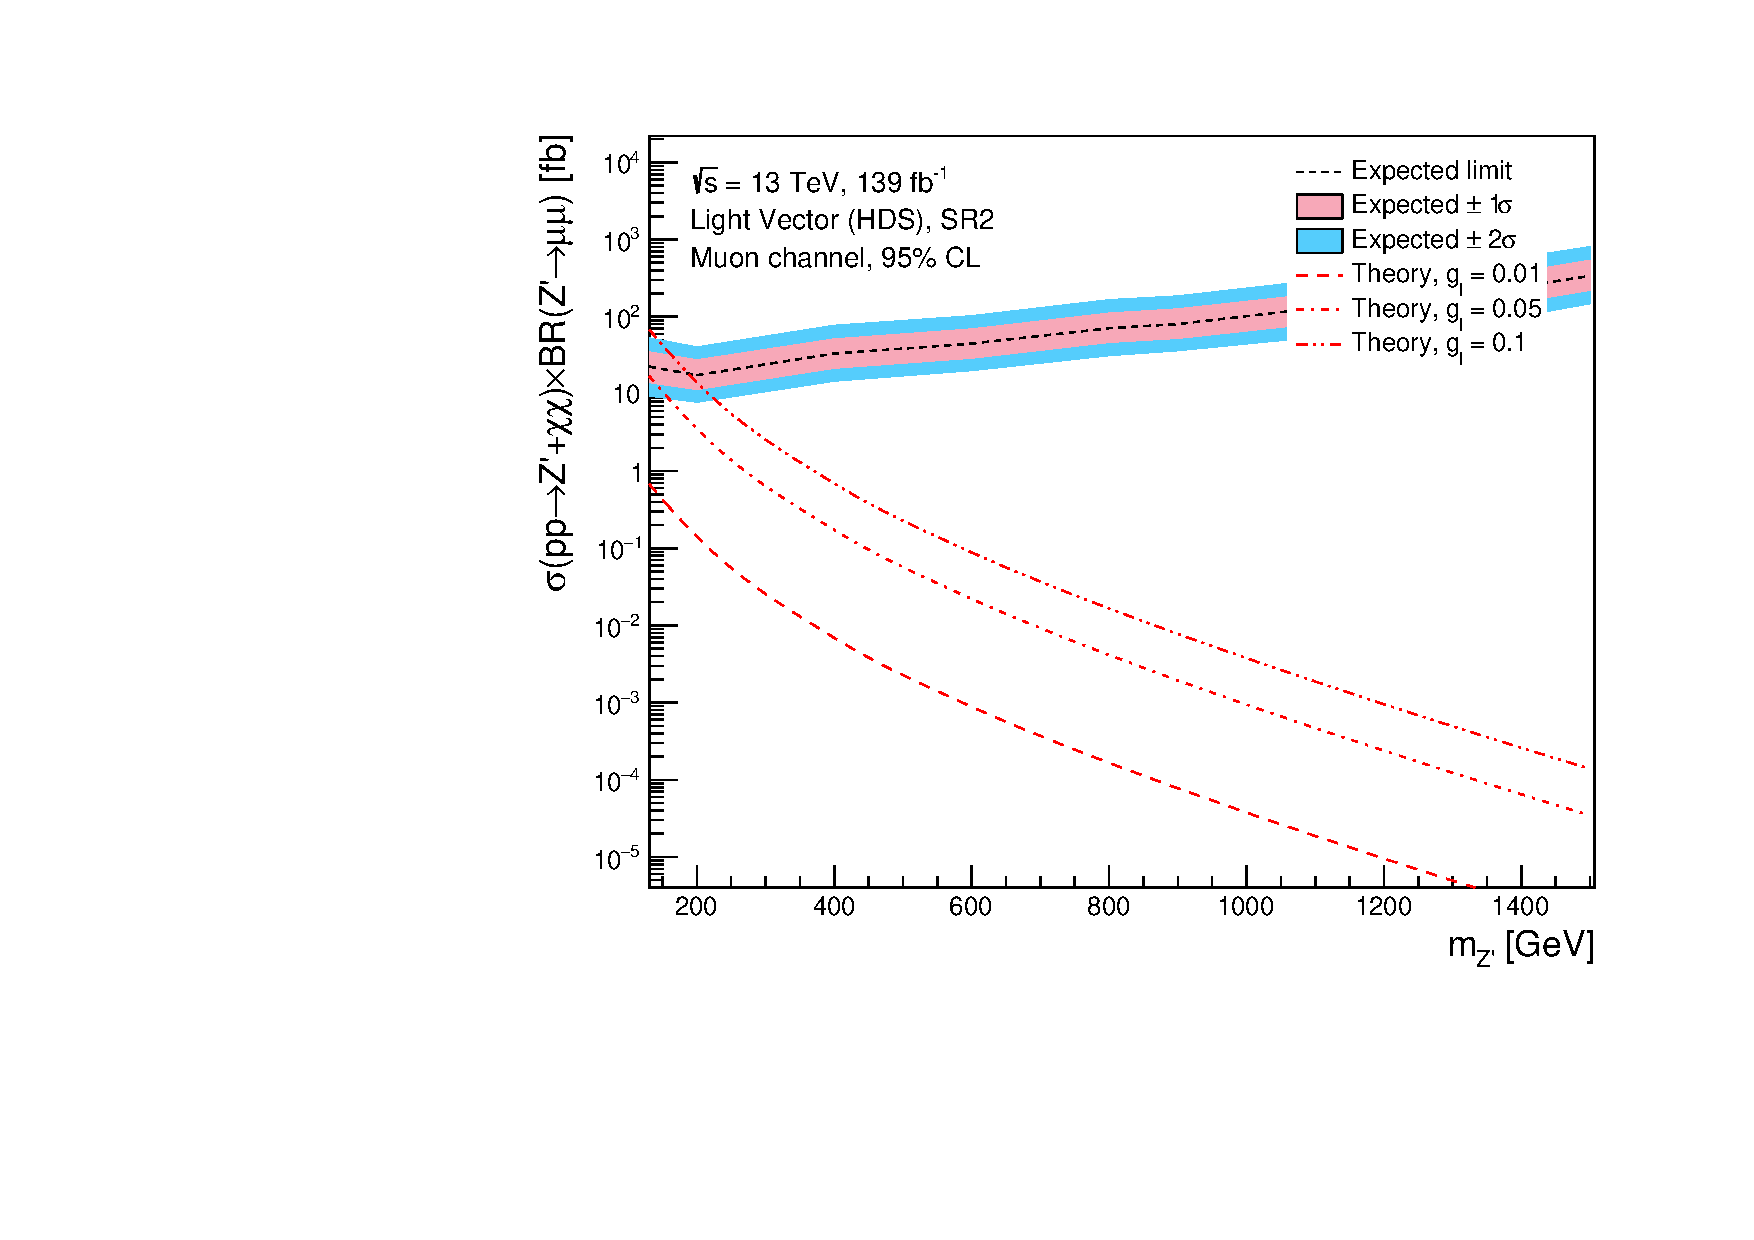
\includegraphics[width=1\textwidth]{Limits/Model_independent/100-150/LV_HDS/mass_exclusion_uu.pdf}
   \end{subfigure}
   \hfill
	\begin{subfigure}[b]{0.49\textwidth}
      \centering
      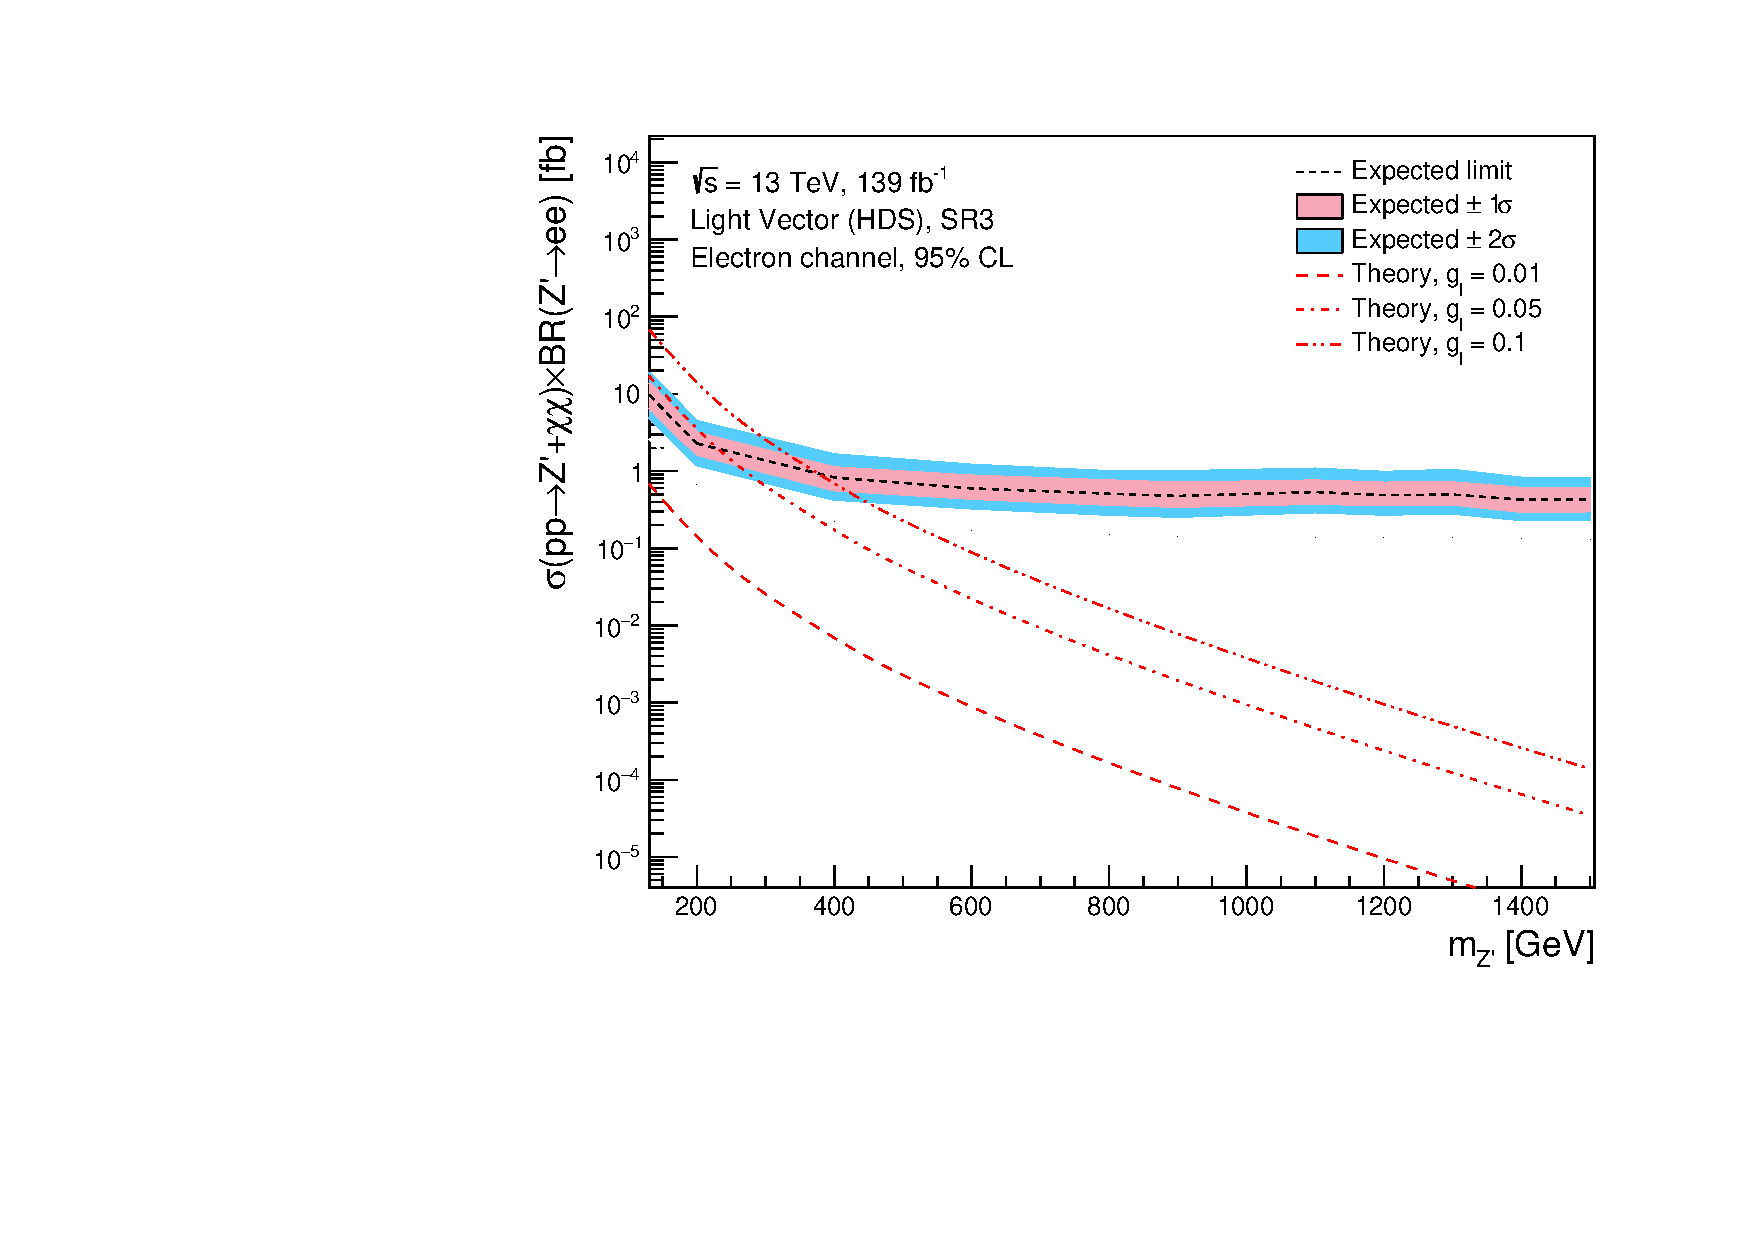
\includegraphics[width=1\textwidth]{Limits/Model_independent/150/LV_HDS/mass_exclusion_ee.pdf}
   \end{subfigure}
   \hfill
   \begin{subfigure}[b]{0.49\textwidth}
      \centering
      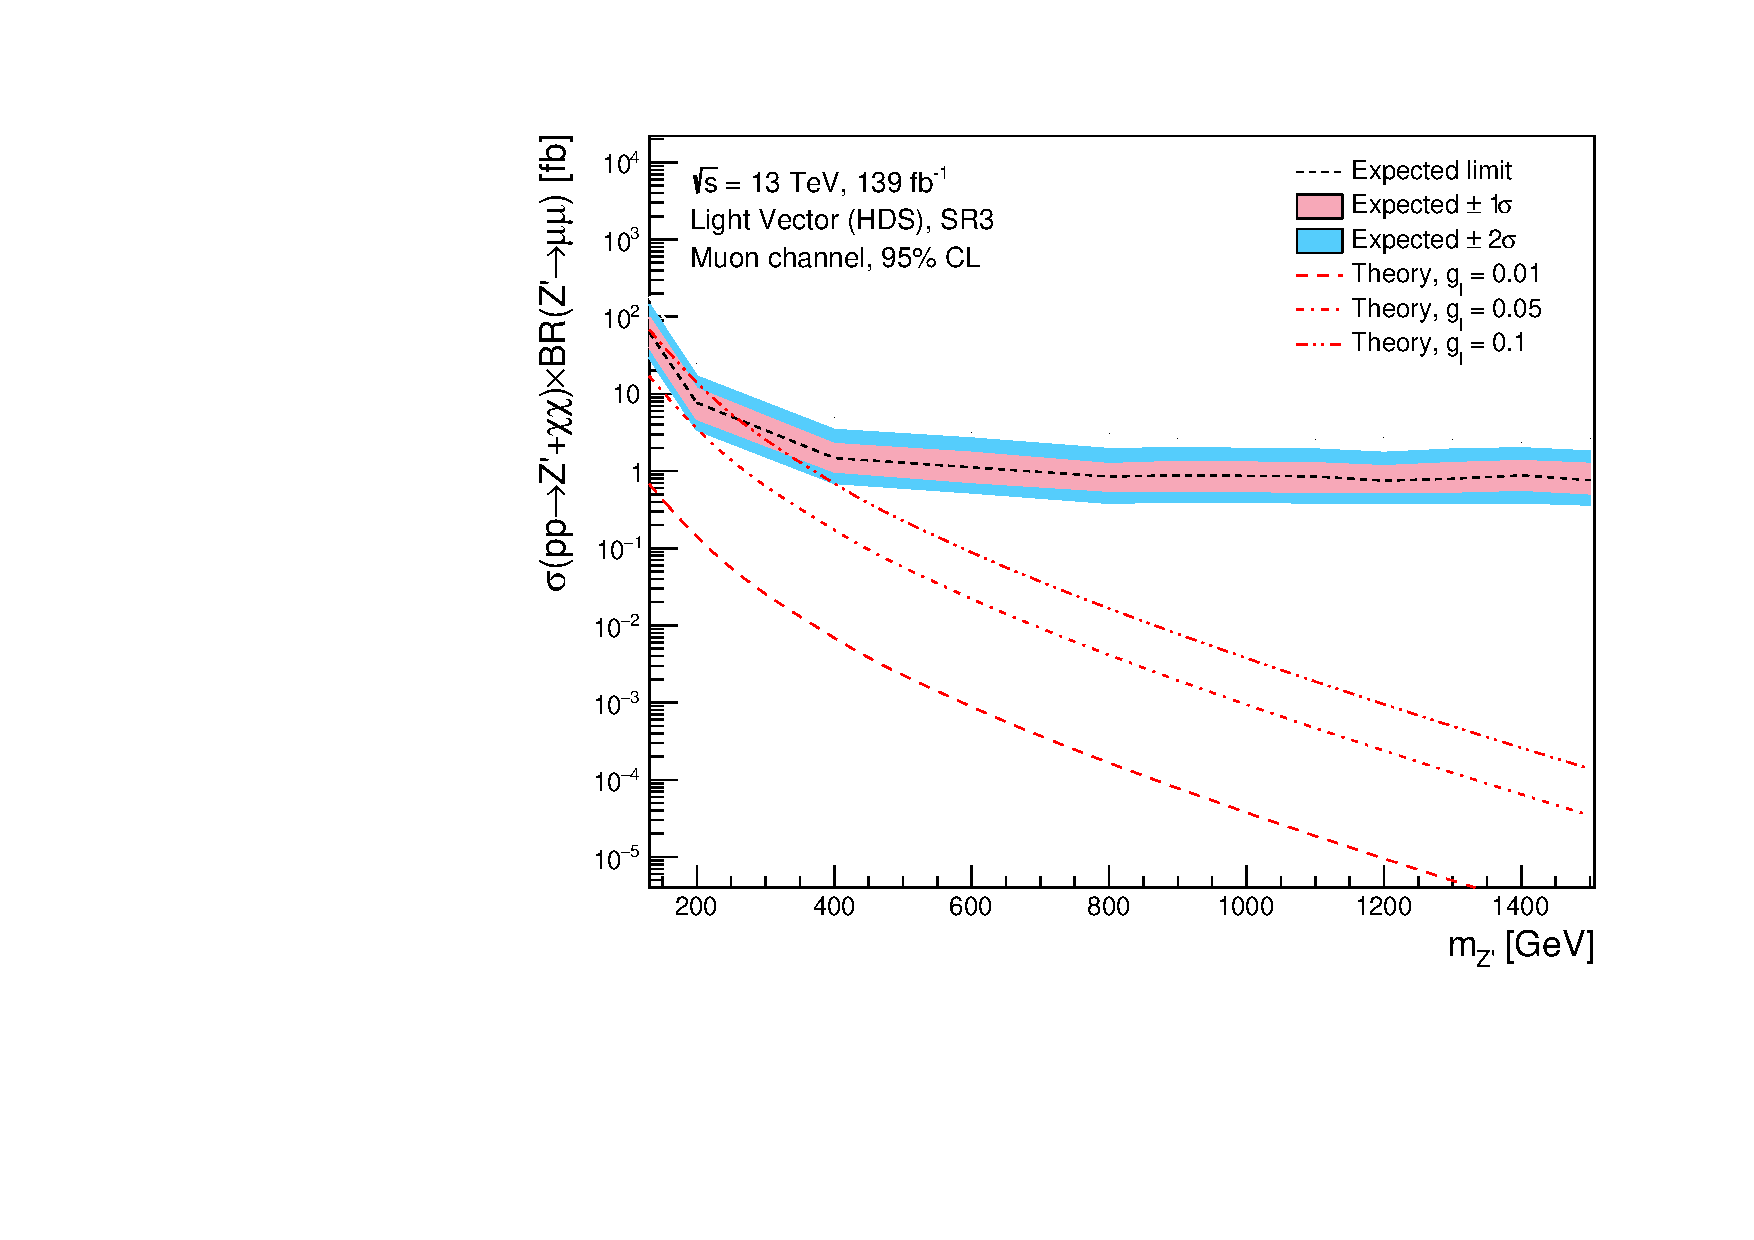
\includegraphics[width=1\textwidth]{Limits/Model_independent/150/LV_HDS/mass_exclusion_uu.pdf}
   \end{subfigure}
   \caption{Mass exclusiion limits results for LV HDS model on $ee$ and $\mu\mu$ channel in all SRs}\label{fig:LV_HDS_me_SRS}
\end{figure}

\begin{figure}[!ht]
	\centering
	\begin{subfigure}[b]{0.49\textwidth}
      \centering
      \includegraphics[width=1\textwidth]{Limits/Model_independent/LV_HDS/mass_exclusion_ee.pdf}
   \end{subfigure}
   \hfill
   \begin{subfigure}[b]{0.49\textwidth}
      \centering
      \includegraphics[width=1\textwidth]{Limits/Model_independent/LV_HDS/mass_exclusion_uu.pdf}
   \end{subfigure}
   \caption{Mass exclusiion limits results for LV HDS model on $ee$ and $\mu\mu$ channel in combined SRs}\label{fig:LV_HDS_me_comb}
\end{figure}
\clearpage
\section{Light Vector Light Dark Sector}
\begin{figure}[!ht]
	\centering
	\begin{subfigure}[b]{0.49\textwidth}
      \centering
      \includegraphics[width=1\textwidth]{XGBoost/Model_independent/50-100/LV_LDS/VAL_ee.pdf}
   \end{subfigure}
   \hfill
   \begin{subfigure}[b]{0.49\textwidth}
      \centering
      \includegraphics[width=1\textwidth]{XGBoost/Model_independent/50-100/LV_LDS/VAL_uu.pdf}
   \end{subfigure}
   \hfill
   \begin{subfigure}[b]{0.49\textwidth}
      \centering
      \includegraphics[width=1\textwidth]{XGBoost/Model_independent/50-100/LV_LDS/ROC_ee.pdf}
   \end{subfigure}
   \hfill
   \begin{subfigure}[b]{0.49\textwidth}
      \centering
      \includegraphics[width=1\textwidth]{XGBoost/Model_independent/50-100/LV_LDS/ROC_uu.pdf}
   \end{subfigure}
   \hfill
	\begin{subfigure}[b]{0.49\textwidth}
      \centering
      \includegraphics[width=1\textwidth]{XGBoost/Model_independent/50-100/LV_LDS/EXP_SIG_ee.pdf}
   \end{subfigure}
   \hfill
   \begin{subfigure}[b]{0.49\textwidth}
      \centering
      \includegraphics[width=1\textwidth]{XGBoost/Model_independent/50-100/LV_LDS/EXP_SIG_uu.pdf}
   \end{subfigure}
   \caption{XGBoost results for LV LDS model on $ee$ and $\mu\mu$ channel in SR1}\label{fig:LV_LDS_SR1}
\end{figure}

\begin{figure}[!ht]
	\centering
	\begin{subfigure}[b]{0.49\textwidth}
      \centering
      \includegraphics[width=1\textwidth]{XGBoost/Model_independent/100-150/LV_LDS/VAL_ee.pdf}
   \end{subfigure}
   \hfill
   \begin{subfigure}[b]{0.49\textwidth}
      \centering
      \includegraphics[width=1\textwidth]{XGBoost/Model_independent/100-150/LV_LDS/VAL_uu.pdf}
   \end{subfigure}
   \hfill
   \begin{subfigure}[b]{0.49\textwidth}
      \centering
      \includegraphics[width=1\textwidth]{XGBoost/Model_independent/100-150/LV_LDS/ROC_ee.pdf}
   \end{subfigure}
   \hfill
   \begin{subfigure}[b]{0.49\textwidth}
      \centering
      \includegraphics[width=1\textwidth]{XGBoost/Model_independent/100-150/LV_LDS/ROC_uu.pdf}
   \end{subfigure}
   \hfill
	\begin{subfigure}[b]{0.49\textwidth}
      \centering
      \includegraphics[width=1\textwidth]{XGBoost/Model_independent/100-150/LV_LDS/EXP_SIG_ee.pdf}
   \end{subfigure}
   \hfill
   \begin{subfigure}[b]{0.49\textwidth}
      \centering
      \includegraphics[width=1\textwidth]{XGBoost/Model_independent/100-150/LV_LDS/EXP_SIG_uu.pdf}
   \end{subfigure}
   \caption{XGBoost results for LV LDS model on $ee$ and $\mu\mu$ channel in SR2}\label{fig:LV_LDS_SR2}
\end{figure}

\begin{figure}[!ht]
	\centering
	\begin{subfigure}[b]{0.49\textwidth}
      \centering
      \includegraphics[width=1\textwidth]{XGBoost/Model_independent/150/LV_LDS/VAL_ee.pdf}
   \end{subfigure}
   \hfill
   \begin{subfigure}[b]{0.49\textwidth}
      \centering
      \includegraphics[width=1\textwidth]{XGBoost/Model_independent/150/LV_LDS/VAL_uu.pdf}
   \end{subfigure}
   \hfill
   \begin{subfigure}[b]{0.49\textwidth}
      \centering
      \includegraphics[width=1\textwidth]{XGBoost/Model_independent/150/LV_LDS/ROC_ee.pdf}
   \end{subfigure}
   \hfill
   \begin{subfigure}[b]{0.49\textwidth}
      \centering
      \includegraphics[width=1\textwidth]{XGBoost/Model_independent/150/LV_LDS/ROC_uu.pdf}
   \end{subfigure}
   \hfill
	\begin{subfigure}[b]{0.49\textwidth}
      \centering
      \includegraphics[width=1\textwidth]{XGBoost/Model_independent/150/LV_LDS/EXP_SIG_ee.pdf}
   \end{subfigure}
   \hfill
   \begin{subfigure}[b]{0.49\textwidth}
      \centering
      \includegraphics[width=1\textwidth]{XGBoost/Model_independent/150/LV_LDS/EXP_SIG_uu.pdf}
   \end{subfigure}
   \caption{XGBoost results for LV LDS model on $ee$ and $\mu\mu$ channel in SR3}\label{fig:LV_LDS_SR3}
\end{figure}

\begin{figure}[!ht]
	\centering
	\begin{subfigure}[b]{0.49\textwidth}
      \centering
      \includegraphics[width=1\textwidth]{Limits/Model_independent/50-100/LV_LDS/mass_exclusion_ee.pdf}
   \end{subfigure}
   \hfill
   \begin{subfigure}[b]{0.49\textwidth}
      \centering
      \includegraphics[width=1\textwidth]{Limits/Model_independent/50-100/LV_LDS/mass_exclusion_uu.pdf}
   \end{subfigure}
   \hfill
   \begin{subfigure}[b]{0.49\textwidth}
      \centering
      \includegraphics[width=1\textwidth]{Limits/Model_independent/100-150/LV_LDS/mass_exclusion_ee.pdf}
   \end{subfigure}
   \hfill
   \begin{subfigure}[b]{0.49\textwidth}
      \centering
      \includegraphics[width=1\textwidth]{Limits/Model_independent/100-150/LV_LDS/mass_exclusion_uu.pdf}
   \end{subfigure}
   \hfill
	\begin{subfigure}[b]{0.49\textwidth}
      \centering
      \includegraphics[width=1\textwidth]{Limits/Model_independent/150/LV_LDS/mass_exclusion_ee.pdf}
   \end{subfigure}
   \hfill
   \begin{subfigure}[b]{0.49\textwidth}
      \centering
      \includegraphics[width=1\textwidth]{Limits/Model_independent/150/LV_LDS/mass_exclusion_uu.pdf}
   \end{subfigure}
   \caption{Mass exclusiion limits results for LV LDS model on $ee$ and $\mu\mu$ channel in all SRs}\label{fig:LV_LDS_me_SRS}
\end{figure}

\begin{figure}[!ht]
	\centering
	\begin{subfigure}[b]{0.49\textwidth}
      \centering
      \includegraphics[width=1\textwidth]{Limits/Model_independent/LV_LDS/mass_exclusion_ee.pdf}
   \end{subfigure}
   \hfill
   \begin{subfigure}[b]{0.49\textwidth}
      \centering
      \includegraphics[width=1\textwidth]{Limits/Model_independent/LV_LDS/mass_exclusion_uu.pdf}
   \end{subfigure}
   \caption{Mass exclusiion limits results for LV LDS model on $ee$ and $\mu\mu$ channel in combined SRs}\label{fig:LV_LDS_me_comb}
\end{figure}
\clearpage
\section{Effective Field Theory Heavy Dark Sector}
\begin{figure}[!ht]
	\centering
	\begin{subfigure}[b]{0.49\textwidth}
      \centering
      \includegraphics[width=1\textwidth]{XGBoost/Model_independent/50-100/EFT_HDS/VAL_ee.pdf}
   \end{subfigure}
   \hfill
   \begin{subfigure}[b]{0.49\textwidth}
      \centering
      \includegraphics[width=1\textwidth]{XGBoost/Model_independent/50-100/EFT_HDS/VAL_uu.pdf}
   \end{subfigure}
   \hfill
   \begin{subfigure}[b]{0.49\textwidth}
      \centering
      \includegraphics[width=1\textwidth]{XGBoost/Model_independent/50-100/EFT_HDS/ROC_ee.pdf}
   \end{subfigure}
   \hfill
   \begin{subfigure}[b]{0.49\textwidth}
      \centering
      \includegraphics[width=1\textwidth]{XGBoost/Model_independent/50-100/EFT_HDS/ROC_uu.pdf}
   \end{subfigure}
   \hfill
	\begin{subfigure}[b]{0.49\textwidth}
      \centering
      \includegraphics[width=1\textwidth]{XGBoost/Model_independent/50-100/EFT_HDS/EXP_SIG_ee.pdf}
   \end{subfigure}
   \hfill
   \begin{subfigure}[b]{0.49\textwidth}
      \centering
      \includegraphics[width=1\textwidth]{XGBoost/Model_independent/50-100/EFT_HDS/EXP_SIG_uu.pdf}
   \end{subfigure}
   \caption{XGBoost results for EFT HDS model on $ee$ and $\mu\mu$ channel in SR1}\label{fig:EFT_HDS_SR1}
\end{figure}

\begin{figure}[!ht]
	\centering
	\begin{subfigure}[b]{0.49\textwidth}
      \centering
      \includegraphics[width=1\textwidth]{XGBoost/Model_independent/100-150/EFT_HDS/VAL_ee.pdf}
   \end{subfigure}
   \hfill
   \begin{subfigure}[b]{0.49\textwidth}
      \centering
      \includegraphics[width=1\textwidth]{XGBoost/Model_independent/100-150/EFT_HDS/VAL_uu.pdf}
   \end{subfigure}
   \hfill
   \begin{subfigure}[b]{0.49\textwidth}
      \centering
      \includegraphics[width=1\textwidth]{XGBoost/Model_independent/100-150/EFT_HDS/ROC_ee.pdf}
   \end{subfigure}
   \hfill
   \begin{subfigure}[b]{0.49\textwidth}
      \centering
      \includegraphics[width=1\textwidth]{XGBoost/Model_independent/100-150/EFT_HDS/ROC_uu.pdf}
   \end{subfigure}
   \hfill
	\begin{subfigure}[b]{0.49\textwidth}
      \centering
      \includegraphics[width=1\textwidth]{XGBoost/Model_independent/100-150/EFT_HDS/EXP_SIG_ee.pdf}
   \end{subfigure}
   \hfill
   \begin{subfigure}[b]{0.49\textwidth}
      \centering
      \includegraphics[width=1\textwidth]{XGBoost/Model_independent/100-150/EFT_HDS/EXP_SIG_uu.pdf}
   \end{subfigure}
   \caption{XGBoost results for EFT HDS model on $ee$ and $\mu\mu$ channel in SR2}\label{fig:EFT_HDS_SR2}
\end{figure}

\begin{figure}[!ht]
	\centering
	\begin{subfigure}[b]{0.49\textwidth}
      \centering
      \includegraphics[width=1\textwidth]{XGBoost/Model_independent/150/EFT_HDS/VAL_ee.pdf}
   \end{subfigure}
   \hfill
   \begin{subfigure}[b]{0.49\textwidth}
      \centering
      \includegraphics[width=1\textwidth]{XGBoost/Model_independent/150/EFT_HDS/VAL_uu.pdf}
   \end{subfigure}
   \hfill
   \begin{subfigure}[b]{0.49\textwidth}
      \centering
      \includegraphics[width=1\textwidth]{XGBoost/Model_independent/150/EFT_HDS/ROC_ee.pdf}
   \end{subfigure}
   \hfill
   \begin{subfigure}[b]{0.49\textwidth}
      \centering
      \includegraphics[width=1\textwidth]{XGBoost/Model_independent/150/EFT_HDS/ROC_uu.pdf}
   \end{subfigure}
   \hfill
	\begin{subfigure}[b]{0.49\textwidth}
      \centering
      \includegraphics[width=1\textwidth]{XGBoost/Model_independent/150/EFT_HDS/EXP_SIG_ee.pdf}
   \end{subfigure}
   \hfill
   \begin{subfigure}[b]{0.49\textwidth}
      \centering
      \includegraphics[width=1\textwidth]{XGBoost/Model_independent/150/EFT_HDS/EXP_SIG_uu.pdf}
   \end{subfigure}
   \caption{XGBoost results for EFT HDS model on $ee$ and $\mu\mu$ channel in SR3}\label{fig:EFT_HDS_SR3}
\end{figure}

\begin{figure}[!ht]
	\centering
	\begin{subfigure}[b]{0.49\textwidth}
      \centering
      \includegraphics[width=1\textwidth]{Limits/Model_independent/50-100/EFT_HDS/mass_exclusion_ee.pdf}
   \end{subfigure}
   \hfill
   \begin{subfigure}[b]{0.49\textwidth}
      \centering
      \includegraphics[width=1\textwidth]{Limits/Model_independent/50-100/EFT_HDS/mass_exclusion_uu.pdf}
   \end{subfigure}
   \hfill
   \begin{subfigure}[b]{0.49\textwidth}
      \centering
      \includegraphics[width=1\textwidth]{Limits/Model_independent/100-150/EFT_HDS/mass_exclusion_ee.pdf}
   \end{subfigure}
   \hfill
   \begin{subfigure}[b]{0.49\textwidth}
      \centering
      \includegraphics[width=1\textwidth]{Limits/Model_independent/100-150/EFT_HDS/mass_exclusion_uu.pdf}
   \end{subfigure}
   \hfill
	\begin{subfigure}[b]{0.49\textwidth}
      \centering
      \includegraphics[width=1\textwidth]{Limits/Model_independent/150/EFT_HDS/mass_exclusion_ee.pdf}
   \end{subfigure}
   \hfill
   \begin{subfigure}[b]{0.49\textwidth}
      \centering
      \includegraphics[width=1\textwidth]{Limits/Model_independent/150/EFT_HDS/mass_exclusion_uu.pdf}
   \end{subfigure}
   \caption{Mass exclusiion limits results for EFT HDS model on $ee$ and $\mu\mu$ channel in all SRs}\label{fig:EFT_HDS_me_SRS}
\end{figure}

\begin{figure}[!ht]
	\centering
	\begin{subfigure}[b]{0.49\textwidth}
      \centering
      \includegraphics[width=1\textwidth]{Limits/Model_independent/EFT_HDS/mass_exclusion_ee.pdf}
   \end{subfigure}
   \hfill
   \begin{subfigure}[b]{0.49\textwidth}
      \centering
      \includegraphics[width=1\textwidth]{Limits/Model_independent/EFT_HDS/mass_exclusion_uu.pdf}
   \end{subfigure}
   \caption{Mass exclusiion limits results for EFT HDS model on $ee$ and $\mu\mu$ channel in combined SRs}\label{fig:EFT_HDS_me_comb}
\end{figure}
\clearpage


\section{Effective Field Theory Light Dark Sector}
\begin{figure}[!ht]
	\centering
	\begin{subfigure}[b]{0.49\textwidth}
      \centering
      \includegraphics[width=1\textwidth]{XGBoost/Model_independent/50-100/EFT_LDS/VAL_ee.pdf}
   \end{subfigure}
   \hfill
   \begin{subfigure}[b]{0.49\textwidth}
      \centering
      \includegraphics[width=1\textwidth]{XGBoost/Model_independent/50-100/EFT_LDS/VAL_uu.pdf}
   \end{subfigure}
   \hfill
   \begin{subfigure}[b]{0.49\textwidth}
      \centering
      \includegraphics[width=1\textwidth]{XGBoost/Model_independent/50-100/EFT_LDS/ROC_ee.pdf}
   \end{subfigure}
   \hfill
   \begin{subfigure}[b]{0.49\textwidth}
      \centering
      \includegraphics[width=1\textwidth]{XGBoost/Model_independent/50-100/EFT_LDS/ROC_uu.pdf}
   \end{subfigure}
   \hfill
	\begin{subfigure}[b]{0.49\textwidth}
      \centering
      \includegraphics[width=1\textwidth]{XGBoost/Model_independent/50-100/EFT_LDS/EXP_SIG_ee.pdf}
   \end{subfigure}
   \hfill
   \begin{subfigure}[b]{0.49\textwidth}
      \centering
      \includegraphics[width=1\textwidth]{XGBoost/Model_independent/50-100/EFT_LDS/EXP_SIG_uu.pdf}
   \end{subfigure}
   \caption{XGBoost results for EFT LDS model on $ee$ and $\mu\mu$ channel in SR1}\label{fig:EFT_LDS_SR1}
\end{figure}

\begin{figure}[!ht]
	\centering
	\begin{subfigure}[b]{0.49\textwidth}
      \centering
      \includegraphics[width=1\textwidth]{XGBoost/Model_independent/100-150/EFT_LDS/VAL_ee.pdf}
   \end{subfigure}
   \hfill
   \begin{subfigure}[b]{0.49\textwidth}
      \centering
      \includegraphics[width=1\textwidth]{XGBoost/Model_independent/100-150/EFT_LDS/VAL_uu.pdf}
   \end{subfigure}
   \hfill
   \begin{subfigure}[b]{0.49\textwidth}
      \centering
      \includegraphics[width=1\textwidth]{XGBoost/Model_independent/100-150/EFT_LDS/ROC_ee.pdf}
   \end{subfigure}
   \hfill
   \begin{subfigure}[b]{0.49\textwidth}
      \centering
      \includegraphics[width=1\textwidth]{XGBoost/Model_independent/100-150/EFT_LDS/ROC_uu.pdf}
   \end{subfigure}
   \hfill
	\begin{subfigure}[b]{0.49\textwidth}
      \centering
      \includegraphics[width=1\textwidth]{XGBoost/Model_independent/100-150/EFT_LDS/EXP_SIG_ee.pdf}
   \end{subfigure}
   \hfill
   \begin{subfigure}[b]{0.49\textwidth}
      \centering
      \includegraphics[width=1\textwidth]{XGBoost/Model_independent/100-150/EFT_LDS/EXP_SIG_uu.pdf}
   \end{subfigure}
   \caption{XGBoost results for EFT LDS model on $ee$ and $\mu\mu$ channel in SR2}\label{fig:EFT_LDS_SR2}
\end{figure}

\begin{figure}[!ht]
	\centering
	\begin{subfigure}[b]{0.49\textwidth}
      \centering
      \includegraphics[width=1\textwidth]{XGBoost/Model_independent/150/EFT_LDS/VAL_ee.pdf}
   \end{subfigure}
   \hfill
   \begin{subfigure}[b]{0.49\textwidth}
      \centering
      \includegraphics[width=1\textwidth]{XGBoost/Model_independent/150/EFT_LDS/VAL_uu.pdf}
   \end{subfigure}
   \hfill
   \begin{subfigure}[b]{0.49\textwidth}
      \centering
      \includegraphics[width=1\textwidth]{XGBoost/Model_independent/150/EFT_LDS/ROC_ee.pdf}
   \end{subfigure}
   \hfill
   \begin{subfigure}[b]{0.49\textwidth}
      \centering
      \includegraphics[width=1\textwidth]{XGBoost/Model_independent/150/EFT_LDS/ROC_uu.pdf}
   \end{subfigure}
   \hfill
	\begin{subfigure}[b]{0.49\textwidth}
      \centering
      \includegraphics[width=1\textwidth]{XGBoost/Model_independent/150/EFT_LDS/EXP_SIG_ee.pdf}
   \end{subfigure}
   \hfill
   \begin{subfigure}[b]{0.49\textwidth}
      \centering
      \includegraphics[width=1\textwidth]{XGBoost/Model_independent/150/EFT_LDS/EXP_SIG_uu.pdf}
   \end{subfigure}
   \caption{XGBoost results for EFT LDS model on $ee$ and $\mu\mu$ channel in SR3}\label{fig:EFT_LDS_SR3}
\end{figure}

\begin{figure}[!ht]
	\centering
	\begin{subfigure}[b]{0.49\textwidth}
      \centering
      \includegraphics[width=1\textwidth]{Limits/Model_independent/50-100/EFT_LDS/mass_exclusion_ee.pdf}
   \end{subfigure}
   \hfill
   \begin{subfigure}[b]{0.49\textwidth}
      \centering
      \includegraphics[width=1\textwidth]{Limits/Model_independent/50-100/EFT_LDS/mass_exclusion_uu.pdf}
   \end{subfigure}
   \hfill
   \begin{subfigure}[b]{0.49\textwidth}
      \centering
      \includegraphics[width=1\textwidth]{Limits/Model_independent/100-150/EFT_LDS/mass_exclusion_ee.pdf}
   \end{subfigure}
   \hfill
   \begin{subfigure}[b]{0.49\textwidth}
      \centering
      \includegraphics[width=1\textwidth]{Limits/Model_independent/100-150/EFT_LDS/mass_exclusion_uu.pdf}
   \end{subfigure}
   \hfill
	\begin{subfigure}[b]{0.49\textwidth}
      \centering
      \includegraphics[width=1\textwidth]{Limits/Model_independent/150/EFT_LDS/mass_exclusion_ee.pdf}
   \end{subfigure}
   \hfill
   \begin{subfigure}[b]{0.49\textwidth}
      \centering
      \includegraphics[width=1\textwidth]{Limits/Model_independent/150/EFT_LDS/mass_exclusion_uu.pdf}
   \end{subfigure}
   \caption{Mass exclusiion limits results for EFT LDS model on $ee$ and $\mu\mu$ channel in all SRs}\label{fig:EFT_LDS_me_SRS}
\end{figure}

\begin{figure}[!ht]
	\centering
	\begin{subfigure}[b]{0.49\textwidth}
      \centering
      \includegraphics[width=1\textwidth]{Limits/Model_independent/EFT_LDS/mass_exclusion_ee.pdf}
   \end{subfigure}
   \hfill
   \begin{subfigure}[b]{0.49\textwidth}
      \centering
      \includegraphics[width=1\textwidth]{Limits/Model_independent/EFT_LDS/mass_exclusion_uu.pdf}
   \end{subfigure}
   \caption{Mass exclusiion limits results for EFT LDS model on $ee$ and $\mu\mu$ channel in combined SRs}\label{fig:EFT_LDS_me_comb}
\end{figure}

\clearpage


\end{document}